\documentclass[
  oldfontcommands,
  % -- opções de customização --
  sumario=tradicional,
  %sumario=abnt-6027-2012,
  % -- opções da classe memoir --
  12pt,      % tamanho da fonte
  openright,    % capítulos começam em pág ímpar (insere página vazia caso preciso)
  oneside,    % impressão em anverso (norma CCPG).
  a4paper,    % tamanho do papel.
  % -- opções da classe abntex2 --
  %chapter=TITLE,    % títulos de capítulos convertidos em letras maiúsculas
  %section=TITLE,    % títulos de seções convertidos em letras maiúsculas
  %subsection=TITLE,  % títulos de subseções convertidos em letras maiúsculas
  %subsubsection=TITLE,  % títulos de subsubseções convertidos em letras maiúsculas
  % -- opções do pacote babel --
  english,    % idioma adicional para hifenização
  brazilian      % o último idioma é o principal do documento
]{imecc-unicamp}
% ----------------------------------------------------------
% PACOTES ESSENCIAIS
% Aqui você pode adicionar seus pacotes específicos para uso em seu trabalho.
% Em PACOTES PESSOAIS insira os pacotes que desejar.
% ----------------------------------------------------------
% PACOTES BÁSICOS (ESSENCIAIS AO MODELO)
\usepackage{lmodern}			% Usa a fonte Latin Modern
\usepackage[T1]{fontenc}		% Selecao de codigos de fonte.
\usepackage[utf8]{inputenc}		% Codificacao do documento (conversão automática dos acentos)
\usepackage{lastpage}			% Usado pela Ficha catalográfica
\usepackage{indentfirst}		% Indenta o primeiro parágrafo de cada seção.
\usepackage{color,xcolor}		% Controle das cores
\usepackage{graphicx}			% Inclusão de gráficos
\usepackage{microtype} 			% para melhorias de justificação
% ----------------------------------------------------------
% ----------------------------------------------------------
% PACOTES DE CITAÇÕES (PRINCIPAIS PACOTES DO MODELO)
\usepackage[brazilian]{backref}		% Paginas com as citações na bibl
\usepackage[alf,
	    abnt-repeated-author-omit=yes,
	    abnt-etal-list=0]{abntex2cite}		% Citações padrão ABNT
% É possível utilizar o sistema numérico de chamada, alterando a opção 'alf' para 'num'.
% Outros estilos bibliográficos podem ser usados. Se este for o caso, comente o pacote acima
% e utilize, por exemplo, o comando abaixo
% \bibliographystyle{acm}
% Consulte outros estilos de bibliografia consultando o manual de estilos bibliográficos do
% BibTeX em 'http://www.bibtex.org/'
% ----------------------------------------------------------
% ----------------------------------------------------------
% PACOTES ADICIONAIS (usados apenas no âmbito do Modelo Canônico do abnteX2)
\usepackage{lipsum}			% para geração de dummy text
% ----------------------------------------------------------
% ----------------------------------------------------------
% PACOTES PESSOAIS (USADOS PELO AUTOR -- acrescente aqui seus pacotes)
% ----------------------------------------------------------
\usepackage[english,onelanguage]{algorithm2e}	% para inserir algoritmos (longend,vlined)
% \usepackage{amsbsy}			% para símbolos matemáticos em negrito
% \usepackage{amscd}			% para diagramas
\usepackage{amsfonts}			% fontes AMS
\usepackage{amsmath}			% facilidades matemáticas
\usepackage{amssymb}			% para os símbolos mais antigos

% \usepackage{amstext}			% para fragmentos tipo texto em modo matemático
\usepackage{amsthm}			% para teoremas
\usepackage{hyperref}			% Amplo suporte para hipertexto em LaTeX
\usepackage{cleveref}			% Referência cruzada inteligente
\usepackage{dsfont}			% para o estilo de conjuntos de números $\mathds{R}$
% \usepackage{ifthen}			% comandos de condição em LaTeX
\usepackage{listings}           	% para inserir códigos de outras linguagens de programação
% \usepackage{lscape}             	% para imprimir alguma página no formato paisagem
\let\savedmathbb\mathbb			% salvar \mathbb antes de mathabx sobrescrever
\usepackage{mathabx}			% conjunto de simbolos matemáticos
\let\mathbb\savedmathbb			% restaurar \mathbb original (amssymb)
\usepackage{booktabs}			% para tabelas com \toprule, \midrule, \bottomrule
\usepackage{pgfplots}			% para gráficos com \addplot
\pgfplotsset{compat=1.18}
\usepackage{subcaption}			% para subfiguras com \begin{subfigure}
% \usepackage{mathrsfs}			% suporte para fontes RSFS
% \usepackage{pdfpages}           	% para inserir páginas PDF no texto
\usepackage{fancyvrb}			% para blocos de código estilizados (substitui verbatim)
% ----------------------------------------------------------
\usepackage{float}
% ----------------------------------------------------------
% ----------------------------------------------------------
% INFORMAÇÕES E DADOS PARA CAPA E FOLHA DE ROSTO
% ---------------------------------------------------------% ----------------------------------------------------------
% Os comandos abaixo devem ser preenchidos em língua PORTUGUESA
\titulo{Inferência causal funcional em tempo (quase) real com ondaletas}
\tipotrabalho{Dissertação}
% \tipotrabalho{Tese}
 \curso{Estatística}
%\curso{Matemática}
% \curso{Matemática Aplicada}
%\curso{Matemática Aplicada e Computacional}
% \curso{}  % Se for aluno do PROFMAT
% ----------------------------------------------------------
% ----------------------------------------------------------
% Os comandos abaixo devem ser preenchidos na língua DO TRABALHO
% ---
% Se autor do sexo MASCULINO
%\autor{NOME DO ALUNO(A)}
% \titulacao{Mestre}
% \titulacao{Doutor}
% ---
% Se autor do sexo FEMININO, descomente e preencha os campos abaixo
\autor[autora]{Moisés Augusto Farias da Silva}
\titulacao{Mestre}
% \titulacao{Doutora}
% ---
% Programa de pós-graduação (correspondente ao trabalho)
%\programa{xxxx}
\programa{em Estatística}
%\programa{em Matemática}
% \programa {em Matemática Aplicada}
%\programa{do Mestrado Profissional em Matemática Aplicada e Computacional}
%\programa{do Mestrado Profissional em Matemática Aplicada em Rede Nacional}
%----------------------
% Se Orientador/coorientador do sexo maculino descomente e preencha os campos abaixo
\orientador{Prof.  Dr.  Alex Sousa}
% ---
%----------------------
% Se Orientador/coorientador do sexo feminino descomente e preencha os campos abaixo
%\orientador[Orientadora]{Profa. Dra. (NOME)}
%\coorientador[Coorientadora]{Profa. Dra. (NOME)}
% ---
\data{2026}
% ---
% Se seu trabalho for em língua NÃO portuguesa, descomente e preencha os campos abaixo na lingua DO TRABALHO
%\setboolean{ABNTEXotherlanguage}{true}
%\titulootherlang{Title of the dissertation/thesis}
% \cursootherlang{Statistics}
% \cursootherlang{Mathematics}
% \cursootherlang{Applied Mathematics}
%\cursootherlang{Computational and Applied Mathematics}
%\typework{Dissertation}
% \typework{Thesis}
%\titulation{Master}
% \titulation{Doctor}
% ---
% No caso de Cotutela Internacional de Tese, descomente e preencha os campos abaixo
%\setboolean{ABNTEXcotutela}{true}
%\universidadecotutela{Name of the University}
%\paiscotutela{Country}
% ----------------------------------------------------------

% ----------------------------------------------------------
% ----------------------------------------------------------
% CONFIGURAÇÕES GERAIS
% As configurações gerais são colocadas aqui, como novos comandos para o corpo do texto,
% informações de bookmark para o PDF, tamanho de parágrafos, entre outros.

% ----------------------------------------------------------
% Configurações do pacote BACKREF
% ----------------------------------------------------------
% Usado sem a opção hyperpageref de backref
\renewcommand{\backrefpagesname}{Citado na(s) página(s):~}
% Texto padrão antes do número das páginas
\renewcommand{\backref}{}
% Define os textos da citação
\renewcommand*{\backrefalt}[4]{
	\ifcase #1 %
		Nenhuma citação no texto.%
	\or
		Citado na página #2.%
	\else
		Citado #1 vezes nas páginas #2.%
	\fi}%
% ---

% ----------------------------------------------------------
% \theoremstyle{plain}
\newtheorem{theorem}{Teorema}[chapter]
\newtheorem{lemma}{Lema}[chapter]
\providecommand*{\lemmaautorefname}{Lema}
\newtheorem{proposition}{Proposição}[chapter]
\providecommand*{\propositionautorefname}{Proposição}
\newtheorem{corollary}{Corolário}[chapter]
\providecommand*{\corollaryautorefname}{Corolário}
\newtheorem{conjecture}{Conjectura}[chapter]
\providecommand*{\conjectureautorefname}{Conjectura}
\newtheorem{definition}{Definição}[chapter]
\providecommand*{\definitionautorefname}{Definição}
\newtheorem{notation}{Notação}[chapter]
\providecommand*{\notationautorefname}{Notação}
\newtheorem{remark}{Observação}[chapter]
\providecommand*{\remarkautorefname}{Observação}
\newtheorem{example}{Exemplo}[chapter]
\providecommand*{\exampleautorefname}{Exemplo}
\newtheorem{note}{Nota}[chapter]
\providecommand*{\noteautorefname}{Nota}
% ----------------------------------------------------------

% ----------------------------------------------------------
% Conjunto de configuracoes para o pacote 'listings'
% ----------------------------------------------------------
\lstset{
  language=C++,
  basicstyle=\ttfamily, 
  keywordstyle=\color{blue}, 
  stringstyle=\color{verde}, 
  commentstyle=\color{red}, 
  extendedchars=true, 
  showspaces=false, 
  showstringspaces=false,
  numbers=left,
  numberstyle=\tiny,
  breaklines=true, 
  backgroundcolor=\color{green!10},
  breakautoindent=true,
  fontadjust=false
}
% ----------------------------------------------------------

% ----------------------------------------------------------
% Informações do PDF
% ----------------------------------------------------------
% Configurações de aparência do PDF final
% ---
% alterando o aspecto da cor azul
\definecolor{blue}{RGB}{41,5,195}
\definecolor{verde}{rgb}{0,0.5,0}
% ---
\makeatletter
\hypersetup{
  %pagebackref=true,
  pdftitle={\@title},
  pdfauthor={\@author},
  pdfsubject={%
    \imprimirtipotrabalho\ apresentada ao Instituto de Matemática, Estatística %
    e Computação Científica da Universidade Estadual de Campinas como parte dos %
    requisitos exigidos para a obtenção do título de \imprimirtitulacao\ em %
    \imprimircurso.
  },
  pdfcreator={LaTeX with unicamp-abnTeX2},
  pdfkeywords={abnt}{latex}{abntex}{abntex2}{trabalho acadêmico},
  colorlinks=true,		% false: boxed links; true: colored links
  linkcolor=blue,		% color of internal links
  citecolor=blue,		% color of links to bibliography
  filecolor=magenta,		% color of file links
  urlcolor=blue,		% color of internet links
  bookmarksdepth=4
}
\makeatother
% ----------------------------------------------------------

% ----------------------------------------------------------
% COMANDOS GLOBAIS
% ----------------------------------------------------------
\everymath{\displaystyle}
% ---
\renewcommand{\sin}{\mathrm{sen}}
\renewcommand{\tan}{\mathrm{tg}}
\renewcommand{\csc}{\mathrm{cossec}}
\renewcommand{\cot}{\mathrm{cotg}}
% ---
% \DeclareMathOperator{\posto}{\mathrm{posto}}
% \DeclareMathOperator{\conv}{\mathrm{conv}}
% \DeclareMathOperator{\diag}{\mathrm{diag}}
% \DeclareMathOperator{\argmin}{\mathrm{arg}\min}
% \DeclareMathOperator{\argmax}{\mathrm{arg}\max}
% ---
% O tamanho do parágrafo é dado por:
\setlength{\parindent}{2.0cm}
% Controle do espaçamento entre um parágrafo e outro:
\setlength{\parskip}{0.2cm}  % tente também \onelineskip
% ---
% Notas de rodapé: mais respiro entre o texto principal e as notas
\setlength{\skip\footins}{1.8em plus 2pt minus 2pt}  % espaço texto <-> notas
\setlength{\footnotesep}{0.95em}                     % espaço acima/entre notas
\renewcommand{\footnoterule}{\kern-3pt \hrule width 0.4\textwidth height 0.4pt \kern 5pt}
% ---
% Para que apareça o nome 'Capítulo X' antes do título de cada capítulo
% \chapterstyle{default}
% ----------------------------------------------------------
%\newsubfloat{figure}% Desativado — subcaption provê o ambiente subfigure
\providecommand*{\subfigureautorefname}{Subfigura}
% ----------------------------------------------------------
% Configuração do fancyvrb (blocos de código)
% ----------------------------------------------------------
\fvset{
  fontsize=\small,
  frame=single,
  framerule=0.4pt,
  rulecolor=\color{black}
}
% ----------------------------------------------------------
% ----------------------------------------------------------
% Ambiente para destaque de estimadores e procedimentos
% ----------------------------------------------------------
\newsavebox{\estimatorboxcontent}
\newlength{\estimatorboxpad}
\setlength{\estimatorboxpad}{10pt}
\newenvironment{estimatorbox}[1][]{%
  \begin{lrbox}{\estimatorboxcontent}%
  \begin{minipage}{\dimexpr\textwidth-2\estimatorboxpad-2\fboxrule\relax}%
  \ifx\\#1\\\else{\smallskip\noindent\textbf{#1}\par\smallskip}\fi%
}{%
  \end{minipage}%
  \end{lrbox}%
  {\setlength{\fboxsep}{\estimatorboxpad}%
  \noindent\fbox{\usebox{\estimatorboxcontent}}}%
  \medskip%
}
% ----------------------------------------------------------

% ----------------------------------------------------------
% -----------------------------------------------------------------------------------------------
% %%%%%%%%%%%%%%%%%%%%%%%%%%%%%%%%%%%%% INÍCIO DO DOCUMENTO %%%%%%%%%%%%%%%%%%%%%%%%%%%%%%%%%%%%%
% -----------------------------------------------------------------------------------------------
\begin{document}
% Seleciona o idioma do documento (conforme pacotes do babel)
\selectlanguage{brazilian}
%\selectlanguage{english}
% Retira espaço extra obsoleto entre as frases.
\frenchspacing
% ---------------------------------------------------------------------------------
% %%%%%%%%%%%%%%%%%%%%%%% INÍCIO DOS ELEMENTOS PRÉ-TEXTUAIS %%%%%%%%%%%%%%%%%%%%%%%
% ---------------------------------------------------------------------------------
\pretextual
% ----------------------------------------------------------
% PRIMEIRA FOLHA (OBRIGATÓRIO)
\imprimirprimeirafolha
% ----------------------------------------------------------
% ----------------------------------------------------------
% FOLHA DE ROSTO (OBRIGATÓRIO)
% ---
% Após realizar as correções finais de seu trabalho acadêmico, escaneie a folha de rosto
% devidamente assinada pelo orientador e salve no formato PDF com o nome 'folha-de-rosto.pdf'
% no diretório do seu projeto. Daí substitua a linha do comando '\imprimirfolhaderosto'
% pelas 3 linhas de comando abaixo:
% ---
% \begin{folhaderosto}
%     \includepdf{folha-de-rosto.pdf}
% \end{folhaderosto}
% ---
\imprimirfolhaderosto

% ----------------------------------------------------------
% ----------------------------------------------------------
% FICHA CATALOGRÁFICA (OBRIGATÓRIO)
% ---
% A biblioteca da UNICAMP lhe fornecerá um PDF com a ficha catalográfica definitiva após a defesa
% do trabalho {http://hamal.bc.unicamp.br/catalogonline2/}. Quando estiver com o documento, salve-o
% como PDF no diretório do seu projeto e deixe apenas o comando '\includepdf{ficha-catalografica.pdf}'
% dentro do ambiente abaixo
% ---
\begin{fichacatalografica}
  \begin{center}
    {\ABNTEXchapterfont\large A ficha catalográfica deverá ser solicitada online via \url{http://www.sbu.unicamp.br/sbu/elaboracao-de-ficha-catalografica/}}
  \end{center}
  %     \includepdf{ficha-catalografica.pdf}
\end{fichacatalografica}
% ----------------------------------------------------------
% ----------------------------------------------------------
% FOLHA DE APROVAÇÃO (OBRIGATÓRIO)
% ---
% A folha de aprovação será fornecida pela secretaria de pós-graduação. Após recebê-la, escaneie a folha
% salvando em PDF no diretório do seu projeto com o nome 'folhadeaprovacao.pdf' e deixe apenas o comando
% '\includepdf{folhadeaprovacao.pdf}' dentro do ambiente abaixo
% ---
\begin{folhadeaprovacao}
  \centering{\ABNTEXchapterfont\large A folha de aprovação será fornecida pela Secretaria de Pós-Graduação}
  %     \includepdf{folhadeaprovacao.pdf}
\end{folhadeaprovacao}
% ----------------------------------------------------------
% ----------------------------------------------------------
% DEDICATÓRIA (OPCIONAL)
\begin{dedicatoria}
  \vspace*{\fill}
  \centering
  \noindent
  \textit{
    Este trabalho é dedicado às crianças adultas que,\\
    quando pequenas, sonharam em se tornar cientistas.
  }
  \vspace*{\fill}
\end{dedicatoria}
% ----------------------------------------------------------
% ----------------------------------------------------------
% AGRADECIMENTOS (OPCIONAL)
\begin{agradecimentos}
  Inserir aqui os agradecimentos. ATENÇÃO ALUNO BOLSISTA: você precisa mencionar agradecimento ao órgão de fomento de sua bolsa, incluindo explicitamente o código do processo. Caso seja bolsista CAPES, especial atenção ao Art. 3º da Portaria CAPES 206/2018, que prevê texto padrão de agradecimento.
\end{agradecimentos}
% ----------------------------------------------------------
% ----------------------------------------------------------
% EPÍGRAFE (OPCIONAL)
\begin{epigrafe}
  \vspace*{\fill}
  \begin{flushright}
    \textit{``Não vos amoldeis às estruturas deste mundo, \\
      mas transformai-vos pela renovação da mente, \\
      a fim de distinguir qual é a vontade de Deus: \\
      o que é bom, o que Lhe é agradável, o que é perfeito.\\
      (Bíblia Sagrada, Romanos 12, 2)
    }
  \end{flushright}
\end{epigrafe}
% ----------------------------------------------------------
% ----------------------------------------------------------
% RESUMOS (OBRIGATÓRIO)
% -------------------------------------------------------------
%  RESUMOS
\setlength{\absparsep}{18pt} % ajusta o espaçamento dos parágrafos do resumo
% -------------------------------------------------------------
% resumo em PORTUGUÊS (OBRIGATÓRIO)
\begin{resumo}[Resumo]
 \begin{otherlanguage*}{brazilian}
    Este trabalho aborda o problema da estimação de efeitos causais médios em trajetórias temporais (FATE) no contexto de dados funcionais. Tradicionalmente, a literatura de inferência causal funcional recorre a métodos de suavização globais, como \emph{splines}, que impõem suposições de suavidade e regularidade frequentemente violadas na prática, além de dificultarem o processamento de dados em tempo real. Como alternativa, propomos o uso de transformadas de ondaletas implementadas via \emph{lifting scheme} como etapa de pré-processamento. Desenvolvemos o pacote \texttt{rLifting} em linguagem \texttt{R}, integrando rotinas em \texttt{C++} para garantir alta eficiência computacional e suporte a janelas móveis operacionalmente causais. Avaliamos o desempenho da proposta por meio de estudos de simulação de Monte Carlo, comparando estimadores \emph{offline} e \emph{online} com abordagens baseadas em \emph{splines}. Os resultados demonstram que o uso de ondaletas oferece maior precisão e robustez em cenários com descontinuidades e picos de frequência, mantendo coberturas estatísticas nominais e latência computacional reduzida. O trabalho conclui que a metodologia proposta é uma alternativa viável e superior para a inferência causal funcional em fluxos contínuos de dados.

    \textbf{Palavras-chave}: Inferência Causal. Dados Funcionais. Ondaletas. Lifting Scheme. Processamento em tempo real.
 \end{otherlanguage*}
\end{resumo}
% -------------------------------------------------------------
% resumo em INGLÊS (OBRIGATÓRIO)
\begin{resumo}[Abstract]
 \begin{otherlanguage*}{english}
    This work addresses the estimation of Functional Average Treatment Effects (FATE) within the context of functional data analysis. Conventional functional causal inference often relies on global smoothing methods, such as splines, which impose smoothness and regularity assumptions frequently violated in practice and hinder real-time data processing. As an alternative, we propose the use of wavelet transforms implemented via the lifting scheme as a pre-processing step. We developed the \texttt{rLifting} package in \texttt{R}, integrating \texttt{C++} routines to ensure high computational efficiency and support for operationally causal moving windows. We evaluated the proposal's performance through Monte Carlo simulation studies, comparing offline and online estimators with spline-based approaches. The results demonstrate that wavelets provide greater precision and robustness in scenarios with discontinuities and frequency spikes, maintaining nominal statistical coverage and low computational latency. The work concludes that the proposed methodology is a viable and superior alternative for functional causal inference in continuous data streams.
    
    \textbf{Keywords}: Causal Inference. Functional Data Analysis. Wavelets. Lifting Scheme. Real-time processing.
 \end{otherlanguage*}
\end{resumo}
% -------------------------------------------------------------

% ----------------------------------------------------------
% ----------------------------------------------------------
% LISTA DE ILUSTRAÇÕES (OPCIONAL)
\pdfbookmark[0]{\listfigurename}{lof}
\listoffigures*
\cleardoublepage
% ----------------------------------------------------------
% ----------------------------------------------------------
% LISTA DE TABELAS (OPCIONAL)
\pdfbookmark[0]{\listtablename}{lot}
\listoftables*
\cleardoublepage
% ----------------------------------------------------------
% ----------------------------------------------------------
% LISTA DE ABREVIATURAS E SIGLAS (OPCIONAL)
\begin{siglas}
  \item[API] Interface de Programação de Aplicação (\emph{Application Programming Interface})
  \item[ATE] Efeito médio de tratamento (\emph{Average Treatment Effect})
  \item[ATT] Efeito médio de tratamento nos tratados (\emph{Average Treatment Effect on the Treated})
  \item[CATE] Efeito médio condicional de tratamento (\emph{Conditional Average Treatment Effect})
  \item[CobSim] Cobertura simultânea
  \item[CWT] Transformada de ondaletas contínua (\emph{Continuous Wavelet Transform})
  \item[DAG] Grafo acíclico direcionado (\emph{Directed Acyclic Graph})
  \item[DWT] Transformada de ondaletas discreta (\emph{Discrete Wavelet Transform})
  \item[EWMA] Suavização exponencial móvel (\emph{Exponentially Weighted Moving Average})
  \item[FATE] Efeito médio de tratamento funcional (\emph{Functional Average Treatment Effect})
  \item[FDA] Análise de dados funcionais (\emph{Functional Data Analysis})
  \item[IDWT] Transformada de ondaletas discreta inversa (\emph{Inverse Discrete Wavelet Transform})
  \item[ILWT] Transformada inversa via \emph{lifting} (\emph{Inverse Lifting Wavelet Transform})
  \item[LWT] Transformada direta via \emph{lifting} (\emph{Lifting Wavelet Transform})
  \item[MAD] Desvio absoluto mediano (\emph{Median Absolute Deviation})
  \item[MGP] Processo gaussiano multivariado (\emph{Multivariate Gaussian Process})
  \item[MRA] Análise multirresolução (\emph{Multiresolution Analysis})
  \item[MSE] Erro quadrático médio (\emph{Mean Squared Error})
  \item[NRMSE] Raiz quadrada do erro quadrático médio normalizado (\emph{Normalized Root Mean Squared Error})
  \item[PGD] Processo gerador de dados
  \item[RMSE] Raiz quadrada do erro quadrático médio (\emph{Root Mean Squared Error})
  \item[STFT] Transformada de Fourier de tempo curto (\emph{Short-Time Fourier Transform})
  \item[SUTVA] Suposição de valor de tratamento de unidade estável (\emph{Stable Unit Treatment Value Assumption})
  \item[TV] Variação total (\emph{Total Variation})
\end{siglas}
% ----------------------------------------------------------
% ----------------------------------------------------------
% LISTA DE SÍMBOLOS (OPCIONAL)
%\begin{simbolos}
%\item[$ \mathds{M}_{m\times n}(\mathds{R}) $] Conjunto das matrizes de ordem $m\times n$ com entradas reais
%\item[$ \mathds{R}^n_+ $] Conjunto dos vetores $x$ pertencentes a $\mathds{R}^n$ que satisfazem $x\geq0$
%\item[$ \mathds{R}^n_{++} $] Conjunto dos vetores $x$ pertencentes a $\mathds{R}^n$ que satisfazem $x>0$
%\item[$\|\cdot\|$] Norma-p vetorial
%\item[$\vvvert\cdot\vvvert_p$] Norma-p matricial
%\item[$\mathbf{I}_n$] Matriz identidade de ordem $n \times n$
%\item[$\nabla f$] Gradiente da função $f$
%\item[$\infty$] Infinito
%\end{simbolos}
% ----------------------------------------------------------
% ----------------------------------------------------------
% LISTA DE ALGORITMOS (OPCIONAL)
%\pdfbookmark[0]{\listalgorithmcfname}{loa}
%\listofalgorithms
%\cleardoublepage
% ----------------------------------------------------------
% ----------------------------------------------------------
% LISTA DE CÓDIGOS (OPCIONAL)
%\pdfbookmark[0]{\lstlistlistingname}{lol}
%\begin{KeepFromToc}
%  \lstlistoflistings
%\end{KeepFromToc}
%\cleardoublepage
% ----------------------------------------------------------
% ----------------------------------------------------------
% SUMÁRIO (OBRIGATÓRIO)
\pdfbookmark[0]{\contentsname}{toc}
\tableofcontents*
\cleardoublepage
% ----------------------------------------------------------
% ---------------------------------------------------------------------------------
% %%%%%%%%%%%%%%%%%%%%%%%% FIM DOS ELEMENTOS PRÉ-TEXTUAIS %%%%%%%%%%%%%%%%%%%%%%%%
% ---------------------------------------------------------------------------------
% ---------------------------------------------------------------------------------
% %%%%%%%%%%%%%%%%%%%%%%%%% INÍCIO DOS ELEMENTOS TEXTUAIS %%%%%%%%%%%%%%%%%%%%%%%%%
% ---------------------------------------------------------------------------------
\textual
% ----------------------------------------------------------
% INTRODUÇÃO
\chapter[Introdução]{Introdução}\label{sec-introducao}

Com os recentes avanços tecnológicos em armazenamento e processamento de dados, tornou-se cada vez mais comum depararmo-nos com problemas em que a unidade amostral deixa de ser uma observação transversal de um sujeito e passa a ser sua trajetória ao longo do tempo. Esse paradigma é frequente em dados longitudinais e também em dados funcionais com domínio temporal \cite{diggle_analysis_2013, ramsay_functional_2005}.

Na análise de dados funcionais (FDA), cada unidade amostral corresponde a, pelo menos, uma função, possivelmente acompanhada de covariáveis (ou desfechos) escalares. Os registros costumam ser coletados com ruído e em malha discreta; por essa razão, é habitual recorrer a expansões em bases e penalizações como estratégia de pré-processamento (filtragem/suavização). A qualidade dessa etapa repercute diretamente na análise subsequente --- em especial na inferência causal funcional, em que um pré-processamento inadequado pode comprometer a identificabilidade da trajetória do efeito médio de tratamento --- ou seja, do \(\mathrm{FATE}\).

Embora teoricamente robustas, as abordagens disponíveis na literatura para estimar o \(\mathrm{FATE}\) costumam pressupor que o efeito de tratamento seja uma função suave e regular no tempo, o que suscita o uso de técnicas de pré-processamento globais, como \emph{B-Splines}. Diferentemente de outras subáreas da FDA, na inferência causal funcional as suposições de suavidade e regularidade são inverificáveis: a rigor, o efeito de tratamento pode não ser suave/regular, ainda que os desfechos observados o sejam. Somado a isso, como métodos globais tipicamente requerem acesso à curva completa para produzir estimativas estáveis, parte do efeito de tratamento pode acabar sendo atribuída a períodos anteriores à sua aplicação --- violando a ``seta do tempo''.\footnote{Em inferência causal, a premissa de que a causa precede o efeito é fundamental para a maioria das aplicações práticas. Permitir que dados do futuro influenciem representações do passado equivale, em essência, a romper essa premissa, que chamaremos de ``seta do tempo'', em referência aos grafos acíclicos direcionais (DAGs) \cite{pearlCausalDiagramsEmpirical1995}.}

Diante dessas limitações, torna-se desejável dispor de representações funcionais capazes de acomodar comportamentos localmente irregulares e, ao mesmo tempo, de reconstruir cada trecho da curva sem recorrer a observações futuras. As transformadas de ondaletas são, nesse sentido, alternativas promissoras aos métodos globais \cite{vidakovic_statistical_1999, donoho_ideal_1994}. Além de capturarem oscilações abruptas e estruturas localizadas de forma natural, elas, a depender de como implementadas, permitem organizar o processamento de modo incremental e computacionalmente eficiente, ajudando a mitigar o vazamento temporal e abrindo a possibilidade de atualizar estimativas à medida que novos dados se tornam disponíveis. Em conjunto, esses elementos sugerem um caminho promissor para sustentar análises causais funcionais em cenários mais dinâmicos e motivam as questões que orientam este trabalho.

Antes de prosseguir, convém uma nota terminológica. Ao longo deste texto, o termo ``causal'' será empregado em duas acepções: a primeira, estatística, remete ao efeito de uma intervenção sobre o desfecho (como postulado pelo \(\mathrm{FATE}\), ancorado na estrutura de resultados potenciais \cite{holland_statistics_1986, rubin_estimating_1974}); a segunda, operacional, refere-se à exigência de que os procedimentos de pré-processamento respeitem a direção temporal. Os dois usos são conceitualmente distintos, mas tornam-se intimamente relacionados quando buscamos estimar efeitos causais ao longo do tempo. Ora, se a etapa de representação funcional violar a seta do tempo, a informação vazada pode induzir dependências artificiais, comprometer a identificação e, consequentemente, a estimação do efeito causal de interesse. Desse modo, para que a causalidade no sentido estatístico seja preservada, é necessário controlar, ao menos em algum nível, o vazamento temporal --- ou seja, é preciso impor um certo nível de respeito à causalidade no sentido operacional.

Com base nessa motivação, o presente trabalho propõe o uso de transformadas de ondaletas como etapa de pré-processamento em estudos de inferência causal funcional. Mais especificamente, implementaremos ondaletas via \emph{lifting scheme} \cite{daubechies_factoring_1998, liu_improved_2014} por meio do pacote que desenvolvemos em \texttt{R}, o \texttt{rLifting} \cite{dasilvaRLiftingHighPerformanceWavelet2026}. Essa escolha torna dispensável a hipótese de suavidade do efeito e, simultaneamente, possibilita atualizar as estimativas do efeito causal em tempo quase real. Ao longo do texto, usaremos ``tempo real'' como abreviação de ``tempo quase real'', admitindo latência computacional e atualização sequencial conforme novos dados são disponibilizados.

O restante do texto está estruturado da seguinte forma. Na Seção \ref{sec-revisao}, introduzimos o estimando de interesse --- o \(\mathrm{FATE}\) (efeito médio de tratamento funcional) --- e discutimos tanto as transformadas de ondaletas em sua forma tradicional quanto sua implementação via \emph{lifting scheme}, com ênfase nas implicações para processamento incremental. A Seção \ref{sec-metodologia} detalha as adaptações necessárias em relação a trabalhos anteriores e descreve o pacote \texttt{rLifting}, que operacionaliza nossa proposta. Na Seção \ref{sec-estudos-simulacao}, especificamos o desenho dos experimentos e apresentamos os resultados da comparação com a literatura. Finalmente, encerramos com uma discussão dos achados, suas limitações e possíveis direções para trabalhos futuros.
% ----------------------------------------------------------
% DESENVOLVIMENTO
 \chapter[Referencial teórico]{Referencial teórico}\label{sec-revisao}

Neste capítulo, revisamos a literatura, os conceitos e as ferramentas que fundamentam este trabalho.
Primeiramente, passamos brevemente pela inferência causal tradicional (com covariáveis, indicadora de intervenção e desfecho escalares) no arcabouço de resultados potenciais \cite{rubin_estimating_1974, holland_statistics_1986}.
Introduzimos sua extensão para o contexto funcional-temporal, com ênfase no nosso estimando de interesse, o \(\mathrm{FATE}\) \cite{ecker_causal_2024}; e falamos sobre propostas correlatas \cite{testa_doubly-robust_2025, sparkes_functional_2024}.
Em seguida, discutimos ondaletas sob a ótica da análise multirresolução \cite{mallat_theory_1989, vidakovic_statistical_1999} e do \emph{lifting scheme} \cite{sweldens_lifting_1995}, além de aludirmos a trabalhos que discorram sobre o processamento de funções por ondaletas em tempo real \cite{liu_improved_2014}.

\section{Inferência causal}\label{sec-inferencia-causal}

Estimar um efeito causal é, no fundo, comparar um cenário que efetivamente ocorreu, com um que teria ocorrido sob um curso de ação diferente.
Esta seção apresenta o arcabouço que torna esse problema tratável e as suposições sob as quais um efeito causal pode ser recuperado a partir de dados puramente observados.
Tratamos aqui do caso em que o desfecho do indivíduo é um valor escalar. A extensão para trajetórias funcionais é retomada na Seção \ref{sec-inferencia-causal-funcional}.

Uma forma particularmente útil de organizar o problema causal é recorrer à estrutura de resultados potenciais, que explicita o caráter contrafactual do desfecho de interesse. 
Considere um estudo com \(i = 1, \dots, N\) participantes, em que cada indivíduo, a quem se atribui um tratamento \(A_i \in \mathcal{A} \equiv \{0, 1\}\), apresenta um vetor de \(P\) covariáveis pré-tratamento \(\mathbf{X}_i\) (com realização \(\mathbf{x}_i\)) e um desfecho mensurado \(Y_i\). 
No modelo tradicionalmente atribuído a Neyman e Rubin \cite{rubin_estimating_1974, holland_statistics_1986}, associamos a cada indivíduo dois resultados potenciais, \(Y_i^{(1)}\) e \(Y_i^{(0)}\). 
Esses resultados representam o que o i-ésimo indivíduo teria experienciado caso tivesse, respectivamente, recebido ou não o tratamento \((A_i = 1, A_i = 0)\). 
Como o efeito causal é definido a partir dessas quantidades contrafactuais, ele só é identificável (em sentido causal; não confundir com a identificabilidade estatística usual, em que valores distintos do parâmetro geram distribuições distintas) se puder ser reescrito como uma função da distribuição dos dados observados \((\mathbf{X}, A, Y)\). 
As suposições a seguir são o que viabilizam a passagem do contrafactual ao observável:

\begin{enumerate}
    \item Ausência de confundimento não mensurado (também chamada de ignorabilidade condicional):
	\[
            \{Y_i^{(a)}: a \in \mathcal{A}\} \perp A_i \mid \mathbf{X}_i.
    \]
    
    Implica que, uma vez condicionada às covariáveis \(\mathbf{X}_i\), a atribuição de tratamento \(A_i\) é ``como se'' aleatória e, portanto, não carrega informação adicional sobre os desfechos potenciais. 
    Para tanto, \(\mathbf{X}_i\) deve conter as confundidoras, isto é, as variáveis que afetam tanto a atribuição do tratamento \(A_i\) quanto o desfecho \(Y_i\).

    \item Positividade (ou sobreposição): denotando por \(\pi_a(\mathbf{X}_i) = \mathbb{P}(A_i = a \mid \mathbf{X}_i)\) a propensão do i-ésimo indivíduo ao tratamento \(a \in \mathcal{A}\), requeremos, conforme \citeonline{rosenbaum_central_1983}, 
		\[
            0 < \pi_a(\mathbf{X}_i) < 1, \quad \forall a \in \mathcal{A}, \ \text{q.c.}
        \]

    Em palavras, para valores de \(\mathbf{X}_i\) que ocorrem com probabilidade positiva, deve haver chance não nula de observar cada nível de tratamento. 
    Essa restrição garante que os grupos dos distintos níveis de intervenção sejam comparáveis.

    \item Consistência: para cada resultado potencial, digamos, \(Y_i^{(a)}\), se, de fato, \(A_i = a\), então \(Y_i^{(A_i)} = Y_i^{(a)} = Y_i\); para tratamento binário, isso equivale a \(Y_i = A_i Y_i^{(1)} + (1 - A_i) Y_i^{(0)}\). 
    Apesar de parecer intuitiva, essa suposição assegura a não existência de múltiplas versões dum mesmo tratamento \(a\) que conduzam a diferentes desfechos potenciais. 
    O que pode ser difícil de garantir em algumas aplicações \cite{hernan_causal_2023}.

    \item Ausência de interferência: postula que os desfechos potenciais do i-ésimo indivíduo dependem apenas do seu próprio tratamento. 
    Em especial, para \(i \neq j\), a atribuição \(A_j\) não afeta \(Y_i^{(a)}\) (assumindo, ademais, uma única versão de tratamento).\footnote{As suposições (3) e (4) são, em conjunto, chamadas de SUTVA (\emph{Stable Unit Treatment Value Assumption}, em português: Suposição de Valor de Tratamento de Unidade Estável).} Essa condição pode falhar, por exemplo, em estudos de vacinação, em que imunizar uma parcela considerável da população reduz o risco de infecção também entre os não vacinados (imunidade de rebanho).  
\end{enumerate}

Em experimentos aleatorizados, a aleatorização costuma tornar plausíveis as suposições de ignorabilidade condicional e de positividade; ainda assim, a consistência e a ausência de interferência dependem do desenho e da definição da intervenção. Em estudos observacionais, por sua vez, a consistência, a ausência de confundimento não mensurado e a ausência de interferência são tipicamente não testáveis a partir dos dados, ao passo que violações de positividade podem ser parcialmente diagnosticadas empiricamente (por exemplo, via distribuição do escore de propensão).

Garantidas essas quatro condições, podemos estimar, entre outros possíveis efeitos causais de interesse, o ATE (\emph{Average Treatment Effect}, em português: Efeito Médio de Tratamento):
\begin{equation}
    \mathrm{ATE} = \mathbb{E}[Y^{(1)} - Y^{(0)}] = \mathbb{E}[Y^{(1)}] - \mathbb{E}[Y^{(0)}],
    \label{eq:ate_def}
\end{equation}
através de métodos que, em grande medida, buscam recuperar sob diferentes suposições e desenhos, as quantidades \(\mathbb{E}[Y^{(1)}]\) e \(\mathbb{E}[Y^{(0)}]\).
Diferenças em diferenças, modelos de regressão, métodos baseados em pareamento, modelos marginais e, mais recentemente, métodos de aprendizado de máquina adaptados à inferência causal são algumas das abordagens propostas pela literatura para estimar o ATE e análogos, como o CATE (\emph{Conditional Average Treatment Effect}, em português: Efeito Médio Condicional de Tratamento) e o ATT (\emph{Average Treatment Effect on the Treated}, em português: Efeito Médio de Tratamento nos Tratados) \cite{rubin_estimating_1974, imbens_causal_2015, hernan_causal_2023, nogueira_methods_2022, yao_survey_2021, chernozhukov_doubledebiased_2018, athey_estimating_2019}. 

Em situações menos tradicionais (quando nos afastamos do cenário com uma única intervenção e variáveis escalares fixas, para considerar estruturas mais ricas de dados e intervenções), podemos ter covariáveis e desfecho, por exemplo, variando no tempo, além de múltiplas atribuições de tratamento. 
\citeonline{hernan_causal_2023} discutem extensivamente métodos de inferência causal para dados longitudinais, com ênfase em como a complexidade adicional do contexto longitudinal se reflete na necessidade de suposições mais fortes. 

No contexto funcional, a literatura ainda está em fase embrionária \cite{belloni_program_2017, ecker_causal_2024, wong_kernel-based_2018, colantuoni_statistical_2018, sparkes_functional_2024}. 
Apesar de o trabalho de \citeonline{ying_causality_2024} fornecer condições teóricas para uma análise causal longitudinal completamente funcional (covariáveis, indicadora de tratamento e desfecho), esse tipo de formulação ainda é, sobretudo, um referencial do que seria necessário para uma generalização plena do caso escalar. 
Na prática, é comum que os requisitos e objetos envolvidos sejam mais fortes do que usualmente conseguimos justificar ou aproximar empiricamente. 
Por essa razão, a literatura aplicada em inferência causal funcional, até então, tem privilegiado extensões parciais do caso escalar, nas quais apenas uma parte do tripé \((\mathbf{X}, A, Y)\) é funcional. 
\citeonline{ecker_causal_2024}, por exemplo, estenderam a estrutura de resultados potenciais assumindo apenas desfechos (incluindo os desfechos potenciais) funcionais.

\subsection{FATE e Inferência causal funcional}\label{sec-inferencia-causal-funcional}

No trabalho de \citeonline{ecker_causal_2024}, para cada indivíduo \(i = 1, \dots, N\) e período \(t \in \mathcal{T}\), denotamos por \(Y_i^{(1)}(t)\) e \(Y_i^{(0)}(t)\) as curvas dos desfechos potenciais sob tratamento e controle, respectivamente; \(\mathcal{T}\) corresponde ao período de acompanhamento após a intervenção.
Considerando o exemplo que trouxemos no Capítulo \ref{sec-introducao}, \(Y_i^{(1)}(t)\) representaria a curva de consumo do domicílio \(i\) caso este recebesse a tarifa dinâmica, e \(Y_i^{(0)}(t)\), a curva que este mesmo domicílio apresentaria caso recebesse a tarifa padrão.
\(A_i\) indicaria qual das duas tarifas foi efetivamente atribuída, enquanto \(\mathbf{X}_i\) representaria as características socioeconômicas do domicílio.

As suposições necessárias à identificabilidade do \(\mathrm{FATE}\) são análogas às do caso escalar. A ignorabilidade condicional, todavia, é relaxada pelos autores em favor da ignorabilidade média.\footnote{Enquanto a ignorabilidade condicional (Seção \ref{sec-inferencia-causal}) exige \({Y^{(a)}} \perp A \mid \mathbf{X}\) em nível distribucional, a ignorabilidade média requer apenas a igualdade das esperanças condicionais. 
A condição plena identifica qualquer funcional da distribuição dos desfechos potenciais (média, variância, quantis), ao passo que a ignorabilidade média identifica apenas a média de \(Y\). 
Como o \(\mathrm{FATE}\) é uma média, a versão mais fraca é suficiente.} 
Em suma, em vez de assumirmos uma independência em termos distribucionais, requeremos que, para todo \(t\),
\[
    \mathbb{E}[Y^{(a)}(t) \mid A, \mathbf{X}] = \mathbb{E}[Y^{(a)}(t) \mid \mathbf{X}],
    \quad a \in \mathcal{A} \equiv \{0, 1\}.
\]

Sob essas condições, a identificabilidade do parâmetro causal funcional, \(\mathrm{FATE} \equiv \theta(t)\), segue a lógica pontual:
\begin{equation}
\begin{aligned}
    \theta(t)
    &= \mathbb{E}\big[Y^{(1)}(t)\big] - \mathbb{E}\big[Y^{(0)}(t)\big] \\
    &\overset{\text{(i)}}{=} \mathbb{E}\Big[\mathbb{E}\big[Y^{(1)}(t) \mid \mathbf{X}\big] - \mathbb{E}\big[Y^{(0)}(t) \mid \mathbf{X}\big]\Big] \\
    &\overset{\text{(ii)}}{=} \mathbb{E}\Big[\mathbb{E}\big[Y^{(1)}(t) \mid A = 1, \mathbf{X}\big] - \mathbb{E}\big[Y^{(0)}(t) \mid A = 0, \mathbf{X}\big]\Big] \\
    &\overset{\text{(iii)}}{=} \mathbb{E}\Big[\mathbb{E}\big[Y(t) \mid A = 1, \mathbf{X}\big] - \mathbb{E}\big[Y(t) \mid A = 0, \mathbf{X}\big]\Big].
    \label{eq:fate_identificabilidade}
\end{aligned}
\end{equation}

As igualdades decorrem, respectivamente, das esperanças iteradas e da linearidade da esperança (i), da ignorabilidade média (ii) e da consistência (iii); a positividade garante que as esperanças condicionais em \(A = a\) estejam bem definidas.

Ao assumir que apenas os desfechos variam no tempo, \citeonline{ecker_causal_2024} introduzem um modelo de regressão linear funcional \cite{ramsay_functional_2005} para estimar cada uma das esperanças condicionais em \ref{eq:fate_identificabilidade}. 
Os autores ajustam separadamente dois modelos; um utilizando apenas os indivíduos tratados (\(A = 1\)) e outro utilizando apenas os do grupo controle (\(A = 0\)). 
A abordagem assume que os parâmetros variam suavemente ao longo do tempo, viabilizando, consequentemente, sua representação via bases de expansão globais. 

Seja \(N_a\) o número de indivíduos no nível de tratamento \(a \in \{0, 1\}\), \(\boldsymbol{\beta}^{(a)}(t)\) o vetor de parâmetros funcionais que mensura a influência das covariáveis \(\mathbf{X}\) (para a população que recebeu a intervenção \(a\)), e \(\epsilon_i^{(a)}(t)\) um termo de erro estocástico. 
Supondo que \(\mathbf{X}_i \in \mathbb{R}^{P}\) inclui o intercepto, para cada nível de intervenção \(a \in \{0, 1\}\), temos:
\begin{equation}
    Y_i^{(a)}(t) = \mathbf{X}_i^{\mathsf{T}}\boldsymbol{\beta}^{(a)}(t) + \epsilon_i^{(a)}(t), \quad \text{para } i \text{ tal que } A_i = a.
    \label{eq:ecker_modelo_regressao_funcional}
\end{equation}

Em \ref{eq:ecker_modelo_regressao_funcional}, vale dizer que o superescrito \((a)\) indica que cada desfecho potencial carrega seu próprio erro, cuja distribuição pode diferir entre os grupos; não implica que a intervenção seja a causa do erro. 
Assumimos que o vetor de erros \(\boldsymbol{\epsilon}^{(a)}(t)\) segue um MGP (\emph{Multivariate Gaussian Process}, em português: Processo Gaussiano Multivariado), denotado por \(\mathrm{MGP}(\mathbf{0}, \sigma_a, \mathcal{I}_{N_a})\), em que \(\mathcal{I}_{N_a}\) é a matriz identidade de dimensão \(N_a \times N_a\). 
Essa especificação implica independência entre indivíduos, mas modela explicitamente a correlação temporal para um mesmo sujeito através da função de covariância \(\sigma_a(s,t) = \mathrm{Cov}\left(\epsilon_i^{(a)}(s), \epsilon_i^{(a)}(t)\right)\), para \(s, t \in \mathcal{T}\), garantindo que \(\mathbb{E}[Y_i^{(a)}(t) \mid \mathbf{X}_i] = \mathbf{X}_i^{\mathsf{T}}\boldsymbol{\beta}^{(a)}(t)\), o que conecta o modelo às esperanças condicionais em \eqref{eq:fate_identificabilidade}.

O efeito \(\theta(t)\) é, então, estimado em dois passos. Primeiro, calculamos, para cada indivíduo, as duas predições contrafactuais geradas pelos modelos ajustados nos grupos tratado e controle (usando \(\hat{\boldsymbol{\beta}}^{(1)}(t)\) e \(\hat{\boldsymbol{\beta}}^{(0)}(t)\)). 
Em seguida, tomamos a diferença média dessas predições em toda a amostra, conforme a Equação \ref{eq:ecker_estimador_fate},
\begin{equation}
    \hat{\theta}(t) = \frac{1}{N}\sum\limits_{i = 1}^{N}\left(\mathbf{X}_i^{\mathsf{T}}\hat{\boldsymbol{\beta}}^{(1)}(t) - \mathbf{X}_i^{\mathsf{T}}\hat{\boldsymbol{\beta}}^{(0)}(t)\right) = \bar{\mathbf{X}}^{\mathsf{T}}\left(\hat{\boldsymbol{\beta}}^{(1)}(t) - \hat{\boldsymbol{\beta}}^{(0)}(t)\right).
    \label{eq:ecker_estimador_fate}
\end{equation}

Julgamos importante reforçar que o modelo definido na Equação \ref{eq:ecker_modelo_regressao_funcional} (e, consequentemente, o estimador em \ref{eq:ecker_estimador_fate}) pressupõe o acesso às trajetórias contínuas \(Y_i(t)\). 
Na prática, entretanto, é comum observarmos apenas dados discretos e ruidosos. Essa discrepância, como já adiantado no Capítulo \ref{sec-introducao}, impõe uma etapa de representação funcional geralmente anterior ao ajuste do modelo (embora menos comum, também é possível aplicar a suavização aos resultados do modelo ajustado \cite{testa_doubly-robust_2025}). 
Operacionalmente, \citeonline{ecker_causal_2024} primeiro suavizam as curvas observadas e depois ajustam os modelos via mínimos quadrados ordinários (ponto a ponto) sobre os objetos funcionais resultantes.

Em nossa proposta, essa suavização será realizada por ondaletas, sendo cada curva \(Y_i[k]\) suavizada individualmente pela DWT com limiarização antes de alimentar o modelo de regressão funcional. 
No exemplo da rede elétrica, isso equivale a suavizar a série de consumo de cada domicílio separadamente.

Cabe ressaltar que os autores também propuseram bandas simultâneas de confiança de nível \((1 - \alpha)\%\) para \(\hat{\theta}(t)\), dadas por
\begin{equation}
    \hat{\theta}(t) \pm u_{\alpha}(t)\sqrt{C_{\theta}(t, t)},
    \label{eq:ecker_bandas_simultaneas}
\end{equation}
em que \(C_{\theta}(s, t) = \sigma_{1}(s, t)\bar{\mathbf{X}}^{\mathsf{T}}\left(\mathbf{X}_{1}^{\mathsf{T}}\mathbf{X}_{1}\right)^{-1}\bar{\mathbf{X}} + \sigma_{0}(s, t)\bar{\mathbf{X}}^{\mathsf{T}}\left(\mathbf{X}_{0}^{\mathsf{T}}\mathbf{X}_{0}\right)^{-1}\bar{\mathbf{X}}\), e \(u_{\alpha} = \{u_{\alpha}(t): t \in \mathcal{T}\}\) é uma função de limiarização tal que, para um dado nível \(\alpha\),
\[
    \mathbb{P}\left(\theta(t) \in \hat{\theta}(t) \pm u_{\alpha}(t)\sqrt{C_{\theta}(t, t)}, \quad \forall t \in \mathcal{T}\right) \geq 1 - \alpha. 
\]

O que dá validade às coberturas simultâneas da Equação \ref{eq:ecker_bandas_simultaneas} é a premissa de que o estimador \(\hat{\theta}(t)\) preserva a natureza gaussiana do processo gerador de dados. 
Dado que o ajuste via mínimos quadrados ordinários constitui uma operação linear nas observações, \(\hat{\theta}(t)\) converge para um processo gaussiano (pois assumimos que \(\boldsymbol{\epsilon}^{(a)}(t)\) segue um \(\mathrm{MGP}\)). 
É com base nessa propriedade linear que resultados clássicos da teoria de campos aleatórios podem ser utilizados para calibrar o limiar \(u_{\alpha}(t)\). 
Tal garantia teórica, no entanto, perde-se quando o procedimento de estimação incorpora etapas não lineares --- como a limiarização de coeficientes em ondaletas ou a seleção adaptativa de hiperparâmetros de suavização --- exigindo justificativas adicionais em abordagens que priorizam esparsidade ou adaptação a descontinuidades locais.
Tendo isso em vista, cabe ressaltar que, em seu trabalho, \citeonline{ecker_causal_2024} fixaram o número de bases das \textit{B-splines} e não recorreram à validação cruzada generalizada. 

Em uma vertente paralela que busca relaxar a dependência estrita de processos gaussianos, \citeonline{sparkes_functional_2024} também reivindicam a formalização do \(\mathrm{FATE}\). 
Eles, porém, trabalham com uma filosofia de estimação distinta, focada na robustez distributiva. 
Em sua proposta, os autores introduzem a ``classe \(\mathcal{U}\)''. 

Tome \(Z\) como uma variável aleatória limitada, com suporte \(S_Z \subset \mathbb{R}\). 
Definimos a média funcional de \(Z\) por \(\mathrm{Av}(Z) \equiv |S_Z|^{-1} \int_{S_Z} z \, dz\), em que \(|S_Z|\) denota a medida de Lebesgue do suporte. 
Dizemos que \(Z\) pertence à classe \(\mathcal{U}\) se, e somente se, sua esperança coincide com sua média funcional. 
Isto é, \(\mathbb{E}[Z] = \mathrm{Av}(Z)\). 
A partir dessa definição, \citeonline{sparkes_functional_2024} propõem substituir as suposições clássicas pela premissa de que o desfecho potencial condicional, \(Y^{(a)}(t) \mid \mathbf{X}\), pertence à classe \(\mathcal{U}\) para todo \(a \in \{0,1\}\). 
Sob tais condições, os autores argumentam que a identificação do efeito causal funcional torna-se mais tolerante a desvios das premissas tradicionais.

Em essência, a proposta de \citeonline{sparkes_functional_2024} desloca o papel de suposições de independência probabilística (como a ignorabilidade condicional) para hipóteses adicionais sobre a geometria e a distribuição dos dados. 
A condição de pertinência à classe \(\mathcal{U}\) é satisfeita, por exemplo, por distribuições simétricas (como uma Normal truncada simetricamente ou uma Uniforme), mas pode ser inadequada em aplicações nas quais os desfechos apresentam assimetria ou caudas mais pesadas, situação recorrente em contextos biológicos e econômicos. 
Somado a isso, a hipótese de que \(Y^{(a)}(t)\) pertence à classe \(\mathcal{U}\) não é diretamente verificável para o desfecho contrafactual não observado. 
Assim, embora a proposta forneça uma alternativa potencialmente útil em cenários com amostragem informativa ou confundimento residual, sua aplicação depende de uma regularidade distributiva tão difícil de se atestar quanto a das hipóteses causais clássicas de Neyman--Rubin.


Em uma outra direção que também busca maior robustez, agora, focada na proteção contra a má especificação de modelos, \citeonline{testa_doubly-robust_2025} discutem uma alternativa fundamentada na teoria semiparamétrica. 
Em linhas gerais, a proposta estende a lógica de estimadores duplamente robustos, consolidada na inferência causal escalar \cite{imbens_causal_2015}, para o domínio funcional. 
O método combina um modelo para a atribuição de tratamento via escore de propensão, \(\pi(\mathbf{X}) = \mathbb{P}(A = 1\mid \mathbf{X})\), e um modelo de regressão para o desfecho funcional, \(\mu_a(\mathbf{X}, t) = \mathbb{E}[Y^{(a)}(t)\mid \mathbf{X}]\); e os utiliza conjuntamente para formar um pseudo desfecho que tem como objetivo a redução de viés.

Uma consequência prática dessa construção é que a estimativa obtida ponto a ponto ao longo de \(t \in \mathcal{T}\) tende a apresentar grande variabilidade, sobretudo quando os pesos associados ao escore de propensão se tornam instáveis (sintoma frequente de sobreposição limitada). 
Para contornar esse problema e recuperar a regularidade funcional, \citeonline{testa_doubly-robust_2025} aplicam a suavização diretamente sobre a trajetória desse pseudo desfecho robusto, contrastando com a prática usual de suavizar previamente os dados observados. 
Ainda que seja uma escolha natural do ponto de vista da construção do estimador, em aplicações práticas com dados brutos discretos, esparsos ou contaminados por ruído de medição, não empregar o pré-processamento antes de modelar pode ser uma estratégia perigosa. 
A recuperação prévia da trajetória latente \(Y_i(t)\) (pré-processamento) costuma ser importante para garantir a estabilidade numérica do ajuste de modelos funcionais, pois ruídos de medição não tratados podem se propagar para as fases de modelagem e inferência.

Completamos nosso panorama da inferência causal funcional ao mencionar propostas que abordam estimandos distintos do \(\mathrm{FATE}\), ou lidam com estruturas de dados alternativas. 
\citeonline{wong_kernel-based_2018}, por exemplo, focam na estimação de um efeito escalar (\(\mathrm{ATE}\)) ajustado por covariáveis funcionais, utilizando balanceamento via \emph{kernel}. 
\citeonline{colantuoni_statistical_2018} tratam de desfechos funcionais sujeitos a censura informativa (como curvas de sobrevida ou qualidade de vida interrompidas por óbito). 
Já \citeonline{kikuchi_dynamic_2025} expande a definição de intervenção, investigando efeitos de trajetórias de exposição no espaço-tempo. 
Por fim, propostas como as de \citeonline{belloni_high-dimensional_2014} estabelecem o arcabouço teórico para a inferência em alta dimensão.

Como já pontuado (Capítulo \ref{sec-introducao}), a estimação de efeitos causais funcionais se beneficiaria de um pré-processamento capaz de lidar com descontinuidades locais e ruído sem recorrer a informação de instantes futuros. 
Introduzimos, a seguir, o arcabouço teórico das transformadas por ondaletas; técnica de suavização/filtragem que utilizaremos para este fim.

\section{Ondaletas}

Ondaletas são funções que satisfazem certas propriedades. Elas oscilam ao longo do que, para nós, será o tempo \(t \in \mathcal{T}\) e pertencem ao espaço de funções quadrado integráveis \(\mathrm{L}^{2}(\mathbb{R})\) (isto é, possuem ``energia'' finita) \cite{morettin_wavelets_2017, vidakovic_statistical_1999}.

Uma dada função \(\psi(t)\) é uma ondaleta se satisfizer:
\begin{enumerate}
  \item Condição de média nula: \(\int_{-\infty}^{\infty} \psi(t) dt = 0\). Garante que a função seja oscilatória, com áreas positivas e negativas que se cancelam.\footnote{A condição de média nula implica que \(\hat{\psi}(0) = 0\) (em que \(\hat{\psi}\) é a transformada de Fourier de \(\psi\)). Em construções usuais, essa propriedade é suficiente para a admissibilidade (isto é, para que \(\int_0^\infty \left(|\hat{\psi}(\omega)|^2/|\omega|\right) d\omega < \infty\)), condição que garante que a CWT (\emph{Continuous Wavelet Transform}, em português: Transformada de Ondaletas Contínua) seja estavelmente inversível.} É a propriedade que torna as ondaletas sensíveis a flutuações e mudanças na função que queremos representar, digamos, \(f(t)\).

  \item Energia finita: \(\int_{-\infty}^{\infty} |\psi(t)|^{2} dt < \infty\). Formaliza a noção de que a ondaleta é uma perturbação localizada, no sentido de que sua energia se concentra em torno de uma região do domínio (tipicamente com decaimento à medida que \(|t|\) cresce). 

\end{enumerate}

A Figura \ref{fig:onda_comparacao_seno_mexican_hat} exibe a ondaleta de Haar, definida por \(\psi_{\text{Haar}}(t) = \mathbb{I}_{[0, 1/2)}(t) - \mathbb{I}_{[1/2, 1)}(t)\), com \(\mathbb{I}\) denotando a função indicadora, e a ondaleta chapéu mexicano, \(\psi_{\text{Chapéu Mex.}}(t) = (1 - t^2) \exp\{-t^2/2\}\). Para fins de visualização, ambas estão representadas na figura transladadas para \(t=10\) e dilatadas. É fácil ver que uma função como \(\sin(t)\) respeita somente a condição (1), enquanto as ondaletas, como as da Figura \ref{fig:onda_comparacao_seno_mexican_hat}, satisfazem, simultaneamente, as condições (1) e (2).

\begin{figure}[!ht]
	\centering
	\begin{subfigure}{0.48\textwidth}
    	\centering
    	\begin{tikzpicture}
        	\begin{axis}
        		\addplot[
		            % color=royalblue, 
        		    domain=0:50,
            		samples=500,
            		thick,
		        ] coordinates {
		            (0,0) (8,0)       % Zero até t=8
		            (8,1) (10,1)      % Sobe para 1 de 8 a 10
        		    (10,-1) (12,-1)   % Desce para -1 de 10 a 12
            		(12,0) (50,0)     % Zero de 12 em diante
        		};
        	\end{axis}  
    	\end{tikzpicture}
    	\caption{Ondaleta de Haar.}
	    \label{fig:onda_haar}
	\end{subfigure}
	\hfill
	\begin{subfigure}{0.48\textwidth}
    	\centering
    	\begin{tikzpicture}
	        \begin{axis}
	        % Gráfico da Wavelet "Mexican Hat"
	        \addplot[
	            % color=royalblue,
	            domain=0:50,
	            samples=500,
	            smooth,
	            thick,
	        ] {(1 - (x-10)^2) * exp(-(x-10)^2 / 2)};
	        \end{axis} 
	    \end{tikzpicture}
    	\caption{Ondaleta chapéu mexicano.}
	    \label{fig:onda_mexican_hat}
	\end{subfigure}
	\caption{Ondaletas de Haar e chapéu mexicano.}
	\label{fig:onda_comparacao_seno_mexican_hat}
\end{figure}

As ondaletas apresentam vantagens frente a métodos globais de decomposição de funções, como os \emph{B-splines}, sobretudo na representação de descontinuidades e picos.
Para precisar essa vantagem, caracterizamos antes a noção de regularidade que empregaremos ao longo do texto.

\begin{definition}[Regularidade de Hölder]\label{def:regularidade}
    Seja \(t_0\) um ponto do domínio de \(f\) e seja \(\alpha \geq 0\). Dizemos que \(f\) é \(\alpha\)-regular em \(t_0\) se existirem uma constante \(C > 0\) e um polinômio \(P\) de grau \(\lfloor \alpha \rfloor\) tais que
    \[
        |f(t) - P(t - t_0)| \leq C\,|t - t_0|^{\alpha}
    \]
    em uma vizinhança de \(t_0\).
    Se a desigualdade vale com o mesmo \(C\) para todo \(t_0\), dizemos que \(f\) é uniformemente \(\alpha\)-regular \cite{mallat_wavelet_2009}.
\end{definition}

O expoente \(\alpha\) quantifica a suavidade local de \(f\) em torno de \(t_0\) e pode variar de ponto a ponto, sendo alto onde a função se aproxima de um polinômio e baixo onde há picos ou descontinuidades (um salto corresponde a \(\alpha = 0\)).
Uma representação por \emph{B-splines} ajusta seus coeficientes a partir de toda a extensão do sinal, o que exige que o efeito subjacente seja uniformemente regular.
Reforça-se que, como pontuado no Capítulo \ref{sec-introducao}, supor tal regularidade é especialmente delicado em inferência causal, pois o efeito de tratamento não é observado e sua regularidade não pode ser conferida a partir dos dados, ainda que os desfechos observados pareçam regulares.
Havendo trechos não uniformemente regulares, uma resolução global única não os acomoda sem suavizar em excesso as demais regiões.
A limiarização em ondaletas, por operar coeficiente a coeficiente, ajusta-se à regularidade local e concentra esses comportamentos em poucos coeficientes de detalhe, desempenho que estimadores lineares, como os \emph{B-splines}, não alcançam \cite{donoho_ideal_1994}.

No exemplo da rede elétrica, a curva de consumo de cada domicílio tende a concentrar sua irregularidade em horários específicos de alta demanda, permanecendo estável nos demais períodos. É exatamente esse tipo de estrutura que as ondaletas capturam com naturalidade, adaptando a resolução local ao nível de irregularidade de cada trecho.

Para melhor entender como as ondaletas são utilizadas na decomposição de funções, é conveniente introduzir a série e a transformada de Fourier.

\subsection{Série de Fourier} \label{sec:fourier_series}
Suponha que temos o interesse em uma função de período \(L\) definida em \(\mathrm{L}^{2}([c, c + 2L])\), \(f(t)\), que satisfaz certas condições de regularidade (conhecidas como condições de Dirichlet). A série de Fourier postula que é possível expandir \(f(t)\) através de um coeficiente de base, e uma combinação linear infinita de senos e cossenos com frequências cada vez maiores \cite{guidorizzi_um_2013}. Formalmente, 
\begin{equation}
  f(t) = \frac{a_0}{2} + \sum\limits_{n = 1}^{\infty} \left[a_n \cos\left(\frac{nt\pi}{L}\right) + b_n \sin\left(\frac{nt\pi}{L}\right)\right],
  \label{eq:fourier_serie_real}
\end{equation}
em que \(a_0, a_n\) e \(b_n \in \mathbb{R}\), \(\forall n\), variam de acordo com a função \(f(t)\) que será representada.

Note que o fato de \(f(t)\) ser expansível por uma combinação linear se relaciona com a ideia de decomposição em bases que aparece em espaços vetoriais de dimensão finita \(\left(\mathbb{R}^{n}, n < \infty\right)\). Aqui, porém, essa noção é transportada para o espaço de funções, e as bases em que a função é decomposta passam a ser funções trigonométricas. Outra característica interessante da Equação \ref{eq:fourier_serie_real} reside nos termos \(a_n\) e \(b_n\). Esses termos quantificam o quanto \(f(t)\) se aproxima das funções-base \(\cos\left(nt\pi/L\right)\) e \(\sin\left(nt\pi/L\right)\), e são obtidos pela generalização do produto escalar para o espaço de funções, o produto interno.

Na Equação \ref{eq:fourier_coeficientes}, apresentamos as expressões para a obtenção de \(a_0, a_n\) e \(b_n\). Vale notar que o termo \(a_0/2\) na expansão da série de Fourier equivale ao valor médio da função \(f(t)\) no intervalo considerado \((c, c + 2L)\). Uma vez que o nível médio (ou o deslocamento vertical) da função é capturado por \(a_0/2\), todo o somatório de senos e cossenos se encarrega de modelar exclusivamente as oscilações e flutuações de \(f(t)\) em torno dessa média. Em suma, a série de Fourier primeiro estabelece o ``nível de base'' da função e, em seguida, adiciona todas as componentes oscilatórias necessárias para reconstruir sua forma detalhada:
\begin{equation}
  \begin{aligned}
      a_0 &= \frac{1}{L}\int_{c}^{c + 2L} f(t) dt \\
      a_n &= \frac{1}{L}\int_{c}^{c + 2L} f(t)\cos\left(\frac{n\pi t}{L}\right) dt \\
      b_n &= \frac{1}{L}\int_{c}^{c + 2L} f(t)\sin\left(\frac{n\pi t}{L}\right) dt.
  \end{aligned}
  \label{eq:fourier_coeficientes}
\end{equation}

Uma forma alternativa e equivalente para a série de Fourier pode ser obtida utilizando a fórmula de Euler. Na Equação \ref{eq:fourier_serie_complexa} apresentamos esta expressão, que é mais próxima da notação utilizada na transformada de Fourier, e nas análises de ondaletas: 
\begin{equation}
  f(t) = \sum_{n=-\infty}^{\infty} c_n e^{i \frac{n\pi t}{L}}
  \label{eq:fourier_serie_complexa}
\end{equation}
Nesta representação, o somatório agora se estende por todos os inteiros, e os coeficientes \(c_n\) são números complexos que contêm a informação tanto de amplitude quanto de fase de cada componente de frequência (é fácil mostrar que eles estão diretamente relacionados com \(a_n\) e \(b_n\)). 

A forma complexa (Equação \ref{eq:fourier_serie_complexa}) é sempre equivalente à forma real (Equação \ref{eq:fourier_serie_real}) para funções \(f(t)\) de valor real. 

\subsection{Transformada de Fourier}\label{sec:fourier_transform} 
Até agora, restringimos \(f(t)\) para que tivesse período \(L\). Se utilizássemos a série de Fourier para decompor, por exemplo, o chapéu mexicano da Figura \ref{fig:onda_mexican_hat}, o processo assumiria que a função se repete a cada \(2L\) (o tamanho do intervalo), forçando uma representação periódica da ondaleta. A Figura \ref{fig:fourier_series_mexican_hat} apresenta essa noção visualmente. 

\begin{figure}[!ht]
	\centering
	\begin{subfigure}{0.48\textwidth}
		\centering
	    \begin{tikzpicture}
	        \begin{axis}
	        \addplot[
	            domain=0:50,
	            samples=1000,
	            smooth,
	            thick,
	        ] {(1 - (mod(x, 20)-10)^2) * exp(-(mod(x, 20)-10)^2 / 2)};
	        \end{axis}
	    \end{tikzpicture}
	    \caption{Representação do chapéu mexicano pela série de Fourier.}
	    \label{fig:fourier_series_mexican_hat}
	\end{subfigure}
	\hfill 
	\begin{subfigure}{0.48\textwidth}
	    \centering
	    \begin{tikzpicture}
	        \begin{axis}
	        \addplot[
	            domain=0:50,
	            samples=500,
	            smooth,
	            thick,
	        ] {(1 - (x-10)^2) * exp(-(x-10)^2 / 2)};
	        \end{axis}
	    \end{tikzpicture}
	    \caption{Ondaleta chapéu mexicano original (não periódica).}
	    \label{fig:mexican_hat}
	\end{subfigure}
	\caption{A série de Fourier força uma representação periódica (esquerda) para uma função que é inerentemente localizada e não periódica (direita).}
	\label{fig:fig_2_fourier_mexican_hat}
\end{figure}

Para superar essa limitação, a transformada de Fourier trata uma função não periódica como se o período desta fosse infinito. Considere a forma complexa da série de Fourier (Equação \ref{eq:fourier_serie_complexa}). Seja \(\omega_n = n\pi/L\) a frequência angular do n-ésimo harmônico. O espaçamento entre duas frequências consecutivas é, então, \(\Delta\omega = \omega_{n+1} - \omega_n = \pi/L\). Podemos reescrever o coeficiente \(c_n\) da série complexa em termos de \(\Delta\omega\). Como \(L = \pi/\Delta\omega\), temos
\begin{equation*}
    c_n = \frac{1}{2L}\int_{-L}^{L} f(t) e^{-i \omega_n t} dt = \frac{\Delta\omega}{2\pi}\int_{-L}^{L} f(t) e^{-i \omega_n t} dt.
\end{equation*}
Agora, substituímos essa expressão na soma da série de Fourier:
\begin{equation*}
    f(t) = \sum_{n=-\infty}^{\infty} c_n e^{i \omega_n t} = \frac{1}{2\pi} \sum_{n=-\infty}^{\infty} \left[
      \int_{-L}^{L} f(\zeta) e^{-i \omega_n \zeta} d\zeta \right] e^{i \omega_n t} \Delta\omega.
\end{equation*}

Quando fazemos o período da série tender a infinito (\(L \to \infty\)), o espaçamento entre as frequências se torna infinitesimal (\(\Delta\omega \to 0\)) e o intervalo de integração \([-L, L]\) se expande para \(\mathbb{R}\). Heuristicamente, \(f(t)\) pode ser expressa pelo limite de uma soma de Riemann,
\begin{equation*}
    f(t) = \lim_{\Delta\omega \to 0} \frac{1}{2\pi} \sum_{n=-\infty}^{\infty} \left[
      \int_{-L}^{L} f(\zeta) e^{-i \omega_n \zeta} d\zeta \right] e^{i \omega_n t} \Delta\omega.
\end{equation*}
Neste limite, o somatório se transforma em uma integral, \(\Delta\omega\) se torna o diferencial \(d\omega\) e a frequência discreta \(\omega_n\) se torna a variável contínua \(\omega\). 

A expressão dentro dos colchetes se torna uma função contínua de \(\omega\), que definimos como a transformada de Fourier de \(f(t)\) \cite{vidakovic_statistical_1999}:
\begin{equation}
    F(\omega) = \int_{-\infty}^{\infty} f(\zeta) e^{-i\omega \zeta} d\zeta.
    \label{eq:eq_5_fourier_transform}
\end{equation}
A soma inteira converge para a integral que reconstrói a função original, conhecida como a transformada inversa de Fourier:
\begin{equation*}
    f(t) = \frac{1}{2\pi} \int_{-\infty}^{\infty} F(\omega) e^{i\omega t} d\omega.
\end{equation*}

A transformada e a transformada inversa de Fourier podem ser utilizadas conjuntamente para transitar entre o domínio do tempo, \(f(t)\), e o domínio da frequência, \(F(\omega)\). Não podemos utilizá-las, no entanto, para localizar em quais momentos do tempo cada componente de frequência ocorre (veja sobre o princípio da incerteza de Heisenberg-Gabor \cite{heisenbergBerAnschaulichenInhalt1927}). Abordagens como a STFT (\emph{Short-Time Fourier Transform}, em português: Transformada de Fourier de Tempo Curto) lidam com este problema, grosso modo, aplicando uma transformada de Fourier a janelas temporais de tamanho fixo. Se as janelas temporais são muito estreitas, temos uma boa resolução temporal, mas uma má resolução de frequência (a análise de frequência é imprecisa, pois a janela captura poucas oscilações). Todavia, se a janela temporal é larga, temos uma boa resolução de frequência (a transformada tem um segmento longo para analisar, resultando em picos de frequência nítidos), mas uma má resolução temporal.

A resolução tempo-frequência uniforme da STFT é inadequada para sinais complexos que contêm simultaneamente eventos de alta frequência e curta duração (que demandariam uma janela temporal estreita) e eventos de baixa frequência e longa duração (que demandariam uma janela larga). As ondaletas lidam com este problema empregando uma janela temporal que se adapta à natureza da função, com alta resolução temporal para analisar eventos rápidos e alta resolução de frequência para analisar eventos lentos. 

A Figura \ref{fig:fig_3_stft_wavelet_tiling} ilustra a diferença das janelas temporais adotadas pela STFT e pelas decomposições baseadas em ondaletas.

\begin{figure}[!ht]
	\centering
	\begin{subfigure}{0.48\textwidth}
	    \centering
	    \begin{tikzpicture}[scale=1.5]
	        \draw[->] (0,0) -- (2.2,0) node[below] {tempo};
	        \draw[->] (0,0) -- (0,2.2) node[left] {frequência};
	      
	        \foreach \x in {0.25, 0.5, 0.75, 1, 1.25, 1.5, 1.75}
	            \draw (\x, 0) -- (\x, 2);
	        \foreach \y in {0.25, 0.5, 0.75, 1, 1.25, 1.5, 1.75}
	            \draw (0, \y) -- (2, \y);
	    \end{tikzpicture}
	    \caption{Grade tempo-frequência da STFT.}
	    \label{fig:fig_3_stft}
	\end{subfigure}
	\hfill 
	\begin{subfigure}{0.48\textwidth}
	    \centering
	    \begin{tikzpicture}[scale=1.5]
	        \draw[->] (0,0) -- (2.2,0) node[below] {tempo};
	        \draw[->] (0,0) -- (0,2.2) node[left] {frequência};
	        \draw (0, 0.25) -- (2, 0.25);
	        \draw (1, 0) -- (1, 0.25);
	        \draw (0, 0.5) -- (2, 0.5);
	        \draw (0.5, 0.25) -- (0.5, 0.5);
	        \draw (1, 0.25) -- (1, 0.5);
	        \draw (1.5, 0.25) -- (1.5, 0.5);
	        \draw (0, 1) -- (2, 1);
	        \foreach \x in {0.25, 0.5,..., 1.75}
	            \draw (\x, 0.5) -- (\x, 1);
	        \foreach \x in {0.125, 0.25,..., 1.875}
	            \draw (\x, 1) -- (\x, 2);
	        \draw (0, 2) -- (2, 2);
	    \end{tikzpicture}
	    \caption{Grade tempo-frequência das ondaletas.}
	    \label{fig:fig_3_wavelet}
	\end{subfigure}
	\caption{Comparação da resolução tempo-frequência. A STFT (esquerda) possui resolução fixa, enquanto as ondaletas (direita) possuem resolução adaptativa.}
	\label{fig:fig_3_stft_wavelet_tiling}
\end{figure}

\subsection{Transformada por ondaletas}
Tal como a série e a transformada de Fourier, a análise por ondaletas representa uma função \(f(t) \in \mathrm{L}^{2}(\mathbb{R})\) como uma combinação linear de funções mais simples. A diferença consiste no fato de que essas funções não são senoides de frequências distintas, mas translações e dilatações de uma única função geradora, a ondaleta-mãe, \(\psi(t)\). 

A família de funções geradas por \(\psi(t)\) é composta por transformações de translação (ou deslocamento) e escala (ou dilatação). A operação de translação, controlada por um parâmetro \(b\) \((\psi(t-b))\), desloca a ondaleta ao longo do eixo do tempo, permitindo que a análise se concentre em diferentes momentos da função. Essa flexibilidade favorece a localização temporal. Por outro lado, a transformação de escala, controlada por um parâmetro \(a > 0\) \((\psi(t/a))\), dilata ou comprime a ondaleta. Na análise de ondaletas, as noções de escala e frequência estão inversamente relacionadas: escalas grandes (\(a > 1\)) correspondem a uma ondaleta dilatada, que oscila mais lentamente, e são utilizadas para capturar características de baixa frequência; escalas pequenas (\(a < 1\)), por sua vez, correspondem a uma ondaleta comprimida, que oscila rapidamente, e são utilizadas para detectar picos, descontinuidades e mudanças abruptas. Combinando essas duas operações, a família de ``ondaletas-filhas'', \(\psi_{a,b}(t)\), é gerada de acordo com:
\begin{equation}
    \psi_{a,b}(t) = \frac{1}{\sqrt{a}} \psi\left(\frac{t-b}{a}\right).
    \label{eq:eq_6_wavelet_family}
\end{equation}
O fator de normalização \(1/\sqrt{a}\) garante que a energia de cada ondaleta-filha permaneça constante, independentemente da escala, o que permite que os coeficientes de diferentes escalas sejam diretamente comparáveis.

Denotando por \(\overline{\psi}\) o conjugado complexo de \(\psi\), podemos decompor \(f(t)\) por ondaletas através da CWT, definida pelos coeficientes \(W(a, b)\) dados pela Equação \ref{eq:eq_7_cwt} \cite{vidakovic_statistical_1999}:
\begin{equation}
    W(a,b) = \int\limits_{-\infty}^{\infty} f(t) \frac{1}{\sqrt{a}} \overline{\psi}\left(\frac{t-b}{a}\right) dt.
    \label{eq:eq_7_cwt}
\end{equation}

Embora teoricamente elegante, na prática, a CWT não costuma ser a técnica empregada em análises por ondaletas. 
Devido ao seu caráter contínuo, os coeficientes \(W(a, b)\) costumam ser redundantes e são caros de serem obtidos computacionalmente. 
Nesse sentido, as transformadas por ondaletas são geralmente implementadas de modo discreto, via MRA (\emph{Multiresolution Analysis}, em português: Análise Multirresolução), e chamadas de DWT (\emph{Discrete Wavelet Transform}, em português: Transformada de Ondaletas Discreta).

\subsubsection{Transformada de ondaletas discreta e análise multirresolução}\label{sec-dwt-mra}

A DWT, realização discreta e computacional da análise por ondaletas, tem como arcabouço matemático a MRA.
Nesta, decompomos o espaço de funções de energia finita em uma sequência de subespaços fechados aninhados, denotados por \(\{V_{2^j}\}_{j \in \mathbb{Z}}\), com \(j\) representando o nível de resolução do subespaço (quanto maior \(j\), mais fina a resolução). 
Formalmente, dizemos que cada subespaço \(V_{2^j}\) contém a aproximação da função original \(f(t)\) na resolução \(2^j\). 
Conforme definido por \citeonline{mallat_theory_1989}, requeremos que a sequência de subespaços satisfaça:
\begin{enumerate}
    \item \(V_{2^j} \subset V_{2^{j+1}}, \forall j \in \mathbb{Z}\).
    Significa que a aproximação de uma função \(f(t)\) em uma resolução \(2^{j + 1}\) contém toda a informação necessária para calcular a mesma função em uma resolução menor (como \(2^{j}\)).

    \item \[
    	\lim_{j \rightarrow \infty} V_{2^j} = \bigcup_{j \in \mathbb{Z}} V_{2^j} \text{ é densa em } \mathrm{L}^2(\mathbb{R}),
    \]
    \[
    	\lim_{j \rightarrow -\infty} V_{2^j} = \bigcap_{j \in \mathbb{Z}} V_{2^j} = \{0\}.
    \]
    Implica que, conforme \(j \to +\infty\), a aproximação no subespaço \(V_{2^{j}}\) converge para a função original; e, por outro lado, quando \(j \to -\infty\), a aproximação perde toda a informação e converge para zero.

    \item \(f(t) \in V_{2^j} \iff f(2t) \in V_{2^{j + 1}}, \forall j \in \mathbb{Z}\).
    Implica que as operações de aproximação são similares em todas as resoluções, de modo que os subespaços das funções aproximadas podem ser derivados uns dos outros a partir de operações de dilatação.

    \item \(f(t) \in V_{2^j} \implies f(t - 2^{-j} n) \in V_{2^j}, \forall n, j \in \mathbb{Z}\).
    Garante que cada subespaço seja invariante por translações proporcionais à sua escala (\(2^{-j}\)); em particular, no nível de referência (\(j = 0\)) recupera-se a invariância por translações inteiras, propriedade necessária para que a aproximação de \(f(t)\) possa ser obtida a partir de amostras discretas igualmente espaçadas.

    \item existe uma função de escala \(\phi \in V_{2^0}\) tal que \(\{\phi(t - n)\}_{n \in \mathbb{Z}}\) é base ortonormal de \(V_{2^0}\).
\end{enumerate}

Ao combinar as condições 3 e 5, a família
\begin{equation}
    \left\{ \phi_{j,n}(t) = \sqrt{2^{j}} \, \phi(2^j t - n) \right\}_{n \in \mathbb{Z}}
    \label{eq:base_funcao_escala}
\end{equation}
forma uma base ortonormal de \(V_{2^{j}}\) \(\forall j \in \mathbb{Z}\), e não apenas no nível de referência.
Como resultado, a aproximação de \(f(t)\) na resolução \(2^j\), denotada por \(f_{2^{j}}(t)\), pode ser escrita através da projeção ortogonal de \(f(t)\) sobre essa base,
\begin{equation}
    f_{2^j}(t) = \sum_{n = -\infty}^{+\infty} \underbrace{\left( \int_{-\infty}^{+\infty} f(\tau) \phi_{j,n}(\tau) \, d\tau \right)}_{s_j[n]} \phi_{j,n}(t).
    \label{eq:mra_approximation}
\end{equation}

Por construção, a aproximação \(f_{2^{j}}(t)\) não captura a informação contida em subespaços de maior resolução.
Isto é, como \(V_{2^j} \subset V_{2^{j+1}}\) e \(f_{2^{j}}(t) \in V_{2^j}\), a informação que diferencia \(V_{2^j}\) de \(V_{2^{j + 1}}\) não lhe é acessível.
Esse conteúdo, a que chamamos de detalhes, reside no complemento ortogonal, \(O_{2^j}\), de \(V_{2^j}\) em \(V_{2^{j+1}}\): \(V_{2^{j+1}} = V_{2^j} \;\oplus\; O_{2^j}\).

Assim como a função de escala \(\phi\) gera os subespaços de aproximação (Equação \ref{eq:base_funcao_escala}), cada subespaço de detalhe \(O_{2^j}\) é gerado por uma ondaleta-mãe, \(\psi\), que, por sua vez, depende diretamente de \(\phi\), conforme a Equação \ref{eq:filtros} \citeonline{mallat_theory_1989},
\begin{equation}
    \begin{aligned}
        \phi(t) &= \sqrt{2} \sum_{m \in \mathbb{Z}} h[m] \, \phi(2t - m), \\
        \psi(t) &= \sqrt{2} \sum_{m \in \mathbb{Z}} g[m] \, \phi(2t - m).
    \end{aligned}
    \label{eq:filtros}
\end{equation}
Aqui, os coeficientes \(h[m]\) e \(g[m]\) são chamados, respectivamente, de filtros passa-baixa e passa-alta. Conquanto os tenhamos escrito no nível de referência (\(j = 0\)), por conta da condição 3, os dois filtros relacionam \(V_{2^j}\) a \(V_{2^{j+1}}\) para todo \(j \in \mathbb{Z}\).

Com isso, a família
\begin{equation}
    \left\{ \psi_{j,n}(t) = \sqrt{2^{j}} \, \psi(2^j t - n) \right\}_{n \in \mathbb{Z}}
    \label{eq:wavelets_basis}
\end{equation}
constitui uma base ortonormal de \(O_{2^j}\) (desde que a transformada de Fourier de \(\psi\) guarde uma relação determinada com a de \(\phi\). Veja \citeonline{bachman_fourier_2000} para mais detalhes).
Agora, de modo análogo ao que fizemos para as aproximações (Equação \ref{eq:mra_approximation}), os detalhes de \(f(t)\) na resolução \(2^j\) são dados por
\begin{equation}
    d_{2^j}(t) = \sum_{n = -\infty}^{+\infty} \underbrace{\left( \int_{-\infty}^{+\infty} f(\tau) \psi_{j,n}(\tau) \, d\tau \right)}_{d_j[n]} \psi_{j,n}(t),
    \label{eq:mra_details}
\end{equation}
de tal sorte que \(s_j[n]\) e \(d_j[n]\) (Equações \ref{eq:mra_approximation} e \ref{eq:mra_details}) determinam inteiramente \(f_{2^j}(t)\) e \(d_{2^j}(t)\) e, consequentemente, a representação de \(f(t)\) no \((j + 1)\)-ésimo nível de resolução.

Neste ponto, surge a questão de como obter os coeficientes \(s_j[n]\) e \(d_j[n]\) na prática. As integrais em \ref{eq:mra_approximation} e \ref{eq:mra_details} exigem o conhecimento da função \(f(t)\) em toda a extensão do domínio, o que raramente é possível.
Geralmente, em vez dessa curva contínua, observamos apenas um sinal discreto \(f[k]\) (\(k \in \{0, 1, \dots, T-1\}\), \(T \in \mathbb{N}\)), em geral ruidoso, amostrado em pontos de \(\mathcal{T}\); a relação entre esse sinal e a função latente é formalizada na Seção \ref{sec-limiarizacao}.

Para aplicarmos a DWT e obtermos os coeficientes nesse cenário, é necessário assumir que o sinal discreto \(f[k]\) já constitui os coeficientes de aproximação no nível mais fino disponível, digamos, \(J\). Isto é, \(s_J[\kappa] = f[k]\) (passamos a indexar as sequências discretas por \(\kappa\), reservando \(n\) para as translações contínuas das bases).
Sob essa premissa, e graças à invariância por escala, os coeficientes dos níveis mais grosseiros (\(j < J\)) decorrem recursivamente dos mais finos, sem o cálculo de qualquer integral.
Mais concretamente, partindo da aproximação em uma resolução mais fina \(s_{j+1}[\kappa]\), conseguimos obter os coeficientes do nível imediatamente mais grosseiro pela Equação \ref{eq:algoritmo_piramidal} \cite{mallat_theory_1989},
\begin{equation}
    \begin{aligned}
        s_{j}[\kappa] &= \sum_{m \in \mathbb{Z}} h[m-2\kappa] \, s_{j+1}[m], \\
        d_{j}[\kappa] &= \sum_{m \in \mathbb{Z}} g[m-2\kappa] \, s_{j+1}[m].
    \end{aligned}
    \label{eq:algoritmo_piramidal}
\end{equation}

A seguir, ilustramos a mecânica da DWT via MRA, para uma única resolução (\(J - 1\)), com um exemplo simples, utilizando a ondaleta de Haar. 
\begin{example}[DWT via MRA com a ondaleta de Haar]
    Considere o sinal discreto \(f[k] = [3, 4, 5, 6, 1, 2, 3, 4]\). 
    De acordo com o que foi pontuado anteriormente, assumiremos que este sinal representa os coeficientes de aproximação na escala mais fina, isto é, \(s_{J}[\kappa] = f[k]\) (no nível mais fino, \(\kappa\) coincide com o índice \(k\)), com \(j \leq J \in \mathbb{Z}\). 
    Aplicaremos um nível de decomposição para obter \(s_{J-1}\) e \(d_{J-1}\).

    Para a ondaleta de Haar, utilizamos os filtros \(h = [1/\sqrt{2}, 1/\sqrt{2}]\) e \(g = [1/\sqrt{2}, -1/\sqrt{2}]\). 
    Como os filtros de Haar têm apenas dois coeficientes não nulos, o somatório da Equação \ref{eq:algoritmo_piramidal} reduz-se, para cada \(\kappa\), a \(s_{J-1}[\kappa] = h[0]\,s_J[2\kappa] + h[1]\,s_J[2\kappa + 1]\) (e analogamente para \(d_{J-1}\), com o filtro \(g\)). 
    O deslocamento \(2\kappa\) corresponde à subamostragem, responsável por cada coeficiente consumir um par distinto de amostras consecutivas, como se vê a seguir.
    \begin{itemize}
        \item A aproximação (\(s_{J-1}\)) é obtida a partir de \(s_J[\kappa]\) e do filtro \(h\):
        \begin{align*}
            s_{J-1}[0] &= h[0]s_J[0] + h[1]s_J[1] \approx 0.7071(3) + 0.7071(4) \approx 4.95 \\
            s_{J-1}[1] &= h[0]s_J[2] + h[1]s_J[3] \approx 0.7071(5) + 0.7071(6) \approx 7.78 \\
            s_{J-1}[2] &= h[0]s_J[4] + h[1]s_J[5] \approx 0.7071(1) + 0.7071(2) \approx 2.12 \\
            s_{J-1}[3] &= h[0]s_J[6] + h[1]s_J[7] \approx 0.7071(3) + 0.7071(4) \approx 4.95 \\
            s_{J-1} &\approx [4.95, 7.78, 2.12, 4.95].
        \end{align*}

        \item Os detalhes (\(d_{J-1}\)) são calculados analogamente, mas com base no filtro \(g\):
        \begin{align*}
            d_{J-1}[0] &= g[0]s_J[0] + g[1]s_J[1] \approx 0.7071(3) - 0.7071(4) \approx -0.71 \\
            d_{J-1}[1] &= g[0]s_J[2] + g[1]s_J[3] \approx 0.7071(5) - 0.7071(6) \approx -0.71 \\
            d_{J-1}[2] &= \dots \approx -0.71 \\
            d_{J-1}[3] &= \dots \approx -0.71 \\
            d_{J-1} &\approx [-0.71, -0.71, -0.71, -0.71].
        \end{align*}
        
    \end{itemize}
\end{example} 

Poderíamos utilizar \(s_{J - 1}\) para continuar a iteração do algoritmo para níveis de resolução mais grosseiros. 
Poderíamos, ainda, empregar outras ondaletas para decompor o mesmo sinal. 
A ondaleta Daubechies 2 (também conhecida como \texttt{db2} ou \texttt{d4}), por exemplo, possui filtros passa-baixa e passa-alta com coeficientes aproximadamente iguais a
\[
	h \approx [0.483, 0.836, 0.224, -0.129] \text{ e } g \approx [-0.1294, -0.2241, 0.8365, -0.4830].
\]
O uso de ondaletas associadas a filtros mais longos, contudo, tende a agravar problemas na representação das bordas do sinal. 
Discutiremos algumas das possíveis soluções para isso na Seção \ref{sec-extensoes-borda}.

\subsection{Lifting scheme}\label{sec-lifting-scheme}
O processo descrito na Seção \ref{sec-dwt-mra} refere-se à implementação clássica e amplamente difundida da DWT. 
Trata-se da abordagem predominante na literatura estatística, sendo comumente encontrada em pacotes do ambiente R, como o \texttt{wavethresh}, o \texttt{wavelets} e o \texttt{waveslim} \cite{nason_wavethresh_1999, aldrich_wavelets_2005, brandon_whitcher_waveslim_2001}. 
Existem, entretanto, abordagens alternativas. 
Proposto por \citeonline{sweldens_lifting_1995} e posteriormente consolidado por \citeonline{daubechies_factoring_1998}, o \emph{lifting scheme} representa uma forma mais moderna e flexível de aplicar a DWT.

Em termos gerais, no \emph{lifting scheme}, para a resolução máxima \(J\) (com \(j \leq J, j \in \mathbb{Z}\)), aplicamos quatro operadores ao sinal \(f[k]\), assumindo — tal como na Seção \ref{sec-dwt-mra} — que o vetor de aproximação inicial \(s_{J}[\kappa]\) é idêntico a \(f[k]\). 
Assumiremos ainda que o sinal tem um número par de observações \(T\); caso o número seja ímpar, aplicamos tratamentos de borda, como na Seção \ref{sec-extensoes-borda}. 
Os operadores são: separação (\emph{split}), predição (\emph{prediction}), atualização (\emph{update}) e normalização (\emph{scaling}). 
O operador de separação divide \(s_{J}[\kappa]\) em dois subconjuntos disjuntos, \(s_{J, \text{par}}[\kappa] = s_{J}[2\kappa]\), contendo os elementos de índices pares, e \(s_{J, \text{ímpar}}[\kappa] = s_{J}[2\kappa + 1]\), contendo os de índices ímpares. 
Por exemplo, para o sinal \(f[k] = [3,4,5,6,1,2,3,4]\), e assumindo a indexação padrão iniciada em 0, temos \(s_{J, \text{par}}[\kappa] = [3, 5, 1, 3]\) (índices \(0, 2, 4, 6\)) e \(s_{J, \text{ímpar}}[\kappa] = [4, 6, 2, 4]\) (índices \(1, 3, 5, 7\)). 
Por construção, espera-se que as componentes pares e ímpares sejam altamente correlacionadas, justificando o uso de \(s_{J, \text{par}}\) para tentar predizer \(s_{J, \text{ímpar}}\). 
Utilizamos, assim, um operador de predição \(\mathcal{P}\) (que dependerá, entre outras coisas, da ondaleta escolhida para a decomposição da função) e chamamos os erros dessa predição de ``detalhe'' (análogos aos detalhes da Equação \ref{eq:algoritmo_piramidal}):
\begin{equation}
\begin{aligned}
    \hat s_{J,\text{ímpar}}[\kappa] &= \mathcal{P}\!\big(s_{J, \text{par}}[\kappa]\big),\\
    d_{J-1}[\kappa] &= s_{J, \text{ímpar}}[\kappa] - \hat s_{J, \text{ímpar}}[\kappa].
\end{aligned}
\label{eq:lifting-predictor-detail}
\end{equation}

É possível que a subamostra \(s_{J, \text{par}}[\kappa]\), sofra de falseamento (\emph{aliasing}) e falhe em preservar propriedades globais do sinal, tais como a sua média. 
Para corrigir isso, introduzimos um operador de atualização \(\mathcal{U}\), que ajusta a aproximação com base nos detalhes recém-calculados na Equação \ref{eq:lifting-predictor-detail}:
\begin{equation}
    s_{J-1}[\kappa] = s_{J, \text{par}}[\kappa] + \mathcal{U}\!\big(d_{J-1}[\kappa]\big).
\end{equation}

Após a atualização, é comum aplicar uma etapa de normalização, reescalando \(s_{J-1}[\kappa]\) e \(d_{J-1}[\kappa]\) por constantes (ou por uma matriz diagonal) a fim de assegurar a ortogonalidade do banco de filtros.

O resultado desta primeira iteração é o conjunto \(\{s_{J-1}[\kappa], d_{J-1}[\kappa]\}\). 
O procedimento para os níveis subsequentes segue a mesma lógica da DWT via MRA: tomamos os coeficientes de aproximação \(s_{J-1}[\kappa]\) como entrada para a próxima iteração, obtendo \(\{s_{J-2}[\kappa], d_{J-2}[\kappa]\}\), e repetimos o processo até atingir o nível de resolução desejado.

Teoricamente, mantidas as demais condições constantes (extensão de borda, alinhamento na separação e normalização) e respeitada a ordem de aplicação dos operadores, os coeficientes obtidos pela DWT via MRA e via \emph{lifting scheme} são equivalentes. 
A conexão formal entre as duas abordagens se estabelece a partir dos filtros passa-baixa e passa-alta, \(h\) e \(g\), definidos anteriormente.

A fim de melhor entendermos tal conexão, considere um filtro passa-baixa genérico \(h = \{h_m \in \mathbb{R} \mid m \in \mathbb{Z}\}\) em que apenas um número finito de elementos \(h_m\) é não nulo. 
A transformada \(z\) de \(h\) é expressa pelo polinômio de Laurent, 
\begin{equation}
    h(z) = \sum\limits_{m_{\text{início}}}^{m_{\text{fim}}}h_m z^{-m}.
    \label{eq:transformada-z}
\end{equation}

O operador \(z\), na Equação \ref{eq:transformada-z}, fornece uma forma compacta de representar a sequência do filtro. 
Podemos, por exemplo, escrever \(h = [h_0, h_1, h_2]\) como \(h(z) = h_0 + h_1 z^{-1} + h_2 z^{-2}\), notação que facilita a aplicação do filtro ao sinal \(f[k]\) (a DWT passa a ser, essencialmente, uma multiplicação de polinômios). 
Além disso, qualquer filtro \(h(z)\) pode ser decomposto em suas componentes pares e ímpares. Partindo da Equação \ref{eq:transformada-z}:
\[
        h(z) = \cdots + h_0 + h_1 z^{-1} + h_2 z^{-2} + \cdots;
    \]
separamos os termos de índices pares dos ímpares, e para simplificar a notação, definimos \(u = z^{2}\), e escrevemos
	\[
        h_\text{par}(u) = \cdots + h_0 + h_2 u^{-1} + h_4 u^{-2} + \cdots,
    \]
	\[
        h_\text{ímpar}(u) = \cdots + h_1 + h_3 u^{-1} + h_5 u^{-2} + \cdots.
    \]
Assim, a chamada ``representação polifásica'' de \(h\) é \cite{daubechies_factoring_1998}
\begin{equation}
    h(z) = h_\text{par}(u) + z^{-1}h_\text{ímpar}(u), \quad u=z^{2}.
    \label{eq:representação-polifásica}
\end{equation}

Aplicando o mesmo raciocínio ao filtro passa-alta \(g\), obtemos \(g_\text{par}(u)\) e \(g_\text{ímpar}(u)\) e construímos a matriz polifásica em função de \(u\),
\begin{equation}
    P(u) = \begin{bmatrix}
    h_\text{par}(u) & h_\text{ímpar}(u) \\
    g_\text{par}(u) & g_\text{ímpar}(u)
    \end{bmatrix}.
    \label{eq:matriz-polifásica}
\end{equation}

O algoritmo do \emph{lifting scheme} decorre da fatoração desta matriz \(P(u)\) --- possível sempre que o determinante for unitário (isto é, \(\det(P(u)) = c\,u^{-k}\), para algum \(c \neq 0\) e \(k \in \mathbb{Z}\)) --- em um produto de matrizes triangulares elementares. 
Essas matrizes correspondem, precisamente, aos operadores de separação, predição, atualização e normalização citados no início dessa seção. 
Embora a fatoração detalhada fuja ao escopo deste trabalho, vale notar que ela pode ser obtida de duas formas: (i) ``artesanalmente'', resolvendo equações algébricas para obter coeficientes exatos; ou (ii) via algoritmo de Euclides, um método sistemático, porém potencialmente instável numericamente e que, devido à não unicidade da divisão polinomial, pode levar a coeficientes não únicos \cite{daubechies_factoring_1998}.

Retomando o exemplo da Seção \ref{sec-dwt-mra}, utilizaremos a ondaleta de Haar e o sinal \(f[k] = [3, 4, 5, 6, 1, 2, 3, 4]\) para ilustrar tanto a conexão entre as abordagens quanto a aplicação prática do \emph{lifting}.

\begin{example}[Aplicação de \emph{lifting} com ondaleta de Haar]
    Como sabemos, os filtros normalizados da Haar são \(h = [1/\sqrt{2}, 1/\sqrt{2}]\) e \(g = [1/\sqrt{2}, -1/\sqrt{2}]\). 
    Implementações de Haar via \emph{lifting}, no entanto, costumam adotar \(g_{\text{lifting}} = [- 1/\sqrt{2}, 1/\sqrt{2}]\).\footnote{Ondaletas são definidas a menos de um sinal (fator de fase \(\pm 1\)). A inversão de polaridade no filtro passa-alta não altera as propriedades de ortogonalidade ou de multirresolução, apenas inverte o sinal dos coeficientes de detalhe.} Podemos ver que as transformadas \(z\) são constantes (polinômios de grau 0)
		\[ 
            h(z) = \frac{1}{\sqrt{2}} + \frac{1}{\sqrt{2}}z^{-1} \implies h_\text{par} = \frac{1}{\sqrt{2}}, \quad h_\text{ímpar} = \frac{1}{\sqrt{2}},
        \]
		\[ 
            g_{\text{lifting}}(z) = -\frac{1}{\sqrt{2}} + \frac{1}{\sqrt{2}}z^{-1} \implies g_\text{lifting, par} = - \frac{1}{\sqrt{2}}, \quad g_\text{lifting, ímpar} = \frac{1}{\sqrt{2}}. 
        \]
A matriz polifásica resultante é, portanto, também constante (com \(u=z^2\)),
	\[
        P(u)_{\text{Haar}} = \begin{bmatrix}
        1/\sqrt{2} & 1/\sqrt{2} \\
        -1/\sqrt{2} & 1/\sqrt{2}
        \end{bmatrix}.
    \]
Desta forma, \(P(u)_{\text{Haar}}\) pode ser fatorada em três matrizes que correspondem, da direita para a esquerda, aos passos de predição, atualização e normalização,
\begin{equation*}
        P(u)_{\text{Haar}} = \underbrace{\begin{bmatrix} \sqrt{2} & 0 \\ 0 & \frac{1}{\sqrt{2}} \end{bmatrix}}_{\text{Normalização}} \underbrace{\begin{bmatrix} 1 & 1/2 \\ 0 & 1 \end{bmatrix}}_{\text{Atualização } (\mathcal{U})} \underbrace{\begin{bmatrix} 1 & 0 \\ -1 & 1 \end{bmatrix}}_{\text{Predição } (\mathcal{P})}.
    \end{equation*}

    Com os coeficientes em mãos, basta aplicar a sequência de operadores ao sinal \(f[k]\), como segue:

    \begin{enumerate}
        \item Separação: dividimos \(f[k]\) nos vetores de índices pares e ímpares,
		\[ 
        	s_{J, \text{par}} = [3, 5, 1, 3] \quad \text{e} \quad s_{J, \text{ímpar}} = [4, 6, 2, 4]. 
        \]

        \item Predição: aplicamos a matriz de predição
		\[
            \mathbf{M}_{\mathcal{P}} = \begin{bmatrix} 1 & 0 \\ -1 & 1 \end{bmatrix}
        \]
        ao vetor de entrada
		\[
            \begin{bmatrix} s_{J, \text{par}} \\ s_{J, \text{ímpar}} \end{bmatrix},
        \]
        e obtemos
		\[
            \begin{bmatrix} s_{J, \text{par}} \\ s_{J, \text{ímpar}} - s_{J, \text{par}} \end{bmatrix}.
        \]
        Note que o componente superior se mantém inalterado, enquanto o inferior é atualizado. Assim, os detalhes preliminares são:
		\[ 
        	d[\kappa] = s_{J, \text{ímpar}}[\kappa] - s_{J, \text{par}}[\kappa] = [4-3, 6-5, 2-1, 4-3] = [1, 1, 1, 1]. 
        \]

        \item Atualização: aplicamos a matriz de atualização
		\[
            \mathbf{M}_{\mathcal{U}} = \begin{bmatrix} 1 & 1/2 \\ 0 & 1 \end{bmatrix}
        \]
		ao vetor resultante do passo anterior,
		\[
            \begin{bmatrix} s_{J, \text{par}} \\ d \end{bmatrix},
        \]  
        obtendo
		\[
            \begin{bmatrix} s_{J, \text{par}} + \frac{1}{2}d \\ d \end{bmatrix}.
        \]

        Desta vez, o componente inferior (detalhes) se mantém, e o superior é atualizado para gerar a aproximação \( s[\kappa] = s_{J, \text{par}}[\kappa] + 0.5 \cdot d[\kappa] = [3+0.5, 5+0.5, 1+0.5, 3+0.5] = [3.5, 5.5, 1.5, 3.5]. \)

        

        \item Normalização: por fim, aplicamos a matriz diagonal para recuperar a ortogonalidade, multiplicando \(s[\kappa]\) por \(\sqrt{2}\) e \(d[\kappa]\) por \(1/\sqrt{2}\)
\[s_{J-1} = s \times \sqrt{2} \approx [4.95, 7.78, 2.12, 4.95], \]
\[ d_{J-1} = d \times 1/\sqrt{2} \approx [0.71, 0.71, 0.71, 0.71]. \]

    \end{enumerate}

    Observe que os coeficientes de aproximação são idênticos aos obtidos pela DWT via MRA. 
    Os coeficientes de detalhes, por sua vez, são idênticos em magnitude \(\lvert -0.71\rvert = \lvert 0.71\rvert\), diferindo apenas no sinal devido à convenção adotada na etapa de predição do \emph{lifting} (na implementação clássica, via MRA, calculamos a diferença \(\text{par} - \text{ímpar}\), enquanto aqui calculamos \(\text{ímpar} - \text{par}\)).

\end{example}

O \emph{lifting scheme}, a depender de como implementado, pode apresentar algumas vantagens em relação à DWT padrão. 
Por conta da simplicidade de suas operações (os processos de separação, predição, atualização e normalização), os cálculos via \emph{lifting} podem ser mais rápidos e não requerem memória auxiliar, característica que os torna mais adequados ao processamento de sinais grandes quando os recursos são limitados. 
Ainda pela simplicidade das operações, a inversibilidade da transformada torna-se trivial: garantimos a reconstrução perfeita pela estrutura do algoritmo, independentemente do filtro utilizado.

Outras vantagens se referem à generalização do tipo de dado ao qual o algoritmo pode ser aplicado. A DWT padrão exige que o domínio da função seja tal que as operações de translação e de dilatação funcionem bem. Com o \emph{lifting scheme}, é possível prescindir dessa hipótese ao redesenhar os operadores de predição e atualização para incorporar as distâncias efetivas entre os pontos de observação, permitindo aplicar a DWT a grades irregularmente espaçadas e \emph{manifolds}. 
Os pacotes \texttt{adlift} e \texttt{nlt} \cite{nunes_adaptive_2006, knight_nlt_2008} (do \texttt{R}) são exemplos de implementações desse tipo, que generalizam a DWT para as chamadas ondaletas de segunda geração \cite{sweldens_lifting_1995}.

\subsection{Limiarização de coeficientes}\label{sec-limiarizacao}
Uma vez aplicada a DWT, seja via MRA ou via \emph{lifting scheme}, obtemos uma representação do sinal em múltiplas escalas de resolução. 
Usualmente, supõe-se que a série observada \(f[k]\) corresponde a uma componente determinística (a função de interesse, \(f(t)\)) contaminada por um ruído aditivo \(\eta_k\). 
Neste trabalho, adotamos o modelo clássico em que \(\eta_k\) é um ruído branco gaussiano, com média nula e variância finita e constante \(\sigma^{2}\) (a suposição de ruído independente costuma ser adequada, apesar da correlação temporal de curto prazo presente em dados funcionais, pois a DWT tende a atuar como um decorrelacionador do sinal quando a dependência serial é fraca) \cite{morettin_wavelets_2017}. 
Formalmente, consideramos:
\begin{equation}
    f[k] = f(t_k) + \eta_k, \quad k = 0, \dots, T-1,\; T \in \mathbb{N}
    \label{eq:thresholding-model}
\end{equation}

\noindent em que \(\eta_k \sim \mathrm{N}(0, \sigma^{2})\), \(\sigma > 0\) e \(t_k\) representa o instante do contínuo temporal em que ocorre a k-ésima observação discreta. 


Sob esse modelo, os coeficientes \(d_{j}[\kappa]\) obtidos ao aplicarmos a DWT a \(f[k]\) são também contaminados por ruído. 
Denotando por \(D_j[\kappa]\) o verdadeiro coeficiente de ondaletas,\footnote{Aqui, assumimos implicitamente que a ondaleta utilizada está normalizada e é ortogonal. Ondaletas biortogonais (que podem ser implementadas via \emph{lifting}) são casos em que essa suposição é violada.} escrevemos os coeficientes de detalhes como:
\begin{equation}
    d_j[\kappa] = D_j[\kappa] + \rho_j[\kappa],
    \label{eq:thresholding-details}
\end{equation}

\noindent com \(\rho_j[\kappa] \sim \mathrm{N}(0, \sigma^{2})\). Em essência, o objetivo da limiarização é recuperar \(D_j[\kappa]\) mitigando a contaminação de \(d_j[\kappa]\) por \(\rho_j[\kappa]\). 


Como as representações de funções em bases de ondaletas tendem a ser esparsas, a energia de \(f(t)\) costuma se concentrar em poucos coeficientes de grande magnitude, enquanto a energia de \(\rho_j[\kappa]\) se espalha de modo aproximadamente uniforme entre muitos coeficientes com magnitudes pequenas. 
É natural, portanto, interpretar coeficientes com valor absoluto abaixo de um dado limiar como dominados pelo ruído e passíveis de atenuação ou descarte.

Dentre as diversas propostas para essa mitigação, as mais clássicas são a limiarização rígida (\emph{hard thresholding}) e a limiarização suave (\emph{soft thresholding}). 
Na primeira, zeramos todos os coeficientes \(d_j[\kappa]\) cujo valor absoluto seja inferior a um limiar \(\lambda \in \mathbb{R}^{+}\). 
Na segunda, por outro lado, encolhemos os coeficientes em direção a zero, sem necessariamente zerá-los. 
Matematicamente, as duas políticas de limiarização podem ser descritas por: 
\begin{equation}
    \hat{d}_j[\kappa] = 
    \begin{cases} 
        \text{Hard:} & d_j[\kappa] \cdot \mathbb{I}(|d_j[\kappa]| > \lambda) \\
        \text{Soft:} & \mathrm{sgn}(d_j[\kappa]) \cdot \max(0, |d_j[\kappa]| - \lambda).
    \end{cases}
    \label{eq:threshold_policies}
\end{equation}

\noindent em que \(\mathrm{sgn}(x)\) denota a função sinal, definida por \(\mathrm{sgn}(x) = 1\) se \(x > 0\), \(\mathrm{sgn}(x) = -1\) se \(x < 0\), e \(\mathrm{sgn}(0)=0\).


Tanto a limiarização rígida quanto a suave possuem limitações discutidas na literatura \cite{mallat_wavelet_2009, vidakovic_statistical_1999}.
Enquanto a descontinuidade da limiarização rígida nos pontos \(\pm\lambda\) pode induzir oscilações artificiais na reconstrução de \(f(t)\), a limiarização suave pode distorcer a amplitude real do sinal, uma vez que impõe um viés constante ao atenuar todos os coeficientes de detalhe em \(\lambda\) unidades. 
Diversas propostas buscam conciliar essas limitações; uma delas é a limiarização semisuave (\emph{semisoft thresholding}), proposta por \citeonline{liu_improved_2014}, cuja expressão é dada por:
\begin{equation}
    \hat{d}_j[\kappa] = 
    \begin{cases} 
        \mathrm{sgn}(d_j[\kappa])\sqrt{d_j[\kappa]^2 - \lambda^2}, & |d_j[\kappa]| > \lambda, \\
        0, & |d_j[\kappa]| \leq \lambda.
    \end{cases}
    \label{eq:hyperbolic_threshold}
\end{equation}


Estratégias de limiarização à parte, é importante pontuar que a eficácia do procedimento depende, por óbvio, da escolha de \(\lambda\). Enquanto a literatura clássica propõe escolher um valor global para o limiar \cite{morettin_wavelets_2017}, por exemplo, via MAD (\emph{Median Absolute Deviation}, em português: Desvio Absoluto Mediano) (\(\lambda = \hat{\sigma}\sqrt{2\log T}\) com \(\hat{\sigma} = \mathrm{MAD}(|d_{J-1}[\kappa]|)/0.6745\)), ou validação cruzada, \citeonline{liu_improved_2014} propuseram o uso de um limiar recursivo que se adapta ao nível de decomposição da ondaleta. O cálculo do limiar adaptativo parte de dois hiperparâmetros, \(\alpha\) e \(\beta\), que devem ser calibrados através de experimentação com dados históricos ou baseados na experiência do analista. A partir de ambos, a técnica calcula o limiar do nível de detalhe mais fino (\(\lambda_{J-1}\)) utilizando a estimativa MAD usual e, para os níveis subsequentes (\(j < J - 1, j \in \mathbb{Z}\)), aplica uma regra recursiva. Tomando \(T_{J-1}\) como o número de coeficientes de detalhe na escala mais fina, o procedimento pode ser expresso como:
\begin{equation}
    \lambda_j = 
    \begin{cases} 
        \beta \cdot \frac{\mathrm{MAD}(|d_{J-1}|)}{0.6745}\sqrt{2 \log T_{J-1}}, & \text{se } j = J - 1, \\
        (j + 1)/(j + 1 + \alpha)\lambda_{j+1}, & \text{se } j < J - 1.
    \end{cases}
    \label{eq:recursive_threshold}
\end{equation}

Note que após o primeiro nível de resolução, o procedimento depende somente do limiar do nível anterior e dos hiperparâmetros fixos. Desse modo, embora adaptativa, essa abordagem evita o recálculo da mediana e do desvio padrão para cada nível de decomposição, uma operação de ordenação cara computacionalmente. Ao estimar o ruído apenas uma vez (no primeiro nível) e propagar a estimativa algebricamente, reduzimos a complexidade do algoritmo, viabilizando a decomposição e suavização de funções em tempo real \cite{liu_improved_2014}. 

\subsection{Pré-processamento de dados em tempo real}\label{sec-processamento-tempo-real}
Até aqui, a DWT e a limiarização de coeficientes foram apresentadas em sua forma clássica, aplicável a contextos que disponham de toda a extensão do sinal temporal.
Em nossa análise, essa base teórica servirá a um duplo propósito, fundamentando tanto a construção de um estimador de referência para comparar o desempenho das ondaletas em relação aos \emph{splines}, quanto a estimação em tempo real introduzida no Capítulo \ref{sec-introducao}.
Nesta seção, apresentaremos as adaptações necessárias para que o pré-processamento respeite a causalidade operacional, viabilizando a decomposição contínua do sinal à medida que novos dados chegam.
Formalizamos essa exigência adiante:

\begin{definition}[Causalidade operacional e vazamento temporal]\label{def:vazamento}
    Seja \(f[k]\), \(k \in \{0, 1, \dots, T-1\}\), um sinal discreto e seja \(\mathcal{F}_k = \sigma\!\left(\{f[s] : s \leq k\}\right)\) a informação disponível até o instante \(k\).
    Um operador de pré-processamento \(\mathcal{P}\) é \emph{operacionalmente causal} (equivalentemente, \emph{não antecipativo}, na terminologia de filtros causais \cite{oppenheim_discrete-time_2010}) se a saída \(\mathcal{P}(f)[k]\) depende apenas de \(\{f[s] : s \leq k\}\) para todo \(k\).
    Quando essa condição falha, há vazamento temporal, e a informação vazada é a parte da saída em \(k\) que depende de observações futuras \(f[s]\), com \(s > k\).
\end{definition}

Se a regularidade da Definição \ref{def:regularidade} governa a qualidade estatística da representação, a causalidade operacional governa sua validade temporal.
Exigi-la é, em última análise, impor a seta do tempo (Seção \ref{sec-introducao}) à etapa de pré-processamento.
A estratégia de janelas móveis descrita a seguir satisfaz a Definição \ref{def:vazamento} por construção, pois reconstrói cada instante usando apenas observações já disponíveis.

Seja \(W \in \mathbb{N}\) o comprimento de uma janela móvel, pré-fixado pelo analista. Denote por \(f[k]\) a k-ésima observação discreta do sinal. O procedimento de janela móvel segue os passos abaixo:

\begin{enumerate}
    \item Se \(k < W - 1\). O número de pontos observados \(f[0], f[1], \dots, f[k]\) ainda é insuficiente para preencher a janela móvel. Nesse caso, não aplicamos a DWT, e retornamos o valor original (ruidoso) \(f[k]\).

    \item Quando \(k = W - 1\), definimos a primeira janela completa, \(\mathbf{f}^{(k)} = [f[0], \dots, f[W-1]]\). Sobre esse vetor, aplicamos a DWT e a limiarização; em seguida, reconstruímos o trecho correspondente do sinal (isto é, aplicamos a IDWT --- \emph{Inverse Discrete Wavelet Transform}, em português: Transformada de Ondaletas Discreta Inversa). Para garantir a causalidade operacional, retornamos apenas o valor suavizado associado ao último ponto (\(\hat{f}[W-1]\)) e descartamos o restante do vetor reconstruído.

    \item Para cada \(k > W - 1\), a janela móvel avança uma posição à direita: o dado mais antigo \(f[k - W]\) é removido, e o novo ponto \(f[k]\) é incorporado, formando o vetor \(\mathbf{f}^{(k)} = [f[k - W + 1], \dots, f[k]]\). Repetimos a DWT, a limiarização e a reconstrução, retornando novamente apenas o último ponto reconstruído.

    \item Ao final do procedimento, as primeiras \(W - 1\) observações do sinal permanecem como os valores ruidosos originais, enquanto os \(T - W + 1\) pontos restantes passam pela DWT e compõem nossa estimativa para \(f(t)\).
\end{enumerate}

Note que, nessa abordagem, cada janela de dados apresenta seus próprios coeficientes de limiarização (\(\lambda_j\)). 
Assim, a suposição de homocedasticidade global adotada na Equação \ref{eq:thresholding-model} (em algum nível plausível para dados funcionais, por conta das propriedades da DWT) pode ser relaxada: basta que o ruído seja aproximadamente homocedástico localmente (isto é, em cada janela), e não necessariamente em toda a série.

Por fim, ressaltamos que embora as janelas móveis possam ser (e, de fato, já tenham sido) empregadas utilizando a DWT via MRA \cite{xia_online_2007}, utilizar o \emph{lifting scheme} permite uma maior velocidade de execução da DWT \cite{liu_improved_2014}, vantagem que viabiliza o pré-processamento de dados funcionais em tempo real; um dos requisitos para os objetivos deste trabalho.

\subsubsection{Extensão de bordas na DWT}\label{sec-extensoes-borda}
Nesta seção, falamos sobre a dívida técnica feita no fim da Seção \ref{sec-dwt-mra}, em que dissemos que o uso de ondaletas associadas a filtros passa-alta mais longos poderia gerar alguns problemas na representação das bordas de um sinal \(f[k]\) associado a uma função \(f(t)\). Essa questão torna-se particularmente relevante em procedimentos que precisam respeitar a causalidade operacional.


Em termos gerais, filtros de ondaletas possuem comprimento finito; ao aplicá-los às extremidades de um vetor (como na janela móvel), as operações da MRA ou do \emph{lifting scheme} podem exigir valores fora do domínio temporal observado. 
Em problemas causais, esse efeito de borda é especialmente crítico na borda direita (o instante atual \(k\)), pois qualquer regra que requeira amostras além dela demandaria dados do futuro, incorrendo no vazamento temporal (Definição \ref{def:vazamento}).


Em seu trabalho, \citeonline{liu_improved_2014} aludem a três estratégias que mitigam este problema: (i) imputação de zeros (\emph{zero padding}), em que preenchemos com zero os valores do filtro que estão fora do domínio da janela; (ii) extensão periódica, em que assumimos que o sinal se repete ciclicamente (se \(f[k] = [1, 2, 3]\), teremos, por exemplo, \(f_{ext}[k] = [1, 2, 3 | 1, 2]\)); (iii) extensão simétrica, que consiste em espelhar os dados em torno da borda (para a mesma \(f[k]\) do caso anterior, teríamos \(f_{ext}[k] = [1, 2, 3 | 3, 2]\)). 
Dentre as discutidas, os autores defendem a alternativa (iii) como preferível, pois embora toda forma de imputação envolva riscos e seu desempenho dependa do contexto, tanto o \emph{zero padding} quanto a extensão periódica tendem a introduzir descontinuidades abruptas nas extremidades, problema evitado pela extensão simétrica, que é mais conservadora.
Em todo caso, a escolha mais adequada depende das características do sinal e deve ser avaliada com cuidado para cada aplicação. 
O pacote \texttt{rLifting} \cite{dasilvaRLiftingHighPerformanceWavelet2026} implementa os modos de limiarização e extensão de borda apresentados neste capítulo, além de variantes adicionais de ambos. 
Falamos mais sobre o pacote no Capítulo \ref{sec-metodologia}.

Além da decomposição por ondaletas, existem outras técnicas clássicas de pré-processamento para sinais observados sequencialmente, como EWMA (\emph{Exponentially Weighted Moving Average}, em português: Médias Móveis e Suavizações Exponenciais). 
Em geral, contudo, tais abordagens tendem a ter menor capacidade de adaptação a mudanças abruptas do que métodos baseados em ondaletas. 
Por outro lado, técnicas mais recentes, como o suavizador de variação total (\emph{TV smoothing}), podem ser computacionalmente custosas. 
Esse fator pode dificultar sua implementação em tempo real sem infraestrutura de \emph{hardware} mais robusta. 

Estabelecidos os desafios da inferência causal funcional e as ferramentas de ondaletas como alternativa computacional causalmente segura para o pré-processamento de sinais, o alicerce teórico deste trabalho está consolidado. 
No capítulo seguinte, discutiremos a lacuna operacional deixada pelas abordagens existentes para processamento de ondaletas no \emph{software} \texttt{R} e detalharemos a nossa proposta metodológica.
\chapter[Metodologia]{Metodologia}\label{sec-metodologia}
Neste capítulo, detalhamos como propomos estimar o \(\mathrm{FATE}\) utilizando ondaletas na etapa de pré-processamento dos dados funcionais. 
Contribuiremos em três frentes. 
Primeiro, propomos substituir o uso de \emph{splines} por ondaletas, dispensando a hipótese de que o efeito de tratamento seja uma função uniformemente regular no tempo. 
Segundo, consideramos cenários em que a estimativa causal precisa ser atualizada em tempo real, necessidade que endereçamos por meio do \texttt{rLifting}, nossa implementação do \emph{lifting scheme} fortemente inspirada em \citeonline{liu_improved_2014}. 
Terceiro, propomos o \(\mathrm{CFATE}\) (\emph{Cumulative Functional Average Treatment Effect}, em português: Efeito Médio de Tratamento Funcional Acumulado), que quantifica o efeito causal acumulado do tratamento até um dado instante e cuja definição formal apresentamos mais adiante.

Assumimos as suposições necessárias à identificabilidade do \(\mathrm{FATE}\) (Seção \ref{sec-inferencia-causal-funcional}) e consideramos um processo gerador de dados alinhado ao de \citeonline{ecker_causal_2024}. 
Teremos \(i = 1, \dots, N\) unidades amostrais, cada uma com um vetor de covariáveis pré-intervenção \(\mathbf{X}_i \in \mathbb{R}^{P}\) e uma atribuição binária de tratamento \(A_i \in \mathcal{A} \equiv \{0,1\}\). 
O desfecho de interesse é uma trajetória temporal \(Y_i(t)\) (\(t \in \mathcal{T}\)), observada na prática através do sinal \(Y_i[k]\), com \(k = 0, \dots, T-1\) e \(T \in \mathbb{N}\) denotando o número de observações por unidade amostral. 
A partir daqui, daremos a alcunha de \emph{online} para métodos de pré-processamento que respeitem a seta do tempo. Do contrário, chamaremos a abordagem de \emph{offline}.

Para quantificar o ganho puro da substituição das \emph{splines} pelas ondaletas, propomos, na primeira contribuição, um estimador com pré-processamento \emph{offline}. 
Ancorados no PGD de \citeonline{ecker_causal_2024}, que supõe intervenção única, covariáveis mensuradas pré-tratamento e acompanhamento do desfecho restrito ao período pós-intervenção, o viés de antecipação não compromete a identificabilidade do \(\mathrm{FATE}\), o que nos permite, assim como no trabalho original, dispensar a causalidade operacional.
Assumiremos, para fins de exposição, uma malha discreta uniformemente espaçada, comum a todos os indivíduos.\footnote{Grades não uniformemente espaçadas são compatíveis com o \emph{lifting scheme}. A estimação ponto a ponto do \(\mathrm{FATE}\), no entanto, nos força a assumir, ao menos, que o espaçamento irregular seja compartilhado entre todos os indivíduos.}

\section{Estimação do FATE}\label{sec-estimacao-fate}
A escolha por basear nosso estimador no arcabouço de \citeonline{ecker_causal_2024}, preterindo \citeonline{testa_doubly-robust_2025} e \citeonline{sparkes_functional_2024}, se deve a motivos práticos e estruturais abordados anteriormente neste trabalho. 
Ao contrário da proposta de \citeonline{testa_doubly-robust_2025}, nós defendemos que a representação funcional deve anteceder a fase de modelagem, objetivando a limpeza das trajetórias ruidosas (Seção \ref{sec-inferencia-causal-funcional}). 
Além disso, preferimos manter o formalismo dos resultados potenciais e a rota de identificação clássica via ignorabilidade condicional, em vez da estratégia de \citeonline{sparkes_functional_2024}, dado que o arcabouço de Neyman-Rubin possui literatura consolidada e facilita diálogos com possíveis extensões longitudinais, como as de \citeonline{ying_causality_2024}.

\subsection{Estimador com pré-processamento \emph{offline}}\label{sec-estimador-offline}
Assim como \citeonline{ecker_causal_2024}, também empregaremos um modelo linear funcional para o desfecho, ajustando uma regressão para o grupo tratado (\(a = 1\)) e outra para o de comparação (\(a = 0)\). 
A partir desses ajustes, tomamos \(\hat{\theta}(t)\) como a média das diferenças entre as predições de ambos os modelos em toda a amostra. 
Por conveniência, reproduzimos abaixo as Equações \ref{eq:ecker_modelo_regressao_funcional} e \ref{eq:ecker_estimador_fate}:
\begin{equation*}
    Y_i^{(a)}(t) = \mathbf{X}_i^{\mathsf{T}}\boldsymbol{\beta}^{(a)}(t) + \epsilon_i^{(a)}(t), \quad \text{para } i \text{ tal que } A_i = a;
\end{equation*}
\begin{equation*}
    \hat{\theta}(t) = \frac{1}{N}\sum\limits_{i = 1}^{N}\left(\mathbf{X}_i^{\mathsf{T}}\hat{\boldsymbol{\beta}}^{(1)}(t) - \mathbf{X}_i^{\mathsf{T}}\hat{\boldsymbol{\beta}}^{(0)}(t)\right)
    = \bar{\mathbf{X}}^{\mathsf{T}}\left(\hat{\boldsymbol{\beta}}^{(1)}(t) - \hat{\boldsymbol{\beta}}^{(0)}(t)\right).
\end{equation*}
Construímos nosso estimador a partir dos seguintes passos:

\begin{estimatorboxB}[Pré-processamento dos sinais]
    \begin{enumerate}
        \item Obtemos o sinal temporal completo observado para cada unidade \(i = 1, \dots, N\). 
        Reforçamos que o acesso ao vetor \((Y_i[0], \dots, Y_i[T-1])\) caracteriza a natureza \emph{offline} do estimador.
        \item Aplicamos a DWT via \emph{lifting scheme} com \(J\) níveis de resolução, escolhido pelo analista conforme o comprimento do sinal e o nível de detalhe desejado.
        \item Para lidar com eventuais efeitos de borda, o analista escolhe uma extensão de borda (Seção \ref{sec-extensoes-borda}) e uma regra de limiarização para os coeficientes de detalhe (Seção \ref{sec-limiarizacao}).
        \item Após a limiarização, aplicamos a transformada inversa (IDWT) via \emph{lifting} para reconstruir o sinal, obtendo a trajetória funcional estimada \(\hat{Y}_i(t)\) em toda a grade temporal.
    \end{enumerate}
\end{estimatorboxB}

\begin{estimatorboxB}[Estimação do efeito causal]
    \begin{enumerate}
        \item De posse das trajetórias reconstruídas de todas as \(N\) unidades, dividimos a amostra entre tratados (\(a = 1\)) e não tratados (\(a = 0\)).

        \item Para cada grupo \(a \in \{0,1\}\) e para cada instante \(t\) da grade temporal, ajustamos modelos de regressão via mínimos quadrados ordinários,\footnote{Na prática, adicionamos uma penalização Ridge com parâmetro \(\lambda_{\text{Ridge}} = 10^{-7}\) para garantir estabilidade numérico-computacional na inversão de \((\mathbf{X}^{\mathsf{T}}\mathbf{X})^{-1}\), prevenindo falhas em situações de multicolinearidade entre as covariáveis.} obtendo \(\hat{\boldsymbol{\beta}}^{(1)}(t)\) e \(\hat{\boldsymbol{\beta}}^{(0)}(t)\).

        \item Definimos o perfil médio de covariáveis na amostra global, \(\bar{\mathbf{X}}\), e estimamos o \(\mathrm{FATE}\) por
        \[
            \hat{\theta}(t) = \bar{\mathbf{X}}^{\mathsf{T}}\left(\hat{\boldsymbol{\beta}}^{(1)}(t) - \hat{\boldsymbol{\beta}}^{(0)}(t)\right).
        \]
    \end{enumerate}
\end{estimatorboxB}

Note que a estimação de efeito causal supõe uma grade temporal comum a todos os \(N\) indivíduos, mas não necessariamente igualmente espaçada (lembre-se que o \emph{lifting scheme} permite a aplicação da DWT a grades temporais irregulares). 
Vale pontuar ainda que mantivemos a hipótese de ruído gaussiano (\(\boldsymbol{\epsilon}^{(a)}(t) \sim \mathrm{MGP}\), Seção \ref{sec-inferencia-causal-funcional}), não porque a identificação do \(\mathrm{FATE}\) a exija (a exogeneidade em média \(\mathbb{E}[\epsilon_i^{(a)}(t) \mid \mathbf{X}_i] = 0\) é suficiente), mas porque a calibração do limiar a pressupõe.\footnote{Como o limiar se apoia no MAD, que é robusto, esperamos que desvios moderados da normalidade sejam bem acomodados na prática.} 
Avaliamos a robustez a essa hipótese nos estudos de simulação (Capítulo \ref{sec-estudos-simulacao}). 
Observamos, finalmente, que a gaussianidade assumida no ruído não é herdada pelo estimador. 
A limiarização dos coeficientes em ondaletas viola a premissa de que \(\hat{\theta}(t)\) preserve a natureza gaussiana do processo gerador, sobre a qual se apoiam as bandas de confiança de \citeonline{ecker_causal_2024} (Equação \ref{eq:ecker_bandas_simultaneas}). 
Para atingir a cobertura nominal de \(100(1-\alpha)\%\), portanto, separamos a estimação pontual com ondaletas da quantificação de incerteza, em linha com \citeonline{chatterjee_bootstrapping_2011}.

\subsubsection{Estimação das bandas de confiança}\label{sec-bootstrap-ic}

Quando aplicamos limiarização a um sinal que passou pela DWT, forçamos uma redução dos coeficientes de detalhe. 
A depender da regra de limiarização empregada, muitos desses coeficientes passam a valer zero. 
Consequentemente, ao utilizarmos técnicas de reamostragem tradicionais em diversas regiões da curva estimada (isto é, ao obtermos a amostra \emph{bootstrap} e, em seguida, reaplicarmos a DWT e o modelo de estimação), obtemos uma variância empírica artificialmente próxima de zero. 
Como resultado, as bandas de confiança tornam-se excessivamente estreitas e falham em atingir a cobertura nominal de \(100(1 - \alpha)\%\) \cite{chatterjee_bootstrapping_2011}.

A solução escolhida para este problema consiste em usar as ondaletas apenas para a estimativa pontual, \(\hat{\theta}(t)\), e reajustar os modelos a amostras \emph{bootstrap} dos dados ruidosos, preservando, assim, a variabilidade empírica. 
O procedimento funciona da seguinte forma:

\begin{estimatorboxB}[Estimação das bandas de confiança via \emph{bootstrap}]
\begin{enumerate}
    \item Obtemos a estimativa pontual da trajetória do \(\mathrm{FATE}\), \(\hat{\theta}(t)\), como descrito acima.
    \item Para \(b = 1, \dots, B\), com \(B \in \mathbb{N}\), sorteamos \(N\) unidades amostrais, com reposição, a partir da amostra original.
    \item Ao sortear a \(i\)-ésima unidade, coletamos toda a sua trajetória \(Y_i[k]\), sua atribuição de tratamento \(A_i\) e suas covariáveis \(\mathbf{X}_i\). 
    Dessa forma, preservamos a estrutura de dependência temporal intraindivíduo.
    \item Para cada amostra \(b\), estimamos \(\hat{\theta}_b(t)\) a partir dos modelos de mínimos quadrados ordinários ajustados aos dados ruidosos, sem realizar o pré-processamento.
    \item Calculamos, a partir de cada curva \(\hat{\theta}_b(t)\),
\begin{equation}
            D_b = \max_{t \in \mathcal{T}} \left|\hat{\theta}_b(t) - \hat{\theta}(t)\right|.
            \label{eq:Db_bootstrap}
        \end{equation}
    \item Obtemos o quantil \(q_{1-\alpha}\), que corresponde ao percentil \(100(1-\alpha)\%\) da distribuição empírica de \(\{D_b\}_{b=1}^{B}\).
    \item Construímos a banda simultânea final de acordo com
\begin{equation}
            \hat{\theta}(t) \pm q_{1-\alpha}.
            \label{eq:banda_bootstrap}
        \end{equation}
\end{enumerate}
\end{estimatorboxB}

Em relação às bandas analíticas de \citeonline{ecker_causal_2024}, o bootstrap tem a vantagem de ser não paramétrico, podendo ser aplicado em modelos mais complexos que não assumam linearidade funcional. 
A contrapartida é o custo computacional mais elevado e a possibilidade de produzir bandas mais largas do que o necessário. 
Comparamos as duas estratégias de quantificação de incerteza na Seção \ref{sec-estudos-simulacao}.

\subsection{Estimador com pré-processamento \emph{online}}\label{sec-estimador-online}

Em comparação ao procedimento \emph{offline}, a abordagem \emph{online} nos permite relaxar a hipótese do PGD de \citeonline{ecker_causal_2024} de que o desfecho é observado apenas no período pós-intervenção. 
Estendemos o acompanhamento a \(\mathcal{S} \supset \mathcal{T}\), janela que inclui o período pré-tratamento e que torna nossa estrutura de dados mais próxima do que representamos no Apêndice \ref{ap-dag-causalidade}. 
O vazamento que daí decorre quando utilizamos métodos globais é da mesma natureza do que alertamos desde a Definição \ref{def:vazamento}; a diferença está na magnitude. 
Neste PGD, com intervenção única e covariáveis pré-fixadas, o efeito restringe-se às proximidades do instante de atribuição do tratamento e seu impacto sobre o estimador \emph{offline} é examinado no Capítulo~\ref{sec-estudos-simulacao}. 
Em PGDs mais complexos, com múltiplas atribuições de tratamento ou covariáveis variantes no tempo, o mesmo mecanismo contaminaria as estimativas do \(\mathrm{FATE}\) de forma muito mais severa.

Com isso, aplicamos o procedimento de processamento da Seção \ref{sec-processamento-tempo-real} instante a instante, intercalando no fluxo a suavização causal e a atualização do \(\mathrm{FATE}\):

\begin{estimatorboxB}[Estimador com pré-processamento \emph{online}]
\begin{enumerate}
	\item O analista define a janela temporal de tamanho \(W \leq T\) e o número de níveis de resolução \(J \leq \lfloor\log_2(W)\rfloor\).
    \item Em vez de exigirmos todo o vetor \((Y_i[0], \dots, Y_i[T-1])\), a cada instante \(k\) impomos que o sistema enxergue puramente as observações \(Y_i[k']\), \(k' \leq k\) para todo \(i\).
    \item Se \(k < W - 1\), ainda não obtivemos observações suficientes para compor a janela móvel; nesse caso, retornamos o valor bruto (ruidoso).
    \item Para \(k \ge W - 1\), extraímos a janela com as \(W\) observações imediatamente mais recentes, \(\mathbf{f}^{(k)} = [Y_i[k - W + 1], \dots, Y_i[k]]\). 
    \item Submetemos então \(\mathbf{f}^{(k)}\) à DWT via \emph{lifting} com as mesmas regras aplicadas no estimador \emph{offline} (limiarização, extensão de borda, etc.). 
    Ao estimarmos \(\lambda_j\) localmente na janela, relaxamos a exigência de homoscedasticidade global do ruído (Seção \ref{sec-limiarizacao}).
    \item Aplicamos a transformada inversa (IDWT) e retemos estritamente a reconstrução da curva no ponto \(k\). 
    Isso, efetivamente, garante que não utilizamos dados do futuro para reconstruir ponto algum da trajetória.
    \item De posse das reconstruções de todos os indivíduos no instante \(k\), estimamos \(\theta(t_k)\) via mínimos quadrados ordinários. 
    Visto que a matriz de covariáveis \(\mathbf{X}\) é pré-fixada (mensurada pré-tratamento), a matriz de projeção \(\mathbf{P}_{\lambda}^{(a)} = (\mathbf{X}_a^{\mathsf{T}}\mathbf{X}_a + \lambda_{\text{Ridge}}\mathbb{I})^{-1}\mathbf{X}_a^{\mathsf{T}}\) para cada grupo \(a \in \{0, 1\}\) é constante. 
    Consequentemente, a atualização dos coeficientes no instante \(k\) se reduz a uma multiplicação matricial:
    \[
        \hat{\boldsymbol{\beta}}^{(a)}(t_k) = \mathbf{P}_{\lambda}^{(a)} \mathbf{y}^{(a)}[k],
    \]
    em que \(\mathbf{y}^{(a)}[k]\) é o vetor de desfechos suavizados no instante \(k\) para o grupo \(a\). 
    \item Por fim, incrementamos \(k\) e repetimos o procedimento até o fim da grade temporal.
\end{enumerate}
\end{estimatorboxB}

O procedimento viabiliza a atualização em tempo real das estimativas pontuais do \(\mathrm{FATE}\) à medida que novas observações chegam ao sistema.
A quantificação de incerteza via \emph{bootstrap}, por sua vez, esbarra em barreiras computacionais.
A atualização das estimativas em tempo real impõe restrições de velocidade de processamento que as técnicas de reamostragem não conseguem cumprir.
Apesar dessa limitação, defendemos que o processamento operacionalmente causal deve ser empregado sempre que possível, mesmo quando aplicado de forma retrospectiva a lotes de dados (cenários em que o \emph{bootstrap} volta a ser plausível e em que conseguiríamos aplicar o pré-processamento \emph{offline}).
Nossa defesa é direta: o respeito à seta do tempo, garantida pela janela móvel, é sobretudo importante para processos de dados mais complexos, com múltiplas atribuições de tratamento e confundidoras variantes no tempo.
Embora as premissas assumidas por \citeonline{ecker_causal_2024}, e adotadas aqui, inibam a contaminação das estimativas de efeito, a evolução da literatura para identificabilidade em tempo contínuo \cite{ying_causality_2024} exigirá, obrigatoriamente, metodologias de suavização causalmente coerentes.
A diferença estrutural entre as abordagens \emph{online} e \emph{offline} sob a ótica da dependência temporal é ilustrada no Apêndice \ref{ap-dag-causalidade}.

\section{\(\mathrm{CFATE}\)}\label{sec-cfate}
Em aplicações em que o interesse recai não apenas no efeito instantâneo do tratamento, mas em seu impacto acumulado ao longo do tempo, o \(\mathrm{FATE}\) por si só é uma representação incompleta. 
No exemplo da conduta clínica, o médico acompanha o paciente em tempo real e pode desejar saber não apenas se o efeito é positivo em determinado instante, mas se o efeito acumulado desde a intervenção justifica mantê-la. 
Para esse propósito, propomos o \(\mathrm{CFATE}\).

\begin{definition}[\(\mathrm{CFATE}\)]\label{def:cfate}
    Seja \(\theta(t)\) o \(\mathrm{FATE}\) definido na Seção \ref{sec-inferencia-causal-funcional}; \(t_{\mathrm{treat}} \in \mathcal{T}\) o instante de atribuição do tratamento; e \(j_{\mathrm{treat}}\) o índice na grade temporal tal que \(t_{j_{\mathrm{treat}}} = t_{\mathrm{treat}}\). 
    O \(\mathrm{CFATE}\) é definido por
    \[
        \Theta(t) = \int_{t_{\mathrm{treat}}}^{t} \theta(s)\,ds, \quad t \geq t_{\mathrm{treat}}.
    \]
\end{definition}

O \(\mathrm{CFATE}\) acumula o efeito causal do tratamento a partir do instante de intervenção \(t_{\mathrm{treat}}\), crescendo em valor absoluto quando o efeito pontual persiste e permanecendo estável quando se anula.
Na escala discreta, estimamos \(\Theta(t)\) pela regra trapezoidal aplicada à estimativa pontual do \(\mathrm{FATE}\):
\[
    \hat{\Theta}(t_k) = \sum_{j=j_{\mathrm{treat}}}^{k-1} \frac{\hat{\theta}(t_j) + \hat{\theta}(t_{j+1})}{2}\,\Delta t_j, \quad k > j_{\mathrm{treat}},
\]
em que \(\Delta t_j = t_{j+1} - t_j\).

As bandas de confiança para o \(\mathrm{CFATE}\) decorrem, sem custo adicional, das réplicas \emph{bootstrap} já obtidas para o \(\mathrm{FATE}\) (Seção \ref{sec-bootstrap-ic}): basta integrar cada curva \(\hat{\theta}_b(t)\) pela mesma regra trapezoidal, obtendo \(\hat{\Theta}_b(t_k)\), e construir a banda simultânea a partir da distribuição empírica de \(\{\hat{\Theta}_b\}_{b=1}^{B}\).

No regime \emph{online}, a atualização do \(\mathrm{CFATE}\) é igualmente incremental. 
A cada novo instante \(k\), acrescentamos a área do trapézio formado pelas estimativas em \(k-1\) e \(k\), sem recalcular a integral desde \(t_{\mathrm{treat}}\). 
Essa atualização é diretamente compatível com o estimador da Seção \ref{sec-estimador-online} e viabiliza o monitoramento em tempo real do efeito acumulado.

\section{\texttt{rLifting}}\label{sec-rlifting}
Ao longo deste trabalho, defendemos o uso de ondaletas como alternativa aos métodos globais de suavização na etapa de pré-processamento em inferência causal funcional. 
Em suma, argumentamos que a combinação de ondaletas e janelas móveis nos permite prescindir da hipótese de suavidade do efeito de tratamento, respeitar a causalidade operacional, e, ao mesmo tempo, atualizar estimativas do \(\mathrm{FATE}\) de modo incremental. 
O pacote \texttt{rLifting}, implementado em \texttt{R} e disponível no CRAN, fornece a infraestrutura computacional necessária para executar essas tarefas.

Para situar o pacote, convém passar em revista as ferramentas já disponíveis no ecossistema \texttt{R}. 
Entre as implementações clássicas da DWT baseadas em MRA, destacamos \texttt{wavelets}, \texttt{waveslim} e \texttt{wavethresh} \cite{aldrich_wavelets_2005, brandon_whitcher_waveslim_2001, nason_wavethresh_1999}. 
Os dois primeiros oferecem acesso direto aos coeficientes de aproximação e de detalhe, mas não incluem rotinas de limiarização automática, fazendo-os menos acessíveis a usuários não especialistas. 
O \texttt{wavethresh}, em contrapartida, oferece múltiplas famílias de ondaletas e seletores de limiar (incluindo regras universais e critérios baseados em validação cruzada), além de combinar código \texttt{R} com rotinas internas em \texttt{C} para manter eficiência computacional.

Dentre as implementações baseadas no \emph{lifting scheme}, os pacotes \texttt{adlift} e \texttt{nlt} \cite{nunes_adaptive_2006, knight_nlt_2008} são particularmente notáveis. 
O \texttt{adlift} utiliza preditores polinomiais locais adaptativos, que ajustam a base de ondaletas à estrutura dos dados em cada vizinhança; já o \texttt{nlt}, emprega uma reordenação via permutações para determinar o percurso de \emph{lifting} que minimiza o erro de predição. 
Em ambos, a limiarização é aplicada via \texttt{EbayesThresh} \cite{silverman_ebayesthresh_2004}, e, em diversos cenários, os autores reportam resultados de reconstrução superiores aos dos pacotes que adotam a MRA. 
Esse ganho estatístico, todavia, impõe um custo computacional mais elevado, tornando ambos os pacotes menos adequados a aplicações em grande escala ou com restrições de tempo.

Nenhum dos pacotes mencionados se propõe realizar a DWT respeitando a causalidade operacional e, tampouco, a operar em tempo real. 
Assim, para empregar qualquer uma dessas bibliotecas em um contexto causal, o analista precisaria implementar manualmente o esquema de janelas móveis descrito na Seção \ref{sec-processamento-tempo-real}, reaplicando a transformada completa a cada nova observação. 
O \texttt{rLifting} foi desenhado para preencher essa lacuna e oferecer, em um único pacote, tanto o processamento em lote (\emph{offline}) quanto o causal e em tempo real (\emph{online}), com desempenho estatístico competitivo.

\subsection{Implementação}\label{sec-rlifting-implementacao}

Projetamos o \texttt{rLifting} em torno de duas premissas: delegar os cálculos mais pesados a código nativo, minimizando as chamadas entre \texttt{R} e \texttt{C++}; e expor uma API (\emph{Application Programming Interface}, em português: Interface de Programação de Aplicação) ao usuário que seja simples o bastante para cobrir a maioria dos casos de uso com uma única chamada de função e que não sacrifique a flexibilidade para analistas mais avançados.

Para garantir eficiência computacional, fizemos com que todas as rotinas numericamente intensivas fossem implementadas em \texttt{C++} e acessadas pelo \texttt{R} por meio do pacote \texttt{Rcpp} \cite{eddelbuettel_rcpp_2008}. 
Essas rotinas incluem a transformada direta por \emph{lifting} (LWT), sua inversa (ILWT), as regras de encolhimento de coeficientes apresentadas na Seção \ref{sec-processamento-tempo-real} e a regra SCAD (\emph{Smoothly Clipped Absolute Deviation}, em português: Desvio Absoluto Suavemente Cortado) \cite{antoniadis_regularization_2001}, além de dois métodos de estimação do limiar adaptativo.
O primeiro, via MAD recursiva, foi apresentado na Seção \ref{sec-processamento-tempo-real}; o segundo, o SURE (\emph{Stein's Unbiased Risk Estimate}, em português: Estimativa de Risco Não Viesado de Stein) \cite{donoho_adapting_1995}, estima um limiar específico por nível de resolução. 

Em essência, o modo \emph{offline} consiste em uma chamada direta a essas rotinas: o vetor de dados é passado ao \texttt{C++}, decomposto, limiarizado e reconstruído integralmente; e o resultado é devolvido ao \texttt{R}.

O modo \emph{online}, por sua vez, exige uma estratégia diferente. 
Quando os dados chegam ponto a ponto, o procedimento ingênuo seria, a cada nova observação, extrair a janela dos \(W\) pontos mais recentes para um novo vetor e reaplicar a LWT do início. 
O \texttt{rLifting} evita isso ao manter uma estrutura contígua e de tamanho fixo (\(W\)) para a janela histórica. 
No momento em que a observação mais recente do fluxo é recebida, ela substitui o registro mais antigo da memória; o vetor, então, é linearizado na malha temporal correta. 
Essa abordagem torna as realocações a cada laço desnecessárias, e confere ao pacote boa velocidade de execução.

Do ponto de vista do usuário em \texttt{R}, o processador \emph{online} é uma função com estado persistente que recebe um único valor numérico e devolve a estimativa suavizada correspondente. 
O estado interno (janela de observações e os limiares correntes) é mantido pelo \texttt{C++} e gerenciado automaticamente pelo \texttt{R}, eximindo o usuário de lidar com alocação ou liberação de memória. 
Para simulações de Monte Carlo que requerem o processamento causal de um vetor histórico completo, o pacote oferece, ainda, uma rotina dedicada que itera sobre todo o sinal sem retornar ao \texttt{R} a cada amostra, o que evita a sobrecarga de chamadas repetidas entre as duas linguagens.

Na prática, as tarefas descritas acima são executadas, respectivamente, por \texttt{denoise\_signal\_offline}, \texttt{denoise\_signal\_causal} e \texttt{new\_wavelet\_stream}. 
As duas primeiras operam sobre um vetor completo de observações. 
A primeira aplica a LWT ao sinal inteiro, sem restrição causal; a segunda processa esse mesmo vetor como se as amostras chegassem sequencialmente, por janelas móveis de tamanho \(W\), garantindo que a saída em cada instante \(t\) dependa apenas das observações até \(t\). 
A seguir exemplificamos o uso de ambas:

\begin{codeblock}
# Instanciando ondaleta (Haar, para este exemplo)
scheme = lifting_scheme("haar")

# Suavizacao global (offline)
offline_clean = denoise_signal_offline(
  signal = noisy_data,
  scheme = scheme,
  levels = floor(log2(length(noisy_data))),
  shrinkage = "semisoft"
)

# Suavizacao causal
# Processa historicamente as previsoes sob a janela movel.
causal_clean = denoise_signal_causal(
  signal = noisy_data,
  scheme = scheme,
  window_size = W,
  levels = floor(log2(W)),
  shrinkage = "semisoft",
  update_freq = 1  # frequencia de recalculo do limiar
)
\end{codeblock}

Já \texttt{new\_wavelet\_stream} é voltada a cenários em que os dados chegam de fontes externas amostra a amostra; ela mantém estado interno entre chamadas e processa um único valor por invocação, sem exigir que o vetor completo esteja disponível.

\begin{codeblock}
# Inicializa o stream processor
processor = new_wavelet_stream(
  scheme = scheme,
  window_size = W,
  levels = floor(log2(W)),
  shrinkage = "semisoft",
  update_freq = 1
)

# Simulacao do recebimento ininterrupto dos sensores/feed
online_clean = numeric(length(noisy_data))
for (i in seq_along(noisy_data)) {
  online_clean[i] = processor(noisy_data[i])
}
\end{codeblock}

Vale dizer que \texttt{denoise\_signal\_causal} e \texttt{new\_wavelet\_stream} compartilham a mesma \emph{engine} interna. 
A primeira encapsula o laço de atualização para uso em lote, enquanto a segunda o expõe amostra a amostra. Para os mesmos parâmetros, as saídas são numericamente idênticas.

Para as três funções, os parâmetros \(\alpha\) e \(\beta\) do limiar recursivo (Equação \ref{eq:recursive_threshold}) possuem valores padrão em linha com os propostos por \citeonline{liu_improved_2014}, permitindo que o analista obtenha resultados razoáveis sem ajuste manual.

Uma outra forma de utilizar o pacote, de caráter mais técnico, consiste em intervir diretamente na decomposição. 
Para isso, o pacote expõe separadamente a transformada direta (\texttt{lwt}) e sua inversa (\texttt{ilwt}). 
Expõe também o cálculo do limiar adaptativo (\texttt{compute\_adaptive\_threshold}) e o operador de limiarização (\texttt{threshold}). 
Dessa forma, é possível, por exemplo, aplicar regras de encolhimento distintas a diferentes escalas de resolução, preservar integralmente os coeficientes de detalhe nos níveis mais grosseiros, ou inspecionar os coeficientes transformados antes de decidir como tratá-los.

\subsection{Funcionalidades}\label{sec-rlifting-funcionalidades}
Cada ondaleta no \texttt{rLifting} é representada por um objeto que encapsula a sequência completa de operadores de predição e atualização, com seus coeficientes, índices e fatores de normalização. 
O pacote distribui seis famílias pré-configuradas, cujas fatorações seguem \citeonline{daubechies_factoring_1998}: Haar, Daubechies-2, CDF \(5/3\), CDF \(9/7\), Deslauries--Dubuc de quarta ordem e a transformada \emph{lazy}, que realiza apenas a separação polifásica.
Além dessas famílias, o pacote permite que o usuário defina novas ondaletas sem modificar o código-fonte. 
As funções \texttt{lift\_step} e \texttt{custom\_wavelet} possibilitam, respectivamente, construir operadores individuais de predição ou atualização e agrupá-los em um novo objeto de ondaleta. 
Esse grau de extensibilidade é menos comum em outros pacotes do ecossistema \texttt{R}, nos quais a adição de novas famílias frequentemente requer modificações no código interno da biblioteca. 
Vale salientar ainda que também implementamos cinco modos de extensão de borda: \texttt{symmetric} (padrão), \texttt{periodic}, \texttt{zero}, \texttt{local\_linear} e \texttt{one\_sided}. 
Os três primeiros correspondem às extensões apresentadas na Seção \ref{sec-extensoes-borda}; os dois últimos são variantes adicionais. 
Em \texttt{local\_linear}, os pontos virtuais de borda são obtidos por extrapolação linear via mínimos quadrados sobre os \texttt{ll\_k} pontos mais próximos à borda (padrão: 4). 
Em \texttt{one\_sided}, nenhum ponto virtual é criado. 
Em vez disso, renormalizamos o filtro para operar apenas com as amostras disponíveis. 
O leitor interessado encontrará documentação adicional no repositório do pacote, disponível em \url{https://github.com/mkyou/rLifting}.
Veja um exemplo a seguir:

\begin{codeblock}
# Passo 1: Predicao (P) (usando, para fins de exemplo, interpolacao linear)
p_step = lift_step(
  type = "predict", 
  coeffs = c(0.5, 0.5), 
  start_idx = 0
)

# Passo 2: Atualizacao (U)
u_step = lift_step(
  type = "update", 
  coeffs = c(0.25, 0.25), 
  start_idx = -1
)

# Agrupa os operadores em um novo esquema de ondaleta
my_linear = custom_wavelet(
  name = "LinearManual",
  steps = list(p_step, u_step),
  norm = c(sqrt(2), 1/sqrt(2)) 
)
\end{codeblock}

Para verificar se uma ondaleta definida pelo usuário é matematicamente consistente, a função \texttt{diagnose\_wavelet} aplica uma bateria de testes, que inclui a verificação de reconstrução perfeita (isto é, se \(\text{ILWT}(\text{LWT}(x)) = x\)), o número de momentos nulos, a preservação de energia (desigualdade de Parseval) e o suporte compacto. 
Essa validação é particularmente útil ao experimentar com fatorações alternativas, pois permite identificar erros na especificação dos coeficientes antes que eles comprometam uma análise. 
Adiante, exemplificamos sua chamada:

\begin{codeblock}
# Verifica consistencia matematica do esquema recem-criado
diag = diagnose_wavelet(
  scheme = my_linear,
  config = list(
    is_ortho = FALSE, # Se TRUE, testa ortogonalidade
    # Avalia momentos nulos para graus 0 e 1 
    # Tambem poderiamos avaliar para graus maiores
    vm_degrees = c(0, 1), 
    max_taps  = 5
  )
)
\end{codeblock}


\subsection{Desempenho em exemplos controlados}\label{sec-rlifting-evidencia}

Para ilustrar o desempenho do pacote em cenários práticos, realizamos dois experimentos comparativos de suavização. 
No primeiro, utilizamos os quatro sinais de referência de Donoho e Johnstone (\emph{blocks}, \emph{bumps}, \emph{doppler} e \emph{heavisine}) em grade regular (\(T = 1024\), \(\sigma = 0{,}3\)), confrontando o \texttt{rLifting} com o \texttt{wavethresh}, o \texttt{adlift} e o \texttt{nlt}.\footnote{Os pacotes \texttt{waveslim} e \texttt{wavelets} foram desconsiderados por não aplicarem limiarização automática.} 
No segundo, avaliamos sete sinais em grade irregular, os quatro sinais DJ reamostrados em posições não uniformes e três sinais de motivação física, comparando o \texttt{rLifting} com \texttt{adlift} e \texttt{nlt}, os únicos pacotes da comparação que suportam amostragem não uniforme nativamente. 
Em ambos os casos, foram realizadas 1000 replicações de Monte Carlo por configuração. 
O objetivo foi avaliar o balanço entre eficiência computacional e qualidade de reconstrução frente a outras bibliotecas do ecossistema \texttt{R}.

A Tabela \ref{tab:benchmark-speed} resume o tempo mediano de execução por amostra na melhor configuração de cada pacote, na grade regular. 
O \texttt{rLifting}, beneficiando-se de sua implementação em \texttt{C++} sem alocação dinâmica, completou a tarefa em cerca de \(0{,}08\) microssegundos por amostra, cerca de 41 vezes mais rápido que o \texttt{wavethresh}. 
Já os pacotes baseados em \emph{lifting} adaptativo exigiram tempos na ordem de milhares de microssegundos por amostra, refletindo o custo de ajustar modelos locais a cada passo da transformada em \texttt{R} puro.

\begin{table}[ht]
	\centering
	\caption{Tempo mediano de execução por amostra (em microssegundos) na melhor configuração de cada pacote, para sinais com \(T=1024\) pontos em grade regular.}
	\label{tab:benchmark-speed}
	\begin{tabular}{lr}
	\toprule
	Pacote & Mediana ($\mu$s/amostra) \\
	\midrule
	\texttt{rLifting} & 0{,}080 \\
	\texttt{wavethresh} & 3{,}280 \\
	\texttt{adlift} & 3.078{,}370 \\
	\texttt{nlt} & 3.715{,}690 \\
	\bottomrule
	\end{tabular}
\end{table}

Na configuração padrão, sem ajuste de parâmetros, o \texttt{rLifting} e o \texttt{wavethresh} obtêm qualidade estatística equivalente (MSE médio geométrico de 0,021 nos quatro sinais). 
A Figura \ref{fig:rlifting-benchmark-mse} apresenta o MSE mediano na melhor configuração de cada pacote: otimizando-se cada biblioteca em seu próprio espaço de configuração, o \texttt{wavethresh} lidera em três dos quatro sinais, com MSE médio geométrico de 0,0096 contra 0,0113 do \texttt{rLifting} (diferença de cerca de 18\%); o \texttt{rLifting} lidera no sinal \emph{bumps}. 
Para atingir esse desempenho, porém, o \texttt{wavethresh} exige o maior esforço de ajuste fino entre os pacotes avaliados (2,17 vezes a qualidade do padrão, contra 1,84 vezes do \texttt{rLifting}). 
Isso sugere que a estratégia de limiarização recursiva adotada pelo pacote é eficaz para capturar a estrutura do sinal sem necessidade de ajuste extenso. 
Mais decisivo para o contexto desta dissertação é que o \texttt{wavethresh} não suporta grades irregulares nem processamento causal ou em fluxo. 
Em sinais irregularmente amostrados, o \texttt{rLifting} é cerca de 20.000 vezes mais rápido que \texttt{adlift} e \texttt{nlt}, mantendo MSE a menos de 30\% do \texttt{adlift} em seis dos sete sinais avaliados. 
Vale reforçar, no entanto, que os resultados obtidos não podem ser irrestritamente generalizados, em particular para ruído não gaussiano ou comprimentos de sinal muito distintos de \(T = 1024\).

\begin{figure}[H]
    \centering
    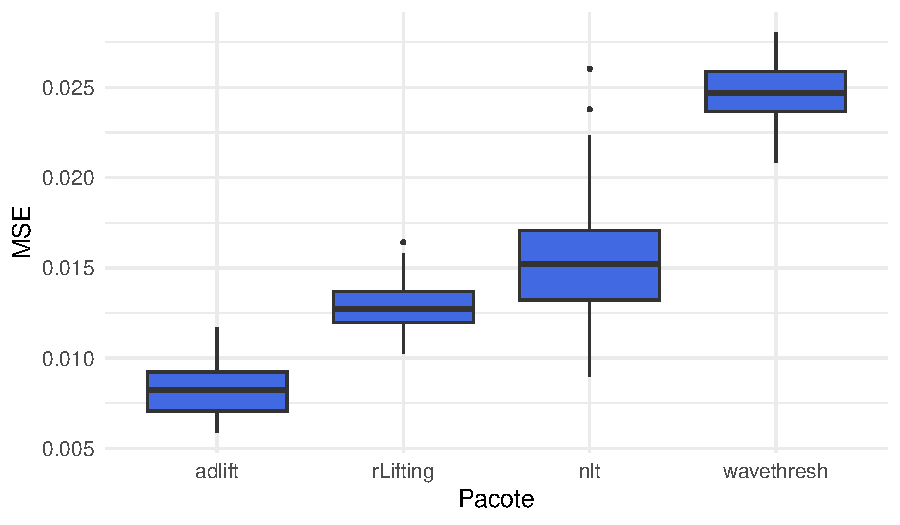
\includegraphics[width=0.75\textwidth]{figuras/benchmark_mse.pdf}
    \caption{MSE mediano na melhor configuração de cada pacote, por sinal de referência (\(T=1024\), grade regular, 1000 replicações de Monte Carlo). Menores valores indicam melhor desempenho.}
    \label{fig:rlifting-benchmark-mse}
\end{figure}

Por fim, demonstramos a capacidade de processamento em tempo real na Figura \ref{fig:realtime-denoising}. 
Nela, simulamos um fluxo contínuo de dados ruidosos (uma senoide com ruído) sendo processado ponto a ponto pelo \texttt{new\_wavelet\_stream}. 
A cada nova observação, o algoritmo atualiza a estimativa instantânea (linha azul) em tempo constante, sem acesso a dados futuros. 
O resultado evidencia que o pacote consegue recuperar a tendência subjacente do sinal (linha tracejada) com pouco atraso, viabilizando seu uso em sistemas de monitoramento \emph{online}.

\begin{figure}[H]
    \centering
    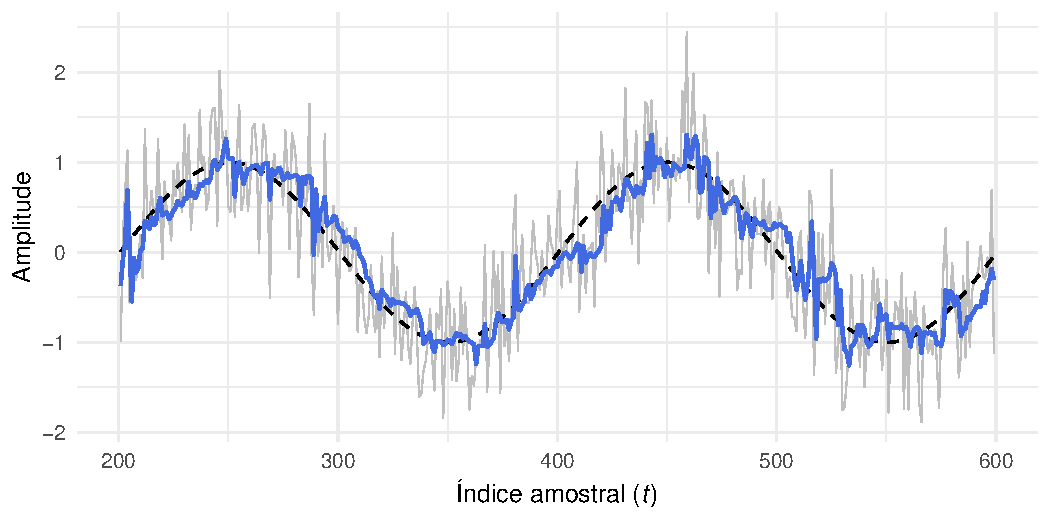
\includegraphics[width=0.75\textwidth]{figuras/realtime_denoising.pdf}
    \caption{Suavização em tempo real de um fluxo de dados. A linha sólida (azul) representa a estimativa calculada incrementalmente pelo \texttt{rLifting} à medida que novos pontos (cinza) são observados. A linha preta tracejada é a função original.}
    \label{fig:realtime-denoising}
\end{figure}

Esses resultados reforçam que o \texttt{rLifting} ocupa um nicho distinto ao oferecer a velocidade necessária para aplicações intensivas ou de tempo real, mantendo uma qualidade de reconstrução comparável às implementações já existentes da DWT.

\section{Considerações práticas de implementação}\label{sec-metodologia-consideracoes}
Nesta seção, discutimos algumas das escolhas paramétricas e limitações imediatas da nossa proposta metodológica que influenciam o desenho dos experimentos apresentados no Capítulo \ref{sec-estudos-simulacao}. 
Adiantamos que retomaremos a discussão de limitações mais fundamentais no Capítulo \ref{sec-conclusao}.

O primeiro ponto de ponderação para um analista no procedimento operacionalmente causal é a escolha do tamanho da janela móvel, \(W\). 
Janelas curtas irão reagir rapidamente a mudanças de regime no tempo real, mas limitam o nível de resolução máximo da DWT e podem inviabilizar a detecção de tendências de longo prazo. 
Uma janela excessivamente longa, todavia, faz com que a DWT \emph{online} aproxime-se de sua contraparte \emph{offline}, com a restrição, porém, de que as primeiras \(W\) observações do sinal retornado ainda estarão contaminadas pelo ruído. 
Como recomendação geral, é uma boa prática verificar informações disponíveis sobre o tamanho total do sinal, se possível, antes de determinar \(W\).

Problema similar acomete as escolhas dos hiperparâmetros \(\alpha\) e \(\beta\). 
Os valores padrão funcionam bem para uma gama de funções, mas o algoritmo pode desempenhar melhor com uma calibração mais cuidadosa. 
Para análises \emph{offline} ou em lote, a função \texttt{tune\_alpha\_beta()} seleciona \(\alpha\) e \(\beta\) minimizando o SURE sobre uma grade de parâmetros com refinamento via Nelder-Mead. 
O custo computacional é da ordem de segundos para \(T \sim 10^3\), o que a torna inviável para aplicações em tempo real estrito. 
Uma via alternativa é \texttt{threshold\_method = "sure"}, que contorna \(\alpha\) e \(\beta\) por completo, calibrando cada nível de resolução individualmente via SURE sem recorrer à recursão paramétrica. 
Em processamento por janela, o parâmetro \texttt{update\_freq} completa esse quadro ao controlar com que frequência os limiares são recalculados. 
O padrão, recálculo a cada nova amostra, maximiza a adaptabilidade, mas valores maiores reduzem o custo computacional em cenários de dados volumosos.

Ainda em relação ao \texttt{rLifting}, métodos de pré-processamento \emph{online} invariavelmente apresentam atraso de borda. 
Para procedimentos em que a causalidade operacional é necessária, recomendamos fortemente o uso de filtros mais curtos (como Haar e Daubechies 2). 
Filtros como CDF 9/7 exigem que mais pontos sejam artificialmente inseridos pela extensão de borda, o que pode comprometer a reconstrução da função subjacente. 
Este é um tópico especialmente relevante para a estimação do \(\mathrm{FATE}\), uma vez que são precisamente os pontos de borda que alimentam a regressão via mínimos quadrados nos procedimentos \emph{online}. 
O leitor há de notar que em nossas simulações fomos precavidos em relação a essa problemática.

Finalmente, conquanto seja possível construir as bandas de confiança para fluxos de estimação operacionalmente causais em cenários que não exijam a velocidade de atualizações instantâneas, gostaríamos de reiterar a impossibilidade computacional de obtenção dessas bandas para aplicações em tempo real estrito. 
Como paliativo, para estes casos mais complexos computacionalmente, sugerimos uma atualização periódica das bandas. 
Reconhecemos que essa estratégia introduz um atraso entre a obtenção dos resultados pontuais e das bandas de confiança, mas acreditamos que estes, a depender do problema, seriam toleráveis: se o fluxo de dados for alto (rápida atualização de dados), rapidamente teríamos pontos amostrais suficientes para os procedimentos de reamostragem. 
Embora a latência exista, não tardaria até que pudéssemos identificar falhas no modelo; se, por outro lado, o fluxo de dados for lento, teríamos tempo suficiente para executar o \emph{bootstrap}, efetivamente eliminando o atraso entre estimativas pontuais e intervalares.
\chapter[Estudos de simulação]{Estudos de simulação}\label{sec-estudos-simulacao}
A fim de avaliar o comportamento empírico dos estimadores propostos, conduzimos dois estudos de simulação principais. O primeiro compara a nossa proposta baseada em ondaletas --- Seção \ref{sec-estimacao-fate} em suas versões \emph{offline} e \emph{online} --- com o estimador de \emph{splines} utilizado em \citeonline{ecker_causal_2024} (Seção \ref{sec-inferencia-causal-funcional}). Como já discutido, ao adotarmos o mesmo processo gerador de dados (PGD) e o cenário de intervenção única dos autores, tornamos a exigência de causalidade operacional (respeito à seta do tempo) optativa. Esse desenho nos permite comparar diretamente a eficiência da suavização e a identificação do efeito entre os métodos, estabelecendo o estimador \emph{offline} como um teto teórico de desempenho para a versão \emph{online}.\footnote{Uma vez que o cenário não requer o respeito à causalidade operacional, o estimador \emph{offline} deve desempenhar melhor que o \emph{online} em virtude de ter acesso a uma quantidade maior de informação.} A segunda simulação, por sua vez, foca exclusivamente em nosso estimador \emph{online} (Seção \ref{sec-estimador-online}; tendo em vista que não encontramos abordagens alternativas para estimar o \(\mathrm{FATE}\) sequencialmente na literatura), mensurando a latência computacional do processamento ponto a ponto e a precisão da estimativa quando as observações de cada indivíduo são disponibilizadas sequencialmente, sem que o estimador tenha acesso a informações futuras --- por óbvio, o desempenho estatístico do estimador \emph{online} não deve mudar significativamente de um desenho experimental para outro. A única diferença entre os estimadores é que, na primeira simulação, utilizamos a função \texttt{denoise\_signal\_causal}, enquanto na segunda, emulamos os dados chegando sequencialmente com \texttt{new\_wavelet\_stream}. Ambas as funções estão disponíveis no ecossistema do \texttt{rLifting}.

Em nosso desenho, buscamos mimetizar o PGD de \citeonline{ecker_causal_2024} para garantir uma base de comparação mais sólida. Geramos \(P = 9\) covariáveis pré-tratamento amostradas de distribuições Normal, Poisson e Binomial, cujos parâmetros foram calibrados com base nas estatísticas descritivas reportadas no trabalho original (Tabela \ref{tab:parametros_pgd}). A atribuição de tratamento segue um modelo logístico com viés de seleção induzido, e as propensões foram truncadas no intervalo \([0.001, 0.999]\) para assegurar a positividade condicional. O desfecho funcional é gerado a partir de um modelo concorrente no qual o efeito de tratamento é heterogêneo, dependendo das covariáveis observadas. Distribuímos o efeito total uniformemente entre o intercepto e as \(9\) covariáveis, de modo que cada componente contribua igualmente para o \(\mathrm{FATE}\) verdadeiro através da média populacional \(\bar{\mathbf{X}}\).

A fim de exemplificar os ganhos de nossos estimadores, quando comparado ao PGD de \citeonline{ecker_causal_2024}, ampliamos o conjunto de formas funcionais avaliadas. Consideramos funções de efeito com os formatos: \emph{sigmoide}, \emph{bumps}, \emph{doppler} e \emph{escada}. Esperávamos, a priori, que o estimador original, baseado em \emph{splines}, desempenhasse mal nos últimos três cenários supracitados.

Em ambas as simulações cruzamos tamanhos de amostra \(N \in \{200, 500, 2000\}\) com resoluções temporais \(T \in \{128, 256, 512\}\). Para o pré-processamento via ondaletas, a família mãe foi selecionada conforme o cenário (utilizamos filtros curtos para o caso \emph{online}, conforme nossa discussão metodológica, e para o caso \emph{offline}, por comparabilidade; e.g., Haar para o cenário Escada e Daubechies-2 para Bumps), enquanto para os \emph{splines} utilizamos o padrão de \(50\) funções de base em todos os casos (otimizamos o procedimento via validação cruzada generalizada --- o que é de praxe e, inclusive, é feito por \citeonline{ecker_causal_2024}, apesar de teoricamente afetar a normalidade esperada do estimador \(\hat{\theta}(t)\) resultante). Onde aplicável, a janela de processamento causal foi fixada em \(W = 64\) para resoluções menores e \(W = 128\) para \(T = 512\), permitindo um equilíbrio entre a estabilidade da reconstrução e o respeito à seta do tempo. 

Obtemos as estimativas intervalares para os métodos baseados em ondaletas através do procedimento descrito na Seção \ref{sec-bootstrap-ic}. Para as \emph{splines}, utilizamos as derivações analíticas de \citeonline{ecker_causal_2024}. Vale salientar, no entanto, que introduzimos uma escolha deliberadamente conservadora na calibração do limiar de cobertura \(u_\alpha(t)\). Em vez de utilizar a estrutura variável original, baseada no pacote \texttt{ffscb} \cite{lieblFastFairSimultaneous2023}, fixamos um limiar escalar constante correspondente ao valor mais conservador do referido pacote. O objetivo desta modificação era assegurar que eventuais falhas de cobertura do método original em cenários irregulares não decorressem de bandas excessivamente estreitas localmente. Estratégia que nos permite uma avaliação mais isolada do impacto da falta de regularidade na estimativa pontual. Essa escolha, é claro, inviabiliza a comparação das larguras de banda resultantes de nosso \emph{bootstrap}, para com o método de \citeonline{ecker_causal_2024} (no fim das contas, mesmo com nossas precauções, a comparação seria inócua, tendo em vista que a metodologia original não se mostrou estatisticamente confiável para cenários irregulares mesmo com larguras de banda artificialmente maiores).

\begin{table}[ht]
	\centering
	\caption{Especificação paramétrica do processo gerador de dados das simulações.}
	\label{tab:parametros_pgd}
	\begin{tabular}{llrr}
		\toprule
		Covariável & Distribuição & Escore de propensão & Efeito concorrente \\
		\midrule
		\(X_{i1}\) & \(\mathrm{N}(-2.3;\ 1.2^2)\) & \(-0.052\) & \(-0.02\) \\
		\(X_{i2}\) & \(\mathrm{N}(8.3;\ 4.1^2)\) & \(-0.001\) & \(0.5\exp(-2t)\) \\
		\(X_{i3}\) & \(\mathrm{Bin}(1;\ 0.019)\) & \(0.020\) & \(-0.1 + 0.2(t-0.5)^2\) \\
		\(X_{i4}\) & \(\mathrm{Bin}(1;\ 0.710)\) & \(-0.097\) & \(0.2t\) \\
		\(X_{i5}\) & \(\mathrm{Pois}(2.3)\) & \(-0.056\) & \(0.01\sin(10t)\) \\
		\(X_{i6}\) & \(\mathrm{N}(11.8;\ 0.9^2)\) & \(0.510\) & \(0.05\) \\
		\(X_{i7}\) & \(\mathrm{Bin}(1;\ 0.023)\) & \(0.568\) & \(-0.1\) \\
		\(X_{i8}\) & \(\mathrm{Bin}(1;\ 0.297)\) & \(0.674\) & \(0.1\exp(-t)\) \\
		\(X_{i9}\) & \(\mathrm{Bin}(1;\ 0.112)\) & \(0.851\) & \(0.15\exp(-t)\) \\
		\bottomrule
	\end{tabular}
\end{table}

Para avaliar o desempenho dos estimadores, consideramos métricas de precisão pontual e global, além de propriedades de cobertura das bandas de confiança simultâneas. Denotamos por \(\theta(t_k)\) o efeito populacional verdadeiro no instante \(t_k \equiv k\) (com \(k = 0, \dots, T-1\)) e por \(\hat{\theta}^{(r)}(t_k)\) a sua respectiva estimativa obtida na réplica \(r = 1, \dots, R\) da simulação (com \(R = 1000\)).

Iniciamos pela avaliação da precisão em cada instante de tempo, calculando o erro quadrático médio e o viés pontuais através da média sobre as \(R\) réplicas:
\begin{equation}
	\mathrm{RMSE}(t_k) = \sqrt{\frac{1}{R}\sum_{r=1}^{R} \bigl(\hat{\theta}^{(r)}(t_k) - \theta(t_k)\bigr)^2}, \quad \text{Viés}(t_k) = \frac{1}{R}\sum_{r=1}^{R} \bigl(\hat{\theta}^{(r)}(t_k) - \theta(t_k)\bigr)
\end{equation}
Essas medidas permitem visualizar a evolução do erro e a estabilidade da estimativa ao longo das trajetórias. Em seguida, definimos as métricas globais para cada réplica \(r\), agregadas sobre os \(T\) instantes de tempo:
\begin{description}
	\item[Raíz quadrada do erro quadrático médio (RMSE)] quantifica a precisão global da trajetória estimada em cada réplica:
	\begin{equation*}
		\\mathrm{RMSE}^{(r)} = \sqrt{\frac{1}{T}\sum_{k=0}^{T-1} \bigl(\hat{\theta}^{(r)}(t_k) - \theta(t_k)\bigr)^2}.
	\end{equation*}
	\item[Raíz quadrada do erro quadrático médio normalizado (NRMSE)] escalona o \text{RMSE} pela amplitude da trajetória verdadeira, facilitando a comparação entre cenários com diferentes magnitudes de efeito:
	\begin{equation*}
		\mathrm{NRMSE}^{(r)} = \frac{\text{RMSE}^{(r)}}{\max_{t_k} \theta(t_k) - \min_{t_k} \theta(t_k)}.
	\end{equation*}
	\item[Viés global] avalia o erro sistemático médio ao longo de toda a curva:
	\begin{equation*}
		\text{Viés}^{(r)} = \frac{1}{T}\sum_{k=0}^{T-1} \bigl(\hat{\theta}^{(r)}(t_k) - \theta(t_k)\bigr).
	\end{equation*}
	\item[Latência computacional] representa o tempo médio de processamento por ponto na grade temporal (exclusivo para a Simulação 2):
	\begin{equation*}
		\text{Latência}^{(r)} = \frac{1}{T}\sum_{k=0}^{T-1} \text{Tempo}(\text{Processamento ponto } k).
	\end{equation*}
	\item[Cobertura simultânea] é uma indicadora binária que assume \(1\) se, e somente se, a banda de confiança contém a trajetória verdadeira em todos os instantes \(t_k\), simultaneamente:
	\begin{equation*}
		\mathrm{CobSim}^{(r)} = \mathbb{I}\left( \forall k : \theta(t_k) \in [\hat{\theta}_{\text{low}}^{(r)}(t_k), \hat{\theta}_{\text{up}}^{(r)}(t_k)] \right).
	\end{equation*}
	\item[Largura média da banda de confiança], monitorada a fim de avaliar o custo informacional necessário para atingir o nível de confiança nominal.
	\begin{equation*}
		\(\mathrm{Largura}^{(r)} = \frac{1}{T}\sum_{k=0}^{T-1} \bigl(\hat{\theta}_{\text{up}}^{(r)}(t_k) - \hat{\theta}_{\text{low}}^{(r)}(t_k)\bigr)\)
	\end{equation*}

\end{description}

Deve-se observar, contudo, que a métrica de latência reportada representa a média de processamento por ponto na grade, obtida em ambiente controlado com hardware comercial padrão. Embora os valores absolutos possam variar conforme a infraestrutura, a estabilidade e a ordem de grandeza observada confirmam a viabilidade operacional do método para o regime sequencial pretendido.

A seguir, apresentamos os resultados obtidos. Para fins de clareza e síntese no corpo principal deste trabalho, optamos por exibir uma seleção representativa dos cenários (Sigmoid, Doppler e Escada), contrastando os extremos de resolução temporal (\(T = 128\) e \(T = 512\)) sob diferentes tamanhos de amostra. Esta escolha permite observar os padrões de convergência e as vantagens competitivas da metodologia proposta sem sobrecarregar a leitura com a totalidade das combinações simuladas. Os resultados exaustivos para todos os cenários e resoluções encontram-se detalhados no Apêndice \ref{ap-simulacoes-completas}.

Note que, para fins de clareza visual, as distribuições de erro (\(\mathrm{NRMSE}\)) e largura de banda nas figuras subsequentes são representadas pela mediana e pelos quartis de 25\% e 75\%, de modo a omitir valores atípicos que dificultariam a percepção visual do impacto das resoluções \(T\) e \(N\).

\section{Resultados}

Abaixo, apresentamos as tabelas gerenciais que condensam o desempenho dos métodos avaliados. No que tange à Simulação 1, focamos na comparação direta entre Ondaletas e Splines de Ecker para os cenários mais desafiadores.

\begin{table}[ht]
	\centering
	\caption{Desempenho estatístico comparado (Simulação 1) --- Resultados Selecionados.}
	\label{tab:resultados_sim1}
	\scriptsize
	\begin{tabular}{llccrrrr}
		\toprule
		Cenário & Método & \(N\) & \(T\) & \(\text{RMSE}\) & \(\text{NRMSE}\) & \(\text{Vício}\) & \(\text{CobSim}\) \\
\midrule
\multirow{18}{*}{Sigmoid} & Ond. (On) & 200 & 128 & 1,278 & 0,574 & 0,055 & 85,9\% \\
 & Ond. (Off) & 200 & 128 & 1,304 & 0,585 & 0,058 & 86,6\% \\
 & Ecker & 200 & 128 & 1,300 & 0,584 & 0,058 & 100,0\% \\
\cmidrule{2-8}
 & Ond. (On) & 200 & 512 & 1,199 & 0,538 & 0,106 & 88,9\% \\
 & Ond. (Off) & 200 & 512 & 1,206 & 0,541 & 0,107 & 89,5\% \\
 & Ecker & 200 & 512 & 1,205 & 0,541 & 0,107 & 100,0\% \\
\cmidrule{2-8}
 & Ond. (On) & 500 & 128 & 0,091 & 0,041 & 0,009 & 96,8\% \\
 & Ond. (Off) & 500 & 128 & 0,099 & 0,044 & 0,011 & 97,4\% \\
 & Ecker & 500 & 128 & 0,091 & 0,041 & 0,011 & 100,0\% \\
\cmidrule{2-8}
 & Ond. (On) & 500 & 512 & 0,102 & 0,046 & 0,007 & 96,1\% \\
 & Ond. (Off) & 500 & 512 & 0,103 & 0,046 & 0,008 & 96,9\% \\
 & Ecker & 500 & 512 & 0,102 & 0,046 & 0,008 & 100,0\% \\
\cmidrule{2-8}
 & Ond. (On) & 2000 & 128 & 0,022 & 0,010 & -0,001 & 96,1\% \\
 & Ond. (Off) & 2000 & 128 & 0,034 & 0,015 & 0,001 & 94,7\% \\
 & Ecker & 2000 & 128 & 0,022 & 0,010 & 0,001 & 100,0\% \\
\cmidrule{2-8}
 & Ond. (On) & 2000 & 512 & 0,021 & 0,010 & -0,001 & 94,6\% \\
 & Ond. (Off) & 2000 & 512 & 0,023 & 0,010 & 0,000 & 95,0\% \\
 & Ecker & 2000 & 512 & 0,021 & 0,010 & 0,000 & 100,0\% \\
\cmidrule{2-8}
\midrule
\multirow{18}{*}{Doppler} & Ond. (On) & 200 & 128 & 1,785 & 0,161 & 0,027 & 86,8\% \\
 & Ond. (Off) & 200 & 128 & 1,716 & 0,155 & 0,044 & 86,8\% \\
 & Ecker & 200 & 128 & 2,806 & 0,253 & 0,051 & 40,1\% \\
\cmidrule{2-8}
 & Ond. (On) & 200 & 512 & 1,498 & 0,135 & 0,071 & 87,1\% \\
 & Ond. (Off) & 200 & 512 & 1,253 & 0,113 & 0,078 & 87,1\% \\
 & Ecker & 200 & 512 & 2,337 & 0,210 & 0,079 & 40,3\% \\
\cmidrule{2-8}
 & Ond. (On) & 500 & 128 & 0,805 & 0,073 & -0,003 & 96,1\% \\
 & Ond. (Off) & 500 & 128 & 0,722 & 0,065 & 0,014 & 95,8\% \\
 & Ecker & 500 & 128 & 2,011 & 0,182 & 0,021 & 3,8\% \\
\cmidrule{2-8}
 & Ond. (On) & 500 & 512 & 0,467 & 0,042 & -0,001 & 96,2\% \\
 & Ond. (Off) & 500 & 512 & 0,136 & 0,012 & 0,006 & 96,8\% \\
 & Ecker & 500 & 512 & 1,493 & 0,134 & 0,007 & 3,0\% \\
\cmidrule{2-8}
 & Ond. (On) & 2000 & 128 & 0,736 & 0,066 & -0,025 & 94,9\% \\
 & Ond. (Off) & 2000 & 128 & 0,650 & 0,059 & -0,008 & 94,8\% \\
 & Ecker & 2000 & 128 & 1,960 & 0,177 & -0,001 & 0,0\% \\
\cmidrule{2-8}
 & Ond. (On) & 2000 & 512 & 0,406 & 0,037 & -0,008 & 96,2\% \\
 & Ond. (Off) & 2000 & 512 & 0,060 & 0,005 & -0,001 & 95,2\% \\
 & Ecker & 2000 & 512 & 1,445 & 0,130 & 0,000 & 0,0\% \\
\cmidrule{2-8}
\midrule
\multirow{18}{*}{Escada} & Ond. (On) & 200 & 128 & 1,235 & 0,046 & 0,084 & 87,2\% \\
 & Ond. (Off) & 200 & 128 & 1,257 & 0,047 & 0,077 & 88,0\% \\
 & Ecker & 200 & 128 & 2,283 & 0,086 & 0,077 & 40,8\% \\
\cmidrule{2-8}
 & Ond. (On) & 200 & 512 & 1,347 & 0,050 & 0,088 & 85,7\% \\
 & Ond. (Off) & 200 & 512 & 1,354 & 0,051 & 0,087 & 86,0\% \\
 & Ecker & 200 & 512 & 2,100 & 0,079 & 0,087 & 42,7\% \\
\cmidrule{2-8}
 & Ond. (On) & 500 & 128 & 0,125 & 0,005 & 0,005 & 97,7\% \\
 & Ond. (Off) & 500 & 128 & 0,127 & 0,005 & -0,003 & 97,2\% \\
 & Ecker & 500 & 128 & 1,427 & 0,053 & -0,003 & 3,4\% \\
\cmidrule{2-8}
 & Ond. (On) & 500 & 512 & 0,086 & 0,003 & 0,027 & 97,4\% \\
 & Ond. (Off) & 500 & 512 & 0,086 & 0,003 & 0,026 & 97,3\% \\
 & Ecker & 500 & 512 & 1,073 & 0,040 & 0,026 & 2,6\% \\
\cmidrule{2-8}
 & Ond. (On) & 2000 & 128 & 0,049 & 0,002 & 0,008 & 95,4\% \\
 & Ond. (Off) & 2000 & 128 & 0,050 & 0,002 & 0,000 & 95,9\% \\
 & Ecker & 2000 & 128 & 1,379 & 0,052 & 0,000 & 0,0\% \\
\cmidrule{2-8}
 & Ond. (On) & 2000 & 512 & 0,022 & 0,001 & 0,001 & 95,5\% \\
 & Ond. (Off) & 2000 & 512 & 0,022 & 0,001 & 0,000 & 95,7\% \\
 & Ecker & 2000 & 512 & 1,040 & 0,039 & 0,000 & 0,0\% \\
\cmidrule{2-8}
		\bottomrule
	\end{tabular}
\end{table}

\begin{table}[ht]
	\centering
	\caption{Eficiência computacional e confiabilidade (Simulação 2) --- Ondaletas Online.}
	\label{tab:resultados_sim2}
	\begin{tabular}{lcrrrrr}
		\toprule
		Cenário & \(T\) & \(N\) & \(\text{RMSE}\) & \(\text{NRMSE}\) & \(\text{Vício}\) & \(\text{Latência (µs)}\) \\
\midrule
\multirow{9}{*}{Bumps} & 128 & 200 & 1,391 & 0,022 & 0,244 & 3,7 \\
 & 128 & 500 & 0,180 & 0,003 & 0,009 & 3,9 \\
 & 128 & 2000 & 0,116 & 0,002 & -0,015 & 4,1 \\
\cmidrule{2-7}
 & 256 & 200 & 1,323 & 0,020 & 0,041 & 4,2 \\
 & 256 & 500 & 0,208 & 0,003 & 0,028 & 4,2 \\
 & 256 & 2000 & 0,122 & 0,002 & -0,021 & 5,1 \\
\cmidrule{2-7}
 & 512 & 200 & 1,432 & 0,021 & -0,058 & 5,3 \\
 & 512 & 500 & 0,101 & 0,002 & 0,017 & 5,4 \\
 & 512 & 2000 & 0,040 & 0,001 & -0,002 & 6,9 \\
\cmidrule{2-7}
\midrule
\multirow{9}{*}{Doppler} & 128 & 200 & 1,827 & 0,165 & 0,015 & 3,7 \\
 & 128 & 500 & 0,771 & 0,070 & -0,024 & 3,8 \\
 & 128 & 2000 & 0,736 & 0,066 & -0,024 & 4,1 \\
\cmidrule{2-7}
 & 256 & 200 & 1,937 & 0,175 & 0,048 & 4,2 \\
 & 256 & 500 & 0,952 & 0,086 & -0,049 & 4,2 \\
 & 256 & 2000 & 0,852 & 0,077 & -0,067 & 7,6 \\
\cmidrule{2-7}
 & 512 & 200 & 1,586 & 0,143 & 0,101 & 5,3 \\
 & 512 & 500 & 0,480 & 0,043 & 0,001 & 5,5 \\
 & 512 & 2000 & 0,405 & 0,036 & -0,008 & 8,7 \\
\cmidrule{2-7}
\midrule
\multirow{9}{*}{Heavisine} & 128 & 200 & 1,245 & 0,047 & 0,041 & 3,5 \\
 & 128 & 500 & 0,115 & 0,004 & 0,003 & 3,6 \\
 & 128 & 2000 & 0,049 & 0,002 & 0,008 & 3,9 \\
\cmidrule{2-7}
 & 256 & 200 & 1,457 & 0,055 & 0,119 & 4,0 \\
 & 256 & 500 & 0,114 & 0,004 & 0,001 & 4,0 \\
 & 256 & 2000 & 0,031 & 0,001 & 0,004 & 4,3 \\
\cmidrule{2-7}
 & 512 & 200 & 1,106 & 0,041 & 0,061 & 4,7 \\
 & 512 & 500 & 0,081 & 0,003 & 0,026 & 5,0 \\
 & 512 & 2000 & 0,023 & 0,001 & 0,001 & 5,2 \\
\cmidrule{2-7}
\midrule
\multirow{9}{*}{Sigmoid} & 128 & 200 & 1,315 & 0,591 & 0,046 & 3,6 \\
 & 128 & 500 & 0,093 & 0,042 & 0,006 & 3,6 \\
 & 128 & 2000 & 0,022 & 0,010 & -0,001 & 3,9 \\
\cmidrule{2-7}
 & 256 & 200 & 1,179 & 0,529 & 0,135 & 4,0 \\
 & 256 & 500 & 0,085 & 0,038 & 0,008 & 4,0 \\
 & 256 & 2000 & 0,022 & 0,010 & -0,002 & 4,7 \\
\cmidrule{2-7}
 & 512 & 200 & 1,295 & 0,582 & 0,083 & 4,7 \\
 & 512 & 500 & 0,105 & 0,047 & 0,028 & 5,0 \\
 & 512 & 2000 & 0,021 & 0,009 & 0,000 & 5,2 \\
\cmidrule{2-7}
		\bottomrule
	\end{tabular}
\end{table}

\chapter[CONCLUSÃO]{Conclusão}\label{sec-conclusao}


% Escreva aqui as conclusões do trabalho.

% ----------------------------------------------------------
% ---------------------------------------------------------------------------------
% %%%%%%%%%%%%%%%%%%%%%%%%%% FIM DOS ELEMENTOS TEXTUAIS %%%%%%%%%%%%%%%%%%%%%%%%%%
% ---------------------------------------------------------------------------------
% ---------------------------------------------------------------------------------
% %%%%%%%%%%%%%%%%%%%%%%% INÍCIO DOS ELEMENTOS PÓS-TEXTUAIS %%%%%%%%%%%%%%%%%%%%%%%
% ---------------------------------------------------------------------------------
% ----------------------------------------------------------
\postextual
% ----------------------------------------------------------
% ----------------------------------------------------------
% REFERÊNCIAS
\bibliography{referencias.bib}
% ----------------------------------------------------------
% ----------------------------------------------------------
% APÊNDICES
\begin{apendicesenv}
  % Imprime uma página indicando o início dos apêndices
  \partapendices
  \chapter{Resultados Detalhados das Simulações}
\label{ap-simulacoes-completas}

Neste Apêndice, apresentamos a totalidade dos resultados obtidos na Simulação 1, cobrindo todos os cenários de sinal (Bumps, Doppler, Escada e Sigmoid), tamanhos de amostra (\(N = 200, 500, 2000\)) e resoluções temporais (\(T = 128, 256, 512\)).

\begin{table}[ht]
	\centering
	\caption{Desempenho estatístico completo (Simulação 1) --- Resultados exaustivos.}
	\label{tab:resultados_sim1_completo}
	\scriptsize
	\begin{tabular{llccrrrr}
		\toprule
		Cenário & Método & \(N\) & \(T\) & \(\text{RMSE}\) & \(\text{NRMSE}\) & \(\text{Vício}\) & \(\text{CobSim}\) \\
\midrule
\multirow{27}{*}{Bumps} & Ond. (On) & 200 & 128 & 1,334 & 0,021 & 0,131 & 86,0\% \\
 & Ond. (Off) & 200 & 128 & 1,298 & 0,021 & 0,148 & 86,1\% \\
 & Ecker & 200 & 128 & 7,007 & 0,113 & 0,147 & 40,8\% \\
\cmidrule{2-8}
 & Ond. (On) & 200 & 256 & 1,349 & 0,020 & 0,067 & 86,0\% \\
 & Ond. (Off) & 200 & 256 & 1,303 & 0,019 & 0,088 & 86,0\% \\
 & Ecker & 200 & 256 & 5,270 & 0,078 & 0,087 & 42,3\% \\
\cmidrule{2-8}
 & Ond. (On) & 200 & 512 & 1,294 & 0,019 & 0,182 & 86,5\% \\
 & Ond. (Off) & 200 & 512 & 1,290 & 0,019 & 0,183 & 86,7\% \\
 & Ecker & 200 & 512 & 5,308 & 0,079 & 0,183 & 42,7\% \\
\cmidrule{2-8}
 & Ond. (On) & 500 & 128 & 0,203 & 0,003 & -0,012 & 96,2\% \\
 & Ond. (Off) & 500 & 128 & 0,149 & 0,002 & 0,005 & 96,3\% \\
 & Ecker & 500 & 128 & 6,569 & 0,106 & 0,004 & 3,9\% \\
\cmidrule{2-8}
 & Ond. (On) & 500 & 256 & 0,199 & 0,003 & -0,040 & 96,9\% \\
 & Ond. (Off) & 500 & 256 & 0,130 & 0,002 & -0,019 & 96,3\% \\
 & Ecker & 500 & 256 & 4,728 & 0,070 & -0,019 & 3,9\% \\
\cmidrule{2-8}
 & Ond. (On) & 500 & 512 & 0,138 & 0,002 & -0,009 & 95,3\% \\
 & Ond. (Off) & 500 & 512 & 0,131 & 0,002 & -0,007 & 96,3\% \\
 & Ecker & 500 & 512 & 4,770 & 0,071 & -0,007 & 3,1\% \\
\cmidrule{2-8}
 & Ond. (On) & 2000 & 128 & 0,116 & 0,002 & -0,016 & 94,7\% \\
 & Ond. (Off) & 2000 & 128 & 0,056 & 0,001 & 0,001 & 94,8\% \\
 & Ecker & 2000 & 128 & 6,546 & 0,105 & -0,001 & 0,0\% \\
\cmidrule{2-8}
 & Ond. (On) & 2000 & 256 & 0,122 & 0,002 & -0,020 & 93,9\% \\
 & Ond. (Off) & 2000 & 256 & 0,045 & 0,001 & 0,001 & 93,7\% \\
 & Ecker & 2000 & 256 & 4,694 & 0,070 & 0,000 & 0,0\% \\
\cmidrule{2-8}
 & Ond. (On) & 2000 & 512 & 0,040 & 0,001 & -0,002 & 94,1\% \\
 & Ond. (Off) & 2000 & 512 & 0,030 & 0,000 & 0,000 & 96,0\% \\
 & Ecker & 2000 & 512 & 4,738 & 0,071 & 0,000 & 0,0\% \\
\cmidrule{2-8}
\midrule
\multirow{27}{*}{Doppler} & Ond. (On) & 200 & 128 & 1,785 & 0,161 & 0,027 & 86,8\% \\
 & Ond. (Off) & 200 & 128 & 1,716 & 0,155 & 0,044 & 86,8\% \\
 & Ecker & 200 & 128 & 2,806 & 0,253 & 0,051 & 40,1\% \\
\cmidrule{2-8}
 & Ond. (On) & 200 & 256 & 2,033 & 0,183 & -0,057 & 84,2\% \\
 & Ond. (Off) & 200 & 256 & 1,534 & 0,138 & 0,007 & 85,2\% \\
 & Ecker & 200 & 256 & 2,517 & 0,227 & 0,010 & 43,7\% \\
\cmidrule{2-8}
 & Ond. (On) & 200 & 512 & 1,498 & 0,135 & 0,071 & 87,1\% \\
 & Ond. (Off) & 200 & 512 & 1,253 & 0,113 & 0,078 & 87,1\% \\
 & Ecker & 200 & 512 & 2,337 & 0,210 & 0,079 & 40,3\% \\
\cmidrule{2-8}
 & Ond. (On) & 500 & 128 & 0,805 & 0,073 & -0,003 & 96,1\% \\
 & Ond. (Off) & 500 & 128 & 0,722 & 0,065 & 0,014 & 95,8\% \\
 & Ecker & 500 & 128 & 2,011 & 0,182 & 0,021 & 3,8\% \\
\cmidrule{2-8}
 & Ond. (On) & 500 & 256 & 0,944 & 0,085 & -0,024 & 95,8\% \\
 & Ond. (Off) & 500 & 256 & 0,290 & 0,026 & 0,041 & 96,0\% \\
 & Ecker & 500 & 256 & 1,542 & 0,139 & 0,044 & 3,9\% \\
\cmidrule{2-8}
 & Ond. (On) & 500 & 512 & 0,467 & 0,042 & -0,001 & 96,2\% \\
 & Ond. (Off) & 500 & 512 & 0,136 & 0,012 & 0,006 & 96,8\% \\
 & Ecker & 500 & 512 & 1,493 & 0,134 & 0,007 & 3,0\% \\
\cmidrule{2-8}
 & Ond. (On) & 2000 & 128 & 0,736 & 0,066 & -0,025 & 94,9\% \\
 & Ond. (Off) & 2000 & 128 & 0,650 & 0,059 & -0,008 & 94,8\% \\
 & Ecker & 2000 & 128 & 1,960 & 0,177 & -0,001 & 0,0\% \\
\cmidrule{2-8}
 & Ond. (On) & 2000 & 256 & 0,852 & 0,077 & -0,067 & 94,5\% \\
 & Ond. (Off) & 2000 & 256 & 0,181 & 0,016 & -0,003 & 95,5\% \\
 & Ecker & 2000 & 256 & 1,460 & 0,132 & 0,001 & 0,0\% \\
\cmidrule{2-8}
 & Ond. (On) & 2000 & 512 & 0,406 & 0,037 & -0,008 & 96,2\% \\
 & Ond. (Off) & 2000 & 512 & 0,060 & 0,005 & -0,001 & 95,2\% \\
 & Ecker & 2000 & 512 & 1,445 & 0,130 & 0,000 & 0,0\% \\
\cmidrule{2-8}
\midrule
\multirow{27}{*}{Escada} & Ond. (On) & 200 & 128 & 1,235 & 0,046 & 0,084 & 87,2\% \\
 & Ond. (Off) & 200 & 128 & 1,257 & 0,047 & 0,077 & 88,0\% \\
 & Ecker & 200 & 128 & 2,283 & 0,086 & 0,077 & 40,8\% \\
\cmidrule{2-8}
 & Ond. (On) & 200 & 256 & 1,234 & 0,046 & -0,022 & 88,2\% \\
 & Ond. (Off) & 200 & 256 & 1,245 & 0,047 & -0,027 & 88,5\% \\
 & Ecker & 200 & 256 & 1,982 & 0,074 & -0,027 & 41,8\% \\
\cmidrule{2-8}
 & Ond. (On) & 200 & 512 & 1,347 & 0,050 & 0,088 & 85,7\% \\
 & Ond. (Off) & 200 & 512 & 1,354 & 0,051 & 0,087 & 86,0\% \\
 & Ecker & 200 & 512 & 2,100 & 0,079 & 0,087 & 42,7\% \\
\cmidrule{2-8}
 & Ond. (On) & 500 & 128 & 0,125 & 0,005 & 0,005 & 97,7\% \\
 & Ond. (Off) & 500 & 128 & 0,127 & 0,005 & -0,003 & 97,2\% \\
 & Ecker & 500 & 128 & 1,427 & 0,053 & -0,003 & 3,4\% \\
\cmidrule{2-8}
 & Ond. (On) & 500 & 256 & 0,106 & 0,004 & -0,017 & 96,2\% \\
 & Ond. (Off) & 500 & 256 & 0,104 & 0,004 & -0,021 & 96,4\% \\
 & Ecker & 500 & 256 & 1,058 & 0,040 & -0,021 & 3,4\% \\
\cmidrule{2-8}
 & Ond. (On) & 500 & 512 & 0,086 & 0,003 & 0,027 & 97,4\% \\
 & Ond. (Off) & 500 & 512 & 0,086 & 0,003 & 0,026 & 97,3\% \\
 & Ecker & 500 & 512 & 1,073 & 0,040 & 0,026 & 2,6\% \\
\cmidrule{2-8}
 & Ond. (On) & 2000 & 128 & 0,049 & 0,002 & 0,008 & 95,4\% \\
 & Ond. (Off) & 2000 & 128 & 0,050 & 0,002 & 0,000 & 95,9\% \\
 & Ecker & 2000 & 128 & 1,379 & 0,052 & 0,000 & 0,0\% \\
\cmidrule{2-8}
 & Ond. (On) & 2000 & 256 & 0,032 & 0,001 & 0,004 & 93,5\% \\
 & Ond. (Off) & 2000 & 256 & 0,028 & 0,001 & 0,000 & 93,9\% \\
 & Ecker & 2000 & 256 & 1,014 & 0,038 & 0,000 & 0,0\% \\
\cmidrule{2-8}
 & Ond. (On) & 2000 & 512 & 0,022 & 0,001 & 0,001 & 95,5\% \\
 & Ond. (Off) & 2000 & 512 & 0,022 & 0,001 & 0,000 & 95,7\% \\
 & Ecker & 2000 & 512 & 1,040 & 0,039 & 0,000 & 0,0\% \\
\cmidrule{2-8}
\midrule
\multirow{27}{*}{Sigmoid} & Ond. (On) & 200 & 128 & 1,278 & 0,574 & 0,055 & 85,9\% \\
 & Ond. (Off) & 200 & 128 & 1,304 & 0,585 & 0,058 & 86,6\% \\
 & Ecker & 200 & 128 & 1,300 & 0,584 & 0,058 & 100,0\% \\
\cmidrule{2-8}
 & Ond. (On) & 200 & 256 & 1,353 & 0,607 & -0,001 & 86,0\% \\
 & Ond. (Off) & 200 & 256 & 1,368 & 0,614 & 0,001 & 86,6\% \\
 & Ecker & 200 & 256 & 1,367 & 0,614 & 0,001 & 100,0\% \\
\cmidrule{2-8}
 & Ond. (On) & 200 & 512 & 1,199 & 0,538 & 0,106 & 88,9\% \\
 & Ond. (Off) & 200 & 512 & 1,206 & 0,541 & 0,107 & 89,5\% \\
 & Ecker & 200 & 512 & 1,205 & 0,541 & 0,107 & 100,0\% \\
\cmidrule{2-8}
 & Ond. (On) & 500 & 128 & 0,091 & 0,041 & 0,009 & 96,8\% \\
 & Ond. (Off) & 500 & 128 & 0,099 & 0,044 & 0,011 & 97,4\% \\
 & Ecker & 500 & 128 & 0,091 & 0,041 & 0,011 & 100,0\% \\
\cmidrule{2-8}
 & Ond. (On) & 500 & 256 & 0,118 & 0,053 & 0,005 & 96,7\% \\
 & Ond. (Off) & 500 & 256 & 0,121 & 0,054 & 0,007 & 96,6\% \\
 & Ecker & 500 & 256 & 0,118 & 0,053 & 0,007 & 100,0\% \\
\cmidrule{2-8}
 & Ond. (On) & 500 & 512 & 0,102 & 0,046 & 0,007 & 96,1\% \\
 & Ond. (Off) & 500 & 512 & 0,103 & 0,046 & 0,008 & 96,9\% \\
 & Ecker & 500 & 512 & 0,102 & 0,046 & 0,008 & 100,0\% \\
\cmidrule{2-8}
 & Ond. (On) & 2000 & 128 & 0,022 & 0,010 & -0,001 & 96,1\% \\
 & Ond. (Off) & 2000 & 128 & 0,034 & 0,015 & 0,001 & 94,7\% \\
 & Ecker & 2000 & 128 & 0,022 & 0,010 & 0,001 & 100,0\% \\
\cmidrule{2-8}
 & Ond. (On) & 2000 & 256 & 0,022 & 0,010 & -0,002 & 95,2\% \\
 & Ond. (Off) & 2000 & 256 & 0,026 & 0,012 & 0,000 & 94,8\% \\
 & Ecker & 2000 & 256 & 0,021 & 0,009 & 0,000 & 100,0\% \\
\cmidrule{2-8}
 & Ond. (On) & 2000 & 512 & 0,021 & 0,010 & -0,001 & 94,6\% \\
 & Ond. (Off) & 2000 & 512 & 0,023 & 0,010 & 0,000 & 95,0\% \\
 & Ecker & 2000 & 512 & 0,021 & 0,010 & 0,000 & 100,0\% \\
\cmidrule{2-8}
		\bottomrule
	\end{tabular}
\end{table}

\end{apendicesenv}
% ----------------------------------------------------------
% ----------------------------------------------------------
% ANEXOS
% \begin{anexosenv}
%   % Imprime uma página indicando o início dos anexos
%   \partanexos
%   \include{7-anexos}
% \end{anexosenv}
% ----------------------------------------------------------
% ----------------------------------------------------------
% ---------------------------------------------------------------------------------
% %%%%%%%%%%%%%%%%%%%%%%%%%% FIM DOS ELEMENTOS TEXTUAIS %%%%%%%%%%%%%%%%%%%%%%%%%%
% ----------------------------------------------------------------------------------
% -----------------------------------------------------------------------------------------------
% %%%%%%%%%%%%%%%%%%%%%%%%%%%%%%%%%%%%%% FIM DO DOCUMENTO %%%%%%%%%%%%%%%%%%%%%%%%%%%%%%%%%%%%%%
% -----------------------------------------------------------------------------------------------
\end{document}
